
%...........................................................
%
% Predicted number of events
%
%...........................................................

\section{Effect of systematic uncertainties}
\label{app:systematics}

In \cref{tab:apply_syst_to_template_mulike_fhc},
\cref{tab:apply_syst_to_template_elike_fhc},
\cref{tab:apply_syst_to_template_mulike_rhc} and
\cref{tab:apply_syst_to_template_elike_fhc}
it is shown which systematic parameter is applied to which reaction and flavour modes 
for all the Super-K samples.
 
\afterpage{%\documentclass[10pt]{article}
%\usepackage[utf8]{inputenc}
%\usepackage{amsmath}
%\usepackage{amsfonts}
%\usepackage{amssymb}
%\usepackage{fullpage}
%\usepackage{rotate}  
%\usepackage{rotating}
%\usepackage[paperwidth=300mm,paperheight=450mm]{geometry}

%\newcommand{\ck}{$\checkmark$}
%\begin{document}

{
\setlength{\tabcolsep}{2pt}
\renewcommand{\arraystretch}{1.5}
\begin{landscape}
\begin{footnotesize}

\begin{longtable} { | c ||c | c | c | c | c | c | c | c | c | c | c | c | c | c | c | c | c | c | c | c | c | c | c | c | c | c | c | c | c | c | c | c | c | c | c | c | c | c | c | c | c | c | c | c | c | c | c | c | c | c |  | }
\hline
 & \begin{sideways} $\nu_\mu$ CCQE \end{sideways} 
 & \begin{sideways} $\nu_\mu$ CC 1$\pi$ \end{sideways} 
 & \begin{sideways} $\nu_\mu$ CC coherent \end{sideways} 
 & \begin{sideways} $\nu_\mu$ CC 2p-2h \end{sideways} 
 & \begin{sideways} $\nu_\mu$ CC other \end{sideways} 
 & \begin{sideways} $\nu_\mu$/$\nu_\tau$ NC 1$\pi^{+/-}$ \end{sideways} 
 & \begin{sideways} $\nu_\mu$/$\nu_\tau$ NC 1$\pi^0$ \end{sideways} 
 & \begin{sideways} $\nu_\mu$/$\nu_\tau$ NC coherent \end{sideways} 
 & \begin{sideways} $\nu_\mu$/$\nu_\tau$ NC other \end{sideways} 
 & \begin{sideways} $\nu_e$ NC 1$\gamma$ \end{sideways} 
 & \begin{sideways} $\bar{\nu}_\mu$ CCQE \end{sideways} 
 & \begin{sideways} $\bar{\nu}_\mu$ CC 1$\pi$ \end{sideways} 
 & \begin{sideways} $\bar{\nu}_\mu$ CC coherent \end{sideways} 
 & \begin{sideways} $\bar{\nu}_\mu$ CC 2p-2h \end{sideways} 
 & \begin{sideways} $\bar{\nu}_\mu$ CC other \end{sideways} 
 & \begin{sideways} $\bar{\nu}_\mu$/$\bar{\nu}_\tau$ NC 1$\pi^{+/-}$ \end{sideways} 
 & \begin{sideways} $\bar{\nu}_\mu$/$\bar{\nu}_\tau$ NC 1$\pi^0$ \end{sideways} 
 & \begin{sideways} $\bar{\nu}_\mu$/$\bar{\nu}_\tau$ NC coherent \end{sideways} 
 & \begin{sideways} $\bar{\nu}_\mu$/$\bar{\nu}_\tau$ NC other \end{sideways} 
 & \begin{sideways} $\nu_\mu$ NC 1$\gamma$ \end{sideways} 
 & \begin{sideways} $\nu_e$ CCQE \end{sideways} 
 & \begin{sideways} $\nu_e$ CC 1$\pi$ \end{sideways} 
 & \begin{sideways} $\nu_e$ CC coherent \end{sideways} 
 & \begin{sideways} $\nu_e$ CC 2p-2h \end{sideways} 
 & \begin{sideways} $\nu_e$ CC other \end{sideways} 
 & \begin{sideways} $\nu_e$ NC 1$\pi^{+/-}$ \end{sideways} 
 & \begin{sideways} $\nu_e$ NC 1$\pi^0$ \end{sideways} 
 & \begin{sideways} $\nu_e$ NC coherent \end{sideways} 
 & \begin{sideways} $\nu_e$ NC other \end{sideways} 
 & \begin{sideways} $\bar{\nu}_\mu$ NC 1$\gamma$ \end{sideways} 
 & \begin{sideways} Osc. $\nu_e$ CCQE \end{sideways} 
 & \begin{sideways} Osc. $\nu_e$ CC 1$\pi$ \end{sideways} 
 & \begin{sideways} Osc. $\nu_e$ CC coherent \end{sideways} 
 & \begin{sideways} Osc. $\nu_e$ CC 2p-2h \end{sideways} 
 & \begin{sideways} Osc. $\nu_e$ CC other \end{sideways} 
 & \begin{sideways} $\bar{\nu}_e$ CCQE \end{sideways} 
 & \begin{sideways} $\bar{\nu}_e$ CC 1$\pi$ \end{sideways} 
 & \begin{sideways} $\bar{\nu}_e$ CC coherent \end{sideways} 
 & \begin{sideways} $\bar{\nu}_e$ CC 2p-2h \end{sideways} 
 & \begin{sideways} $\bar{\nu}_e$ CC other \end{sideways} 
 & \begin{sideways} $\bar{\nu}_e$ NC 1$\pi^{+/-}$ \end{sideways} 
 & \begin{sideways} $\bar{\nu}_e$ NC 1$\pi^0$ \end{sideways} 
 & \begin{sideways} $\bar{\nu}_e$ NC coherent \end{sideways} 
 & \begin{sideways} $\bar{\nu}_e$ NC other \end{sideways} 
 & \begin{sideways} $\bar{\nu}_e$ NC 1$\gamma$ \end{sideways} 
 & \begin{sideways} Osc. $\bar{\nu}_e$ CCQE \end{sideways} 
 & \begin{sideways} Osc. $\bar{\nu}_e$ CC 1$\pi$ \end{sideways} 
 & \begin{sideways} Osc. $\bar{\nu}_e$ CC coherent \end{sideways} 
 & \begin{sideways} Osc. $\bar{\nu}_e$ CC 2p-2h \end{sideways} 
 & \begin{sideways} Osc. $\bar{\nu}_e$ CC other \end{sideways} 
\\ \hline 
%$\sin^2(\theta_{12})$         & \ck& \ck& \ck& \ck& \ck&    &    &    &    &    & \ck& \ck& \ck& \ck& \ck&    &    &    &    &    & \ck& \ck& \ck& \ck& \ck&    &    &    &    &    & \ck& \ck& \ck& \ck& \ck& \ck& \ck& \ck& \ck& \ck&    &    &    &    &    & \ck& \ck& \ck& \ck& \ck \\ \hline 
%$\sin^2(\theta_{13})$         & \ck& \ck& \ck& \ck& \ck&    &    &    &    &    & \ck& \ck& \ck& \ck& \ck&    &    &    &    &    & \ck& \ck& \ck& \ck& \ck&    &    &    &    &    & \ck& \ck& \ck& \ck& \ck& \ck& \ck& \ck& \ck& \ck&    &    &    &    &    & \ck& \ck& \ck& \ck& \ck \\ \hline 
%$\Delta m^2_{21}$             & \ck& \ck& \ck& \ck& \ck&    &    &    &    &    & \ck& \ck& \ck& \ck& \ck&    &    &    &    &    & \ck& \ck& \ck& \ck& \ck&    &    &    &    &    & \ck& \ck& \ck& \ck& \ck& \ck& \ck& \ck& \ck& \ck&    &    &    &    &    & \ck& \ck& \ck& \ck& \ck \\ \hline 
%$\delta_{CP}$                 & \ck& \ck& \ck& \ck& \ck&    &    &    &    &    & \ck& \ck& \ck& \ck& \ck&    &    &    &    &    & \ck& \ck& \ck& \ck& \ck&    &    &    &    &    & \ck& \ck& \ck& \ck& \ck& \ck& \ck& \ck& \ck& \ck&    &    &    &    &    & \ck& \ck& \ck& \ck& \ck \\ \hline 
$f_{E; r}^{SK}$               & \ck& \ck& \ck& \ck& \ck& \ck& \ck& \ck& \ck& \ck& \ck& \ck& \ck& \ck& \ck& \ck& \ck& \ck& \ck& \ck& \ck& \ck& \ck& \ck& \ck& \ck& \ck& \ck& \ck& \ck& \ck& \ck& \ck& \ck& \ck& \ck& \ck& \ck& \ck& \ck& \ck& \ck& \ck& \ck& \ck& \ck& \ck& \ck& \ck& \ck \\ \hline 
$f_{0; t, r}^{SK+FSI}$        & \ck&    &    & \ck&    &    &    &    &    &    & \ck&    &    & \ck&    &    &    &    &    &    &    &    &    &    &    &    &    &    &    &    &    &    &    &    &    &    &    &    &    &    &    &    &    &    &    &    &    &    &    &     \\ \hline 
$f_{1; t, r}^{SK+FSI}$        & \ck&    &    & \ck&    &    &    &    &    &    & \ck&    &    & \ck&    &    &    &    &    &    &    &    &    &    &    &    &    &    &    &    &    &    &    &    &    &    &    &    &    &    &    &    &    &    &    &    &    &    &    &     \\ \hline 
$f_{2; t, r}^{SK+FSI}$        & \ck&    &    & \ck&    &    &    &    &    &    & \ck&    &    & \ck&    &    &    &    &    &    &    &    &    &    &    &    &    &    &    &    &    &    &    &    &    &    &    &    &    &    &    &    &    &    &    &    &    &    &    &     \\ \hline 
$f_{3; t, r}^{SK+FSI}$        &    & \ck& \ck&    & \ck&    &    &    &    &    &    & \ck& \ck&    & \ck&    &    &    &    &    &    &    &    &    &    &    &    &    &    &    &    &    &    &    &    &    &    &    &    &    &    &    &    &    &    &    &    &    &    &     \\ \hline 
$f_{4; t, r}^{SK+FSI}$        &    &    &    &    &    &    &    &    &    &    &    &    &    &    &    &    &    &    &    &    & \ck& \ck& \ck& \ck& \ck&    &    &    &    &    & \ck& \ck& \ck& \ck& \ck& \ck& \ck& \ck& \ck& \ck&    &    &    &    &    & \ck& \ck& \ck& \ck& \ck \\ \hline 
$f_{5; t, r}^{SK+FSI}$        &    &    &    &    &    & \ck& \ck& \ck& \ck& \ck&    &    &    &    &    & \ck& \ck& \ck& \ck& \ck&    &    &    &    &    & \ck& \ck& \ck& \ck& \ck&    &    &    &    &    &    &    &    &    &    & \ck& \ck& \ck& \ck& \ck&    &    &    &    &     \\ \hline 
$f_{0; t, r}^{banff}$         & \ck& \ck& \ck& \ck& \ck& \ck& \ck& \ck& \ck& \ck&    &    &    &    &    &    &    &    &    &    &    &    &    &    &    &    &    &    &    &    & \ck& \ck& \ck& \ck& \ck&    &    &    &    &    &    &    &    &    &    &    &    &    &    &     \\ \hline 
$f_{1; t, r}^{banff}$         & \ck& \ck& \ck& \ck& \ck& \ck& \ck& \ck& \ck& \ck&    &    &    &    &    &    &    &    &    &    &    &    &    &    &    &    &    &    &    &    & \ck& \ck& \ck& \ck& \ck&    &    &    &    &    &    &    &    &    &    &    &    &    &    &     \\ \hline 
$f_{2; t, r}^{banff}$         & \ck& \ck& \ck& \ck& \ck& \ck& \ck& \ck& \ck& \ck&    &    &    &    &    &    &    &    &    &    &    &    &    &    &    &    &    &    &    &    & \ck& \ck& \ck& \ck& \ck&    &    &    &    &    &    &    &    &    &    &    &    &    &    &     \\ \hline 
$f_{3; t, r}^{banff}$         & \ck& \ck& \ck& \ck& \ck& \ck& \ck& \ck& \ck& \ck&    &    &    &    &    &    &    &    &    &    &    &    &    &    &    &    &    &    &    &    & \ck& \ck& \ck& \ck& \ck&    &    &    &    &    &    &    &    &    &    &    &    &    &    &     \\ \hline 
$f_{4; t, r}^{banff}$         & \ck& \ck& \ck& \ck& \ck& \ck& \ck& \ck& \ck& \ck&    &    &    &    &    &    &    &    &    &    &    &    &    &    &    &    &    &    &    &    & \ck& \ck& \ck& \ck& \ck&    &    &    &    &    &    &    &    &    &    &    &    &    &    &     \\ \hline 
$f_{5; t, r}^{banff}$         & \ck& \ck& \ck& \ck& \ck& \ck& \ck& \ck& \ck& \ck&    &    &    &    &    &    &    &    &    &    &    &    &    &    &    &    &    &    &    &    & \ck& \ck& \ck& \ck& \ck&    &    &    &    &    &    &    &    &    &    &    &    &    &    &     \\ \hline 
$f_{6; t, r}^{banff}$         & \ck& \ck& \ck& \ck& \ck& \ck& \ck& \ck& \ck& \ck&    &    &    &    &    &    &    &    &    &    &    &    &    &    &    &    &    &    &    &    & \ck& \ck& \ck& \ck& \ck&    &    &    &    &    &    &    &    &    &    &    &    &    &    &     \\ \hline 
$f_{7; t, r}^{banff}$         & \ck& \ck& \ck& \ck& \ck& \ck& \ck& \ck& \ck& \ck&    &    &    &    &    &    &    &    &    &    &    &    &    &    &    &    &    &    &    &    & \ck& \ck& \ck& \ck& \ck&    &    &    &    &    &    &    &    &    &    &    &    &    &    &     \\ \hline 
$f_{8; t, r}^{banff}$         & \ck& \ck& \ck& \ck& \ck& \ck& \ck& \ck& \ck& \ck&    &    &    &    &    &    &    &    &    &    &    &    &    &    &    &    &    &    &    &    & \ck& \ck& \ck& \ck& \ck&    &    &    &    &    &    &    &    &    &    &    &    &    &    &     \\ \hline 
$f_{9; t, r}^{banff}$         & \ck& \ck& \ck& \ck& \ck& \ck& \ck& \ck& \ck& \ck&    &    &    &    &    &    &    &    &    &    &    &    &    &    &    &    &    &    &    &    & \ck& \ck& \ck& \ck& \ck&    &    &    &    &    &    &    &    &    &    &    &    &    &    &     \\ \hline 
$f_{10; t, r}^{banff}$        & \ck& \ck& \ck& \ck& \ck& \ck& \ck& \ck& \ck& \ck&    &    &    &    &    &    &    &    &    &    &    &    &    &    &    &    &    &    &    &    & \ck& \ck& \ck& \ck& \ck&    &    &    &    &    &    &    &    &    &    &    &    &    &    &     \\ \hline 
$f_{11; t, r}^{banff}$        &    &    &    &    &    &    &    &    &    &    & \ck& \ck& \ck& \ck& \ck& \ck& \ck& \ck& \ck& \ck&    &    &    &    &    &    &    &    &    &    &    &    &    &    &    &    &    &    &    &    &    &    &    &    &    & \ck& \ck& \ck& \ck& \ck \\ \hline 
$f_{12; t, r}^{banff}$        &    &    &    &    &    &    &    &    &    &    & \ck& \ck& \ck& \ck& \ck& \ck& \ck& \ck& \ck& \ck&    &    &    &    &    &    &    &    &    &    &    &    &    &    &    &    &    &    &    &    &    &    &    &    &    & \ck& \ck& \ck& \ck& \ck \\ \hline 
$f_{13; t, r}^{banff}$        &    &    &    &    &    &    &    &    &    &    & \ck& \ck& \ck& \ck& \ck& \ck& \ck& \ck& \ck& \ck&    &    &    &    &    &    &    &    &    &    &    &    &    &    &    &    &    &    &    &    &    &    &    &    &    & \ck& \ck& \ck& \ck& \ck \\ \hline 
$f_{14; t, r}^{banff}$        &    &    &    &    &    &    &    &    &    &    & \ck& \ck& \ck& \ck& \ck& \ck& \ck& \ck& \ck& \ck&    &    &    &    &    &    &    &    &    &    &    &    &    &    &    &    &    &    &    &    &    &    &    &    &    & \ck& \ck& \ck& \ck& \ck \\ \hline 
$f_{15; t, r}^{banff}$        &    &    &    &    &    &    &    &    &    &    & \ck& \ck& \ck& \ck& \ck& \ck& \ck& \ck& \ck& \ck&    &    &    &    &    &    &    &    &    &    &    &    &    &    &    &    &    &    &    &    &    &    &    &    &    & \ck& \ck& \ck& \ck& \ck \\ \hline 
$f_{16; t, r}^{banff}$        &    &    &    &    &    &    &    &    &    &    &    &    &    &    &    &    &    &    &    &    & \ck& \ck& \ck& \ck& \ck& \ck& \ck& \ck& \ck& \ck&    &    &    &    &    &    &    &    &    &    &    &    &    &    &    &    &    &    &    &     \\ \hline 
$f_{17; t, r}^{banff}$        &    &    &    &    &    &    &    &    &    &    &    &    &    &    &    &    &    &    &    &    & \ck& \ck& \ck& \ck& \ck& \ck& \ck& \ck& \ck& \ck&    &    &    &    &    &    &    &    &    &    &    &    &    &    &    &    &    &    &    &     \\ \hline 
$f_{18; t, r}^{banff}$        &    &    &    &    &    &    &    &    &    &    &    &    &    &    &    &    &    &    &    &    & \ck& \ck& \ck& \ck& \ck& \ck& \ck& \ck& \ck& \ck&    &    &    &    &    &    &    &    &    &    &    &    &    &    &    &    &    &    &    &     \\ \hline 
$f_{19; t, r}^{banff}$        &    &    &    &    &    &    &    &    &    &    &    &    &    &    &    &    &    &    &    &    & \ck& \ck& \ck& \ck& \ck& \ck& \ck& \ck& \ck& \ck&    &    &    &    &    &    &    &    &    &    &    &    &    &    &    &    &    &    &    &     \\ \hline 
$f_{20; t, r}^{banff}$        &    &    &    &    &    &    &    &    &    &    &    &    &    &    &    &    &    &    &    &    & \ck& \ck& \ck& \ck& \ck& \ck& \ck& \ck& \ck& \ck&    &    &    &    &    &    &    &    &    &    &    &    &    &    &    &    &    &    &    &     \\ \hline 
$f_{21; t, r}^{banff}$        &    &    &    &    &    &    &    &    &    &    &    &    &    &    &    &    &    &    &    &    & \ck& \ck& \ck& \ck& \ck& \ck& \ck& \ck& \ck& \ck&    &    &    &    &    &    &    &    &    &    &    &    &    &    &    &    &    &    &    &     \\ \hline 
$f_{22; t, r}^{banff}$        &    &    &    &    &    &    &    &    &    &    &    &    &    &    &    &    &    &    &    &    & \ck& \ck& \ck& \ck& \ck& \ck& \ck& \ck& \ck& \ck&    &    &    &    &    &    &    &    &    &    &    &    &    &    &    &    &    &    &    &     \\ \hline 
$f_{23; t, r}^{banff}$        &    &    &    &    &    &    &    &    &    &    &    &    &    &    &    &    &    &    &    &    &    &    &    &    &    &    &    &    &    &    &    &    &    &    &    & \ck& \ck& \ck& \ck& \ck& \ck& \ck& \ck& \ck& \ck&    &    &    &    &     \\ \hline 
$f_{24; t, r}^{banff}$        &    &    &    &    &    &    &    &    &    &    &    &    &    &    &    &    &    &    &    &    &    &    &    &    &    &    &    &    &    &    &    &    &    &    &    & \ck& \ck& \ck& \ck& \ck& \ck& \ck& \ck& \ck& \ck&    &    &    &    &     \\ \hline 
$f_{M_A^{QE}}^{banff}$        & \ck&    &    &    &    &    &    &    &    &    & \ck&    &    &    &    &    &    &    &    &    & \ck&    &    &    &    &    &    &    &    &    & \ck&    &    &    &    & \ck&    &    &    &    &    &    &    &    &    & \ck&    &    &    &     \\ \hline 
$f_{M_A^{RES}}^{banff}$       &    & \ck&    &    &    & \ck& \ck&    &    &    &    & \ck&    &    &    & \ck& \ck&    &    &    &    & \ck&    &    &    & \ck& \ck&    &    &    &    & \ck&    &    &    &    & \ck&    &    &    & \ck& \ck&    &    &    &    & \ck&    &    &     \\ \hline 
$f_{Norm_{2p-2h}}^{banff}$      &    &    &    & \ck&    &    &    &    &    &    &    &    &    & \ck&    &    &    &    &    &    &    &    &    & \ck&    &    &    &    &    &    &    &    &    & \ck&    &    &    &    & \ck&    &    &    &    &    &    &    &    &    & \ck&     \\ \hline 
$f_{C^{A}_{5}}^{banff}$       &    & \ck&    &    &    & \ck& \ck&    &    &    &    & \ck&    &    &    & \ck& \ck&    &    &    &    & \ck&    &    &    & \ck& \ck&    &    &    &    & \ck&    &    &    &    & \ck&    &    &    & \ck& \ck&    &    &    &    & \ck&    &    &     \\ \hline 
$f_{Bg_{RES}}^{banff}$        &    & \ck&    &    &    & \ck& \ck&    &    &    &    & \ck&    &    &    & \ck& \ck&    &    &    &    & \ck&    &    &    & \ck& \ck&    &    &    &    & \ck&    &    &    &    & \ck&    &    &    & \ck& \ck&    &    &    &    & \ck&    &    &     \\ \hline 
$f_{p_{f}}^{banff}$           & \ck&    &    &    &    &    &    &    &    &    & \ck&    &    &    &    &    &    &    &    &    & \ck&    &    &    &    &    &    &    &    &    & \ck&    &    &    &    & \ck&    &    &    &    &    &    &    &    &    & \ck&    &    &    &     \\ \hline 
$f_{Shape_{CCoth}}^{banff}$   &    &    &    &    & \ck&    &    &    &    &    &    &    &    &    & \ck&    &    &    &    &    &    &    &    &    & \ck&    &    &    &    &    &    &    &    &    & \ck&    &    &    &    & \ck&    &    &    &    &    &    &    &    &    & \ck \\ \hline 
$f_{E_{B}}^{banff}$           & \ck&    &    &    &    &    &    &    &    &    & \ck&    &    &    &    &    &    &    &    &    & \ck&    &    &    &    &    &    &    &    &    & \ck&    &    &    &    & \ck&    &    &    &    &    &    &    &    &    & \ck&    &    &    &     \\ \hline 
$f_{Norm_{CCcoh}}^{banff}$    &    &    & \ck&    &    &    &    &    &    &    &    &    & \ck&    &    &    &    &    &    &    &    &    & \ck&    &    &    &    &    &    &    &    &    & \ck&    &    &    &    & \ck&    &    &    &    &    &    &    &    &    & \ck&    &     \\ \hline 
$f_{Norm_{NCcoh}}^{banff}$    &    &    &    &    &    &    &    & \ck&    &    &    &    &    &    &    &    &    & \ck&    &    &    &    &    &    &    &    &    & \ck&    &    &    &    &    &    &    &    &    &    &    &    &    &    & \ck&    &    &    &    &    &    &     \\ \hline 
$f_{Norm_{NCother}}^{banff}$  &    &    &    &    &    &    &    &    & \ck&    &    &    &    &    &    &    &    &    & \ck&    &    &    &    &    &    &    &    &    & \ck&    &    &    &    &    &    &    &    &    &    &    &    &    &    & \ck&    &    &    &    &    &     \\ \hline 
$f_{Norm_{\nu_e \rightarrow \nu_\mu}}^{banff}$&    &    &    &    &    &    &    &    &    &    &    &    &    &    &    &    &    &    &    &    & \ck& \ck& \ck& \ck& \ck&    &    &    &    &    & \ck& \ck& \ck& \ck& \ck&    &    &    &    &    &    &    &    &    &    &    &    &    &    &     \\ \hline 
$f_{Norm_{NC1\gamma}}^{banff}$&    &    &    &    &    &    &    &    &    & \ck&    &    &    &    &    &    &    &    &    & \ck&    &    &    &    &    &    &    &    &    & \ck&    &    &    &    &    &    &    &    &    &    &    &    &    &    & \ck&    &    &    &    &     \\ \hline 
$f_{Norm_{\bar{\nu}_e \rightarrow \bar{\nu}_\mu}}^{banff}$&    &    &    &    &    &    &    &    &    &    &    &    &    &    &    &    &    &    &    &    &    &    &    &    &    &    &    &    &    &    &    &    &    &    &    & \ck& \ck& \ck& \ck& \ck&    &    &    &    &    & \ck& \ck& \ck& \ck& \ck \\ \hline 
$f_{Norm_{2p-2h-Bar}}^{banff}$   &    &    &    &    &    &    &    &    &    &    &    &    &    & \ck&    &    &    &    &    &    &    &    &    &    &    &    &    &    &    &    &    &    &    &    &    &    &    &    & \ck&    &    &    &    &    &    &    &    &    & \ck&     \\ \hline 

\caption{
Each row of this table represents one of the \NSyst systematic parameters (oscillation excluded) considered in this analysis and each column represents 
 one of the \NMCTemplate{} MC templates used to construct the single $\mu$-like ring reconstructed energy spectrum p.d.f. in neutrino mode. 
 A \ck symbol denotes that the given MC template is modified when the given systematic parameter is tweaked.
 Only the systematic parameters that affect this sample are shown.
     % \huge{TO UPDATE} % caption is already ok
}
\label{tab:apply_syst_to_template_mulike_fhc}
\end{longtable}
\end{footnotesize}
\end{landscape}
}
}
\afterpage{%\documentclass[10pt]{article}
%\usepackage[utf8]{inputenc}
%\usepackage{amsmath}
%\usepackage{amsfonts}
%\usepackage{amssymb}
%\usepackage{fullpage}
%\usepackage{rotate}  
%\usepackage{rotating}
%\usepackage[paperwidth=300mm,paperheight=450mm]{geometry}

%\newcommand{\ck}{$\checkmark$}
%\begin{document}

{
\setlength{\tabcolsep}{2pt}
\renewcommand{\arraystretch}{1.5}
\begin{landscape}
\begin{footnotesize}

\begin{longtable} { | c ||c | c | c | c | c | c | c | c | c | c | c | c | c | c | c | c | c | c | c | c | c | c | c | c | c | c | c | c | c | c | c | c | c | c | c | c | c | c | c | c | c | c | c | c | c | c | c | c | c | c |  | }
\hline
 & \begin{sideways} $\nu_\mu$ CCQE \end{sideways} 
 & \begin{sideways} $\nu_\mu$ CC 1$\pi$ \end{sideways} 
 & \begin{sideways} $\nu_\mu$ CC coherent \end{sideways} 
 & \begin{sideways} $\nu_\mu$ CC 2p-2h \end{sideways} 
 & \begin{sideways} $\nu_\mu$ CC other \end{sideways} 
 & \begin{sideways} $\nu_\mu$/$\nu_\tau$ NC 1$\pi^{+/-}$ \end{sideways} 
 & \begin{sideways} $\nu_\mu$/$\nu_\tau$ NC 1$\pi^0$ \end{sideways} 
 & \begin{sideways} $\nu_\mu$/$\nu_\tau$ NC coherent \end{sideways} 
 & \begin{sideways} $\nu_\mu$/$\nu_\tau$ NC other \end{sideways} 
 & \begin{sideways} $\nu_e$ NC 1$\gamma$ \end{sideways} 
 & \begin{sideways} $\bar{\nu}_\mu$ CCQE \end{sideways} 
 & \begin{sideways} $\bar{\nu}_\mu$ CC 1$\pi$ \end{sideways} 
 & \begin{sideways} $\bar{\nu}_\mu$ CC coherent \end{sideways} 
 & \begin{sideways} $\bar{\nu}_\mu$ CC 2p-2h \end{sideways} 
 & \begin{sideways} $\bar{\nu}_\mu$ CC other \end{sideways} 
 & \begin{sideways} $\bar{\nu}_\mu$/$\bar{\nu}_\tau$ NC 1$\pi^{+/-}$ \end{sideways} 
 & \begin{sideways} $\bar{\nu}_\mu$/$\bar{\nu}_\tau$ NC 1$\pi^0$ \end{sideways} 
 & \begin{sideways} $\bar{\nu}_\mu$/$\bar{\nu}_\tau$ NC coherent \end{sideways} 
 & \begin{sideways} $\bar{\nu}_\mu$/$\bar{\nu}_\tau$ NC other \end{sideways} 
 & \begin{sideways} $\nu_\mu$ NC 1$\gamma$ \end{sideways} 
 & \begin{sideways} $\nu_e$ CCQE \end{sideways} 
 & \begin{sideways} $\nu_e$ CC 1$\pi$ \end{sideways} 
 & \begin{sideways} $\nu_e$ CC coherent \end{sideways} 
 & \begin{sideways} $\nu_e$ CC 2p-2h \end{sideways} 
 & \begin{sideways} $\nu_e$ CC other \end{sideways} 
 & \begin{sideways} $\nu_e$ NC 1$\pi^{+/-}$ \end{sideways} 
 & \begin{sideways} $\nu_e$ NC 1$\pi^0$ \end{sideways} 
 & \begin{sideways} $\nu_e$ NC coherent \end{sideways} 
 & \begin{sideways} $\nu_e$ NC other \end{sideways} 
 & \begin{sideways} $\bar{\nu}_\mu$ NC 1$\gamma$ \end{sideways} 
 & \begin{sideways} Osc. $\nu_e$ CCQE \end{sideways} 
 & \begin{sideways} Osc. $\nu_e$ CC 1$\pi$ \end{sideways} 
 & \begin{sideways} Osc. $\nu_e$ CC coherent \end{sideways} 
 & \begin{sideways} Osc. $\nu_e$ CC 2p-2h \end{sideways} 
 & \begin{sideways} Osc. $\nu_e$ CC other \end{sideways} 
 & \begin{sideways} $\bar{\nu}_e$ CCQE \end{sideways} 
 & \begin{sideways} $\bar{\nu}_e$ CC 1$\pi$ \end{sideways} 
 & \begin{sideways} $\bar{\nu}_e$ CC coherent \end{sideways} 
 & \begin{sideways} $\bar{\nu}_e$ CC 2p-2h \end{sideways} 
 & \begin{sideways} $\bar{\nu}_e$ CC other \end{sideways} 
 & \begin{sideways} $\bar{\nu}_e$ NC 1$\pi^{+/-}$ \end{sideways} 
 & \begin{sideways} $\bar{\nu}_e$ NC 1$\pi^0$ \end{sideways} 
 & \begin{sideways} $\bar{\nu}_e$ NC coherent \end{sideways} 
 & \begin{sideways} $\bar{\nu}_e$ NC other \end{sideways} 
 & \begin{sideways} $\bar{\nu}_e$ NC 1$\gamma$ \end{sideways} 
 & \begin{sideways} Osc. $\bar{\nu}_e$ CCQE \end{sideways} 
 & \begin{sideways} Osc. $\bar{\nu}_e$ CC 1$\pi$ \end{sideways} 
 & \begin{sideways} Osc. $\bar{\nu}_e$ CC coherent \end{sideways} 
 & \begin{sideways} Osc. $\bar{\nu}_e$ CC 2p-2h \end{sideways} 
 & \begin{sideways} Osc. $\bar{\nu}_e$ CC other \end{sideways} 
\\ \hline 
%$\sin^2(\theta_{12})$         & \ck& \ck& \ck& \ck& \ck&    &    &    &    &    & \ck& \ck& \ck& \ck& \ck&    &    &    &    &    & \ck& \ck& \ck& \ck& \ck&    &    &    &    &    & \ck& \ck& \ck& \ck& \ck& \ck& \ck& \ck& \ck& \ck&    &    &    &    &    & \ck& \ck& \ck& \ck& \ck \\ \hline 
%$\sin^2(\theta_{13})$         & \ck& \ck& \ck& \ck& \ck&    &    &    &    &    & \ck& \ck& \ck& \ck& \ck&    &    &    &    &    & \ck& \ck& \ck& \ck& \ck&    &    &    &    &    & \ck& \ck& \ck& \ck& \ck& \ck& \ck& \ck& \ck& \ck&    &    &    &    &    & \ck& \ck& \ck& \ck& \ck \\ \hline 
%$\Delta m^2_{21}$             & \ck& \ck& \ck& \ck& \ck&    &    &    &    &    & \ck& \ck& \ck& \ck& \ck&    &    &    &    &    & \ck& \ck& \ck& \ck& \ck&    &    &    &    &    & \ck& \ck& \ck& \ck& \ck& \ck& \ck& \ck& \ck& \ck&    &    &    &    &    & \ck& \ck& \ck& \ck& \ck \\ \hline 
%$\delta_{CP}$                 & \ck& \ck& \ck& \ck& \ck&    &    &    &    &    & \ck& \ck& \ck& \ck& \ck&    &    &    &    &    & \ck& \ck& \ck& \ck& \ck&    &    &    &    &    & \ck& \ck& \ck& \ck& \ck& \ck& \ck& \ck& \ck& \ck&    &    &    &    &    & \ck& \ck& \ck& \ck& \ck \\ \hline 
$f_{E; r}^{SK}$               & \ck& \ck& \ck& \ck& \ck& \ck& \ck& \ck& \ck& \ck& \ck& \ck& \ck& \ck& \ck& \ck& \ck& \ck& \ck& \ck& \ck& \ck& \ck& \ck& \ck& \ck& \ck& \ck& \ck& \ck& \ck& \ck& \ck& \ck& \ck& \ck& \ck& \ck& \ck& \ck& \ck& \ck& \ck& \ck& \ck& \ck& \ck& \ck& \ck& \ck \\ \hline 
$f_{6; t, r}^{SK+FSI}$        &    &    &    &    &    &    &    &    &    &    &    &    &    &    &    &    &    &    &    &    &    &    &    &    &    &    &    &    &    &    & \ck& \ck& \ck& \ck& \ck&    &    &    &    &    &    &    &    &    &    & \ck& \ck& \ck& \ck& \ck \\ \hline 
$f_{7; t, r}^{SK+FSI}$        &    &    &    &    &    &    &    &    &    &    &    &    &    &    &    &    &    &    &    &    &    &    &    &    &    &    &    &    &    &    & \ck& \ck& \ck& \ck& \ck&    &    &    &    &    &    &    &    &    &    & \ck& \ck& \ck& \ck& \ck \\ \hline 
$f_{8; t, r}^{SK+FSI}$        &    &    &    &    &    &    &    &    &    &    &    &    &    &    &    &    &    &    &    &    &    &    &    &    &    &    &    &    &    &    & \ck& \ck& \ck& \ck& \ck&    &    &    &    &    &    &    &    &    &    & \ck& \ck& \ck& \ck& \ck \\ \hline 
$f_{9; t, r}^{SK+FSI}$        & \ck& \ck& \ck& \ck& \ck&    &    &    &    &    & \ck& \ck& \ck& \ck& \ck&    &    &    &    &    &    &    &    &    &    &    &    &    &    &    &    &    &    &    &    &    &    &    &    &    &    &    &    &    &    &    &    &    &    &     \\ \hline 
$f_{10; t, r}^{SK+FSI}$       & \ck& \ck& \ck& \ck& \ck&    &    &    &    &    & \ck& \ck& \ck& \ck& \ck&    &    &    &    &    &    &    &    &    &    &    &    &    &    &    &    &    &    &    &    &    &    &    &    &    &    &    &    &    &    &    &    &    &    &     \\ \hline 
$f_{11; t, r}^{SK+FSI}$       & \ck& \ck& \ck& \ck& \ck&    &    &    &    &    & \ck& \ck& \ck& \ck& \ck&    &    &    &    &    &    &    &    &    &    &    &    &    &    &    &    &    &    &    &    &    &    &    &    &    &    &    &    &    &    &    &    &    &    &     \\ \hline 
$f_{12; t, r}^{SK+FSI}$       &    &    &    &    &    &    &    &    &    &    &    &    &    &    &    &    &    &    &    &    & \ck& \ck& \ck& \ck& \ck&    &    &    &    &    &    &    &    &    &    & \ck& \ck& \ck& \ck& \ck&    &    &    &    &    &    &    &    &    &     \\ \hline 
$f_{13; t, r}^{SK+FSI}$       &    &    &    &    &    &    &    &    &    &    &    &    &    &    &    &    &    &    &    &    & \ck& \ck& \ck& \ck& \ck&    &    &    &    &    &    &    &    &    &    & \ck& \ck& \ck& \ck& \ck&    &    &    &    &    &    &    &    &    &     \\ \hline 
$f_{14; t, r}^{SK+FSI}$       &    &    &    &    &    &    &    &    &    &    &    &    &    &    &    &    &    &    &    &    & \ck& \ck& \ck& \ck& \ck&    &    &    &    &    &    &    &    &    &    & \ck& \ck& \ck& \ck& \ck&    &    &    &    &    &    &    &    &    &     \\ \hline 
$f_{15; t, r}^{SK+FSI}$       &    &    &    &    &    & \ck& \ck& \ck& \ck& \ck&    &    &    &    &    & \ck& \ck& \ck& \ck& \ck&    &    &    &    &    & \ck& \ck& \ck& \ck& \ck&    &    &    &    &    &    &    &    &    &    & \ck& \ck& \ck& \ck& \ck&    &    &    &    &     \\ \hline 
$f_{16; t, r}^{SK+FSI}$       &    &    &    &    &    & \ck& \ck& \ck& \ck& \ck&    &    &    &    &    & \ck& \ck& \ck& \ck& \ck&    &    &    &    &    & \ck& \ck& \ck& \ck& \ck&    &    &    &    &    &    &    &    &    &    & \ck& \ck& \ck& \ck& \ck&    &    &    &    &     \\ \hline 
$f_{17; t, r}^{SK+FSI}$       &    &    &    &    &    & \ck& \ck& \ck& \ck& \ck&    &    &    &    &    & \ck& \ck& \ck& \ck& \ck&    &    &    &    &    & \ck& \ck& \ck& \ck& \ck&    &    &    &    &    &    &    &    &    &    & \ck& \ck& \ck& \ck& \ck&    &    &    &    &     \\ \hline 
$f_{0; t, r}^{banff}$         & \ck& \ck& \ck& \ck& \ck& \ck& \ck& \ck& \ck& \ck&    &    &    &    &    &    &    &    &    &    &    &    &    &    &    &    &    &    &    &    & \ck& \ck& \ck& \ck& \ck&    &    &    &    &    &    &    &    &    &    &    &    &    &    &     \\ \hline 
$f_{1; t, r}^{banff}$         & \ck& \ck& \ck& \ck& \ck& \ck& \ck& \ck& \ck& \ck&    &    &    &    &    &    &    &    &    &    &    &    &    &    &    &    &    &    &    &    & \ck& \ck& \ck& \ck& \ck&    &    &    &    &    &    &    &    &    &    &    &    &    &    &     \\ \hline 
$f_{2; t, r}^{banff}$         & \ck& \ck& \ck& \ck& \ck& \ck& \ck& \ck& \ck& \ck&    &    &    &    &    &    &    &    &    &    &    &    &    &    &    &    &    &    &    &    & \ck& \ck& \ck& \ck& \ck&    &    &    &    &    &    &    &    &    &    &    &    &    &    &     \\ \hline 
$f_{3; t, r}^{banff}$         & \ck& \ck& \ck& \ck& \ck& \ck& \ck& \ck& \ck& \ck&    &    &    &    &    &    &    &    &    &    &    &    &    &    &    &    &    &    &    &    & \ck& \ck& \ck& \ck& \ck&    &    &    &    &    &    &    &    &    &    &    &    &    &    &     \\ \hline 
$f_{4; t, r}^{banff}$         & \ck& \ck& \ck& \ck& \ck& \ck& \ck& \ck& \ck& \ck&    &    &    &    &    &    &    &    &    &    &    &    &    &    &    &    &    &    &    &    & \ck& \ck& \ck& \ck& \ck&    &    &    &    &    &    &    &    &    &    &    &    &    &    &     \\ \hline 
$f_{5; t, r}^{banff}$         & \ck& \ck& \ck& \ck& \ck& \ck& \ck& \ck& \ck& \ck&    &    &    &    &    &    &    &    &    &    &    &    &    &    &    &    &    &    &    &    & \ck& \ck& \ck& \ck& \ck&    &    &    &    &    &    &    &    &    &    &    &    &    &    &     \\ \hline 
$f_{6; t, r}^{banff}$         & \ck& \ck& \ck& \ck& \ck& \ck& \ck& \ck& \ck& \ck&    &    &    &    &    &    &    &    &    &    &    &    &    &    &    &    &    &    &    &    & \ck& \ck& \ck& \ck& \ck&    &    &    &    &    &    &    &    &    &    &    &    &    &    &     \\ \hline 
$f_{7; t, r}^{banff}$         & \ck& \ck& \ck& \ck& \ck& \ck& \ck& \ck& \ck& \ck&    &    &    &    &    &    &    &    &    &    &    &    &    &    &    &    &    &    &    &    & \ck& \ck& \ck& \ck& \ck&    &    &    &    &    &    &    &    &    &    &    &    &    &    &     \\ \hline 
$f_{8; t, r}^{banff}$         & \ck& \ck& \ck& \ck& \ck& \ck& \ck& \ck& \ck& \ck&    &    &    &    &    &    &    &    &    &    &    &    &    &    &    &    &    &    &    &    & \ck& \ck& \ck& \ck& \ck&    &    &    &    &    &    &    &    &    &    &    &    &    &    &     \\ \hline 
$f_{9; t, r}^{banff}$         & \ck& \ck& \ck& \ck& \ck& \ck& \ck& \ck& \ck& \ck&    &    &    &    &    &    &    &    &    &    &    &    &    &    &    &    &    &    &    &    & \ck& \ck& \ck& \ck& \ck&    &    &    &    &    &    &    &    &    &    &    &    &    &    &     \\ \hline 
$f_{10; t, r}^{banff}$        & \ck& \ck& \ck& \ck& \ck& \ck& \ck& \ck& \ck& \ck&    &    &    &    &    &    &    &    &    &    &    &    &    &    &    &    &    &    &    &    & \ck& \ck& \ck& \ck& \ck&    &    &    &    &    &    &    &    &    &    &    &    &    &    &     \\ \hline 
$f_{11; t, r}^{banff}$        &    &    &    &    &    &    &    &    &    &    & \ck& \ck& \ck& \ck& \ck& \ck& \ck& \ck& \ck& \ck&    &    &    &    &    &    &    &    &    &    &    &    &    &    &    &    &    &    &    &    &    &    &    &    &    & \ck& \ck& \ck& \ck& \ck \\ \hline 
$f_{12; t, r}^{banff}$        &    &    &    &    &    &    &    &    &    &    & \ck& \ck& \ck& \ck& \ck& \ck& \ck& \ck& \ck& \ck&    &    &    &    &    &    &    &    &    &    &    &    &    &    &    &    &    &    &    &    &    &    &    &    &    & \ck& \ck& \ck& \ck& \ck \\ \hline 
$f_{13; t, r}^{banff}$        &    &    &    &    &    &    &    &    &    &    & \ck& \ck& \ck& \ck& \ck& \ck& \ck& \ck& \ck& \ck&    &    &    &    &    &    &    &    &    &    &    &    &    &    &    &    &    &    &    &    &    &    &    &    &    & \ck& \ck& \ck& \ck& \ck \\ \hline 
$f_{14; t, r}^{banff}$        &    &    &    &    &    &    &    &    &    &    & \ck& \ck& \ck& \ck& \ck& \ck& \ck& \ck& \ck& \ck&    &    &    &    &    &    &    &    &    &    &    &    &    &    &    &    &    &    &    &    &    &    &    &    &    & \ck& \ck& \ck& \ck& \ck \\ \hline 
$f_{15; t, r}^{banff}$        &    &    &    &    &    &    &    &    &    &    & \ck& \ck& \ck& \ck& \ck& \ck& \ck& \ck& \ck& \ck&    &    &    &    &    &    &    &    &    &    &    &    &    &    &    &    &    &    &    &    &    &    &    &    &    & \ck& \ck& \ck& \ck& \ck \\ \hline 
$f_{16; t, r}^{banff}$        &    &    &    &    &    &    &    &    &    &    &    &    &    &    &    &    &    &    &    &    & \ck& \ck& \ck& \ck& \ck& \ck& \ck& \ck& \ck& \ck&    &    &    &    &    &    &    &    &    &    &    &    &    &    &    &    &    &    &    &     \\ \hline 
$f_{17; t, r}^{banff}$        &    &    &    &    &    &    &    &    &    &    &    &    &    &    &    &    &    &    &    &    & \ck& \ck& \ck& \ck& \ck& \ck& \ck& \ck& \ck& \ck&    &    &    &    &    &    &    &    &    &    &    &    &    &    &    &    &    &    &    &     \\ \hline 
$f_{18; t, r}^{banff}$        &    &    &    &    &    &    &    &    &    &    &    &    &    &    &    &    &    &    &    &    & \ck& \ck& \ck& \ck& \ck& \ck& \ck& \ck& \ck& \ck&    &    &    &    &    &    &    &    &    &    &    &    &    &    &    &    &    &    &    &     \\ \hline 
$f_{19; t, r}^{banff}$        &    &    &    &    &    &    &    &    &    &    &    &    &    &    &    &    &    &    &    &    & \ck& \ck& \ck& \ck& \ck& \ck& \ck& \ck& \ck& \ck&    &    &    &    &    &    &    &    &    &    &    &    &    &    &    &    &    &    &    &     \\ \hline 
$f_{20; t, r}^{banff}$        &    &    &    &    &    &    &    &    &    &    &    &    &    &    &    &    &    &    &    &    & \ck& \ck& \ck& \ck& \ck& \ck& \ck& \ck& \ck& \ck&    &    &    &    &    &    &    &    &    &    &    &    &    &    &    &    &    &    &    &     \\ \hline 
$f_{21; t, r}^{banff}$        &    &    &    &    &    &    &    &    &    &    &    &    &    &    &    &    &    &    &    &    & \ck& \ck& \ck& \ck& \ck& \ck& \ck& \ck& \ck& \ck&    &    &    &    &    &    &    &    &    &    &    &    &    &    &    &    &    &    &    &     \\ \hline 
$f_{22; t, r}^{banff}$        &    &    &    &    &    &    &    &    &    &    &    &    &    &    &    &    &    &    &    &    & \ck& \ck& \ck& \ck& \ck& \ck& \ck& \ck& \ck& \ck&    &    &    &    &    &    &    &    &    &    &    &    &    &    &    &    &    &    &    &     \\ \hline 
$f_{23; t, r}^{banff}$        &    &    &    &    &    &    &    &    &    &    &    &    &    &    &    &    &    &    &    &    &    &    &    &    &    &    &    &    &    &    &    &    &    &    &    & \ck& \ck& \ck& \ck& \ck& \ck& \ck& \ck& \ck& \ck&    &    &    &    &     \\ \hline 
$f_{24; t, r}^{banff}$        &    &    &    &    &    &    &    &    &    &    &    &    &    &    &    &    &    &    &    &    &    &    &    &    &    &    &    &    &    &    &    &    &    &    &    & \ck& \ck& \ck& \ck& \ck& \ck& \ck& \ck& \ck& \ck&    &    &    &    &     \\ \hline 
$f_{M_A^{QE}}^{banff}$        & \ck&    &    &    &    &    &    &    &    &    & \ck&    &    &    &    &    &    &    &    &    & \ck&    &    &    &    &    &    &    &    &    & \ck&    &    &    &    & \ck&    &    &    &    &    &    &    &    &    & \ck&    &    &    &     \\ \hline 
$f_{M_A^{RES}}^{banff}$       &    & \ck&    &    &    & \ck& \ck&    &    &    &    & \ck&    &    &    & \ck& \ck&    &    &    &    & \ck&    &    &    & \ck& \ck&    &    &    &    & \ck&    &    &    &    & \ck&    &    &    & \ck& \ck&    &    &    &    & \ck&    &    &     \\ \hline 
$f_{Norm_{2p-2h}}^{banff}$      &    &    &    & \ck&    &    &    &    &    &    &    &    &    & \ck&    &    &    &    &    &    &    &    &    & \ck&    &    &    &    &    &    &    &    &    & \ck&    &    &    &    & \ck&    &    &    &    &    &    &    &    &    & \ck&     \\ \hline 
$f_{C^{A}_{5}}^{banff}$       &    & \ck&    &    &    & \ck& \ck&    &    &    &    & \ck&    &    &    & \ck& \ck&    &    &    &    & \ck&    &    &    & \ck& \ck&    &    &    &    & \ck&    &    &    &    & \ck&    &    &    & \ck& \ck&    &    &    &    & \ck&    &    &     \\ \hline 
$f_{Bg_{RES}}^{banff}$        &    & \ck&    &    &    & \ck& \ck&    &    &    &    & \ck&    &    &    & \ck& \ck&    &    &    &    & \ck&    &    &    & \ck& \ck&    &    &    &    & \ck&    &    &    &    & \ck&    &    &    & \ck& \ck&    &    &    &    & \ck&    &    &     \\ \hline 
$f_{p_{f}}^{banff}$           & \ck&    &    &    &    &    &    &    &    &    & \ck&    &    &    &    &    &    &    &    &    & \ck&    &    &    &    &    &    &    &    &    & \ck&    &    &    &    & \ck&    &    &    &    &    &    &    &    &    & \ck&    &    &    &     \\ \hline 
$f_{Shape_{CCoth}}^{banff}$   &    &    &    &    & \ck&    &    &    &    &    &    &    &    &    & \ck&    &    &    &    &    &    &    &    &    & \ck&    &    &    &    &    &    &    &    &    & \ck&    &    &    &    & \ck&    &    &    &    &    &    &    &    &    & \ck \\ \hline 
$f_{E_{B}}^{banff}$           & \ck&    &    &    &    &    &    &    &    &    & \ck&    &    &    &    &    &    &    &    &    & \ck&    &    &    &    &    &    &    &    &    & \ck&    &    &    &    & \ck&    &    &    &    &    &    &    &    &    & \ck&    &    &    &     \\ \hline 
$f_{Norm_{CCcoh}}^{banff}$    &    &    & \ck&    &    &    &    &    &    &    &    &    & \ck&    &    &    &    &    &    &    &    &    & \ck&    &    &    &    &    &    &    &    &    & \ck&    &    &    &    & \ck&    &    &    &    &    &    &    &    &    & \ck&    &     \\ \hline 
$f_{Norm_{NCcoh}}^{banff}$    &    &    &    &    &    &    &    & \ck&    &    &    &    &    &    &    &    &    & \ck&    &    &    &    &    &    &    &    &    & \ck&    &    &    &    &    &    &    &    &    &    &    &    &    &    & \ck&    &    &    &    &    &    &     \\ \hline 
$f_{Norm_{NCother}}^{banff}$  &    &    &    &    &    &    &    &    & \ck&    &    &    &    &    &    &    &    &    & \ck&    &    &    &    &    &    &    &    &    & \ck&    &    &    &    &    &    &    &    &    &    &    &    &    &    & \ck&    &    &    &    &    &     \\ \hline 
$f_{Norm_{\nu_e \rightarrow \nu_\mu}}^{banff}$&    &    &    &    &    &    &    &    &    &    &    &    &    &    &    &    &    &    &    &    & \ck& \ck& \ck& \ck& \ck&    &    &    &    &    & \ck& \ck& \ck& \ck& \ck&    &    &    &    &    &    &    &    &    &    &    &    &    &    &     \\ \hline 
$f_{Norm_{NC1\gamma}}^{banff}$&    &    &    &    &    &    &    &    &    & \ck&    &    &    &    &    &    &    &    &    & \ck&    &    &    &    &    &    &    &    &    & \ck&    &    &    &    &    &    &    &    &    &    &    &    &    &    & \ck&    &    &    &    &     \\ \hline 
$f_{Norm_{\bar{\nu}_e \rightarrow \bar{\nu}_\mu}}^{banff}$&    &    &    &    &    &    &    &    &    &    &    &    &    &    &    &    &    &    &    &    &    &    &    &    &    &    &    &    &    &    &    &    &    &    &    & \ck& \ck& \ck& \ck& \ck&    &    &    &    &    & \ck& \ck& \ck& \ck& \ck \\ \hline 
$f_{Norm_{2p-2h-Bar}}^{banff}$   &    &    &    &    &    &    &    &    &    &    &    &    &    & \ck&    &    &    &    &    &    &    &    &    &    &    &    &    &    &    &    &    &    &    &    &    &    &    &    & \ck&    &    &    &    &    &    &    &    &    & \ck&     \\ \hline 

\caption{
Each row of this table represents one of the \NSyst systematic parameters (oscillation excluded) considered in this analysis and each column represents 
 one of the \NMCTemplate{} MC templates used to construct the single $e$-like ring reconstructed energy spectrum p.d.f. in neutrino mode. 
 A \ck symbol denotes that the given MC template is modified when the given systematic parameter is tweaked.
 Only the systematic parameters that affect this sample are shown.
     % \huge{TO UPDATE} % caption is already ok
}
\label{tab:apply_syst_to_template_elike_fhc}
\end{longtable}
\end{footnotesize}
\end{landscape}
}
}
\afterpage{%\documentclass[10pt]{article}
%\usepackage[utf8]{inputenc}
%\usepackage{amsmath}
%\usepackage{amsfonts}
%\usepackage{amssymb}
%\usepackage{fullpage}
%\usepackage{rotate}  
%\usepackage{rotating}
%\usepackage[paperwidth=300mm,paperheight=450mm]{geometry}

%\newcommand{\ck}{$\checkmark$}
%\begin{document}

{
\setlength{\tabcolsep}{2pt}
\renewcommand{\arraystretch}{1.5}
\begin{landscape}
\begin{footnotesize}

\begin{longtable} { | c ||c | c | c | c | c | c | c | c | c | c | c | c | c | c | c | c | c | c | c | c | c | c | c | c | c | c | c | c | c | c | c | c | c | c | c | c | c | c | c | c | c | c | c | c | c | c | c | c | c | c |  | }
\hline
 & \begin{sideways} $\nu_\mu$ CCQE \end{sideways} 
 & \begin{sideways} $\nu_\mu$ CC 1$\pi$ \end{sideways} 
 & \begin{sideways} $\nu_\mu$ CC coherent \end{sideways} 
 & \begin{sideways} $\nu_\mu$ CC 2p-2h \end{sideways} 
 & \begin{sideways} $\nu_\mu$ CC other \end{sideways} 
 & \begin{sideways} $\nu_\mu$/$\nu_\tau$ NC 1$\pi^{+/-}$ \end{sideways} 
 & \begin{sideways} $\nu_\mu$/$\nu_\tau$ NC 1$\pi^0$ \end{sideways} 
 & \begin{sideways} $\nu_\mu$/$\nu_\tau$ NC coherent \end{sideways} 
 & \begin{sideways} $\nu_\mu$/$\nu_\tau$ NC other \end{sideways} 
 & \begin{sideways} $\nu_e$ NC 1$\gamma$ \end{sideways} 
 & \begin{sideways} $\bar{\nu}_\mu$ CCQE \end{sideways} 
 & \begin{sideways} $\bar{\nu}_\mu$ CC 1$\pi$ \end{sideways} 
 & \begin{sideways} $\bar{\nu}_\mu$ CC coherent \end{sideways} 
 & \begin{sideways} $\bar{\nu}_\mu$ CC 2p-2h \end{sideways} 
 & \begin{sideways} $\bar{\nu}_\mu$ CC other \end{sideways} 
 & \begin{sideways} $\bar{\nu}_\mu$/$\bar{\nu}_\tau$ NC 1$\pi^{+/-}$ \end{sideways} 
 & \begin{sideways} $\bar{\nu}_\mu$/$\bar{\nu}_\tau$ NC 1$\pi^0$ \end{sideways} 
 & \begin{sideways} $\bar{\nu}_\mu$/$\bar{\nu}_\tau$ NC coherent \end{sideways} 
 & \begin{sideways} $\bar{\nu}_\mu$/$\bar{\nu}_\tau$ NC other \end{sideways} 
 & \begin{sideways} $\nu_\mu$ NC 1$\gamma$ \end{sideways} 
 & \begin{sideways} $\nu_e$ CCQE \end{sideways} 
 & \begin{sideways} $\nu_e$ CC 1$\pi$ \end{sideways} 
 & \begin{sideways} $\nu_e$ CC coherent \end{sideways} 
 & \begin{sideways} $\nu_e$ CC 2p-2h \end{sideways} 
 & \begin{sideways} $\nu_e$ CC other \end{sideways} 
 & \begin{sideways} $\nu_e$ NC 1$\pi^{+/-}$ \end{sideways} 
 & \begin{sideways} $\nu_e$ NC 1$\pi^0$ \end{sideways} 
 & \begin{sideways} $\nu_e$ NC coherent \end{sideways} 
 & \begin{sideways} $\nu_e$ NC other \end{sideways} 
 & \begin{sideways} $\bar{\nu}_\mu$ NC 1$\gamma$ \end{sideways} 
 & \begin{sideways} Osc. $\nu_e$ CCQE \end{sideways} 
 & \begin{sideways} Osc. $\nu_e$ CC 1$\pi$ \end{sideways} 
 & \begin{sideways} Osc. $\nu_e$ CC coherent \end{sideways} 
 & \begin{sideways} Osc. $\nu_e$ CC 2p-2h \end{sideways} 
 & \begin{sideways} Osc. $\nu_e$ CC other \end{sideways} 
 & \begin{sideways} $\bar{\nu}_e$ CCQE \end{sideways} 
 & \begin{sideways} $\bar{\nu}_e$ CC 1$\pi$ \end{sideways} 
 & \begin{sideways} $\bar{\nu}_e$ CC coherent \end{sideways} 
 & \begin{sideways} $\bar{\nu}_e$ CC 2p-2h \end{sideways} 
 & \begin{sideways} $\bar{\nu}_e$ CC other \end{sideways} 
 & \begin{sideways} $\bar{\nu}_e$ NC 1$\pi^{+/-}$ \end{sideways} 
 & \begin{sideways} $\bar{\nu}_e$ NC 1$\pi^0$ \end{sideways} 
 & \begin{sideways} $\bar{\nu}_e$ NC coherent \end{sideways} 
 & \begin{sideways} $\bar{\nu}_e$ NC other \end{sideways} 
 & \begin{sideways} $\bar{\nu}_e$ NC 1$\gamma$ \end{sideways} 
 & \begin{sideways} Osc. $\bar{\nu}_e$ CCQE \end{sideways} 
 & \begin{sideways} Osc. $\bar{\nu}_e$ CC 1$\pi$ \end{sideways} 
 & \begin{sideways} Osc. $\bar{\nu}_e$ CC coherent \end{sideways} 
 & \begin{sideways} Osc. $\bar{\nu}_e$ CC 2p-2h \end{sideways} 
 & \begin{sideways} Osc. $\bar{\nu}_e$ CC other \end{sideways} 
\\ \hline 
%$\sin^2(\theta_{12})$         & \ck& \ck& \ck& \ck& \ck&    &    &    &    &    & \ck& \ck& \ck& \ck& \ck&    &    &    &    &    & \ck& \ck& \ck& \ck& \ck&    &    &    &    &    & \ck& \ck& \ck& \ck& \ck& \ck& \ck& \ck& \ck& \ck&    &    &    &    &    & \ck& \ck& \ck& \ck& \ck \\ \hline 
%$\sin^2(\theta_{13})$         & \ck& \ck& \ck& \ck& \ck&    &    &    &    &    & \ck& \ck& \ck& \ck& \ck&    &    &    &    &    & \ck& \ck& \ck& \ck& \ck&    &    &    &    &    & \ck& \ck& \ck& \ck& \ck& \ck& \ck& \ck& \ck& \ck&    &    &    &    &    & \ck& \ck& \ck& \ck& \ck \\ \hline 
%$\Delta m^2_{21}$             & \ck& \ck& \ck& \ck& \ck&    &    &    &    &    & \ck& \ck& \ck& \ck& \ck&    &    &    &    &    & \ck& \ck& \ck& \ck& \ck&    &    &    &    &    & \ck& \ck& \ck& \ck& \ck& \ck& \ck& \ck& \ck& \ck&    &    &    &    &    & \ck& \ck& \ck& \ck& \ck \\ \hline 
%$\delta_{CP}$                 & \ck& \ck& \ck& \ck& \ck&    &    &    &    &    & \ck& \ck& \ck& \ck& \ck&    &    &    &    &    & \ck& \ck& \ck& \ck& \ck&    &    &    &    &    & \ck& \ck& \ck& \ck& \ck& \ck& \ck& \ck& \ck& \ck&    &    &    &    &    & \ck& \ck& \ck& \ck& \ck \\ \hline 
$f_{E; r}^{SK}$               & \ck& \ck& \ck& \ck& \ck& \ck& \ck& \ck& \ck& \ck& \ck& \ck& \ck& \ck& \ck& \ck& \ck& \ck& \ck& \ck& \ck& \ck& \ck& \ck& \ck& \ck& \ck& \ck& \ck& \ck& \ck& \ck& \ck& \ck& \ck& \ck& \ck& \ck& \ck& \ck& \ck& \ck& \ck& \ck& \ck& \ck& \ck& \ck& \ck& \ck \\ \hline 
$f_{0; t, r}^{SK+FSI}RHC$     & \ck&    &    & \ck&    &    &    &    &    &    & \ck&    &    & \ck&    &    &    &    &    &    &    &    &    &    &    &    &    &    &    &    &    &    &    &    &    &    &    &    &    &    &    &    &    &    &    &    &    &    &    &     \\ \hline 
$f_{1; t, r}^{SK+FSI}RHC$     & \ck&    &    & \ck&    &    &    &    &    &    & \ck&    &    & \ck&    &    &    &    &    &    &    &    &    &    &    &    &    &    &    &    &    &    &    &    &    &    &    &    &    &    &    &    &    &    &    &    &    &    &    &     \\ \hline 
$f_{2; t, r}^{SK+FSI}RHC$     & \ck&    &    & \ck&    &    &    &    &    &    & \ck&    &    & \ck&    &    &    &    &    &    &    &    &    &    &    &    &    &    &    &    &    &    &    &    &    &    &    &    &    &    &    &    &    &    &    &    &    &    &    &     \\ \hline 
$f_{3; t, r}^{SK+FSI}RHC$     &    & \ck& \ck&    & \ck&    &    &    &    &    &    & \ck& \ck&    & \ck&    &    &    &    &    &    &    &    &    &    &    &    &    &    &    &    &    &    &    &    &    &    &    &    &    &    &    &    &    &    &    &    &    &    &     \\ \hline 
$f_{4; t, r}^{SK+FSI}RHC$     &    &    &    &    &    &    &    &    &    &    &    &    &    &    &    &    &    &    &    &    & \ck& \ck& \ck& \ck& \ck&    &    &    &    &    & \ck& \ck& \ck& \ck& \ck& \ck& \ck& \ck& \ck& \ck&    &    &    &    &    & \ck& \ck& \ck& \ck& \ck \\ \hline 
$f_{5; t, r}^{SK+FSI}RHC$     &    &    &    &    &    & \ck& \ck& \ck& \ck& \ck&    &    &    &    &    & \ck& \ck& \ck& \ck& \ck&    &    &    &    &    & \ck& \ck& \ck& \ck& \ck&    &    &    &    &    &    &    &    &    &    & \ck& \ck& \ck& \ck& \ck&    &    &    &    &     \\ \hline 
$f_{0; t, r}^{banff} RHC$     & \ck& \ck& \ck& \ck& \ck& \ck& \ck& \ck& \ck& \ck&    &    &    &    &    &    &    &    &    &    &    &    &    &    &    &    &    &    &    &    & \ck& \ck& \ck& \ck& \ck&    &    &    &    &    &    &    &    &    &    &    &    &    &    &     \\ \hline 
$f_{1; t, r}^{banff} RHC$     & \ck& \ck& \ck& \ck& \ck& \ck& \ck& \ck& \ck& \ck&    &    &    &    &    &    &    &    &    &    &    &    &    &    &    &    &    &    &    &    & \ck& \ck& \ck& \ck& \ck&    &    &    &    &    &    &    &    &    &    &    &    &    &    &     \\ \hline 
$f_{2; t, r}^{banff} RHC$     & \ck& \ck& \ck& \ck& \ck& \ck& \ck& \ck& \ck& \ck&    &    &    &    &    &    &    &    &    &    &    &    &    &    &    &    &    &    &    &    & \ck& \ck& \ck& \ck& \ck&    &    &    &    &    &    &    &    &    &    &    &    &    &    &     \\ \hline 
$f_{3; t, r}^{banff} RHC$     & \ck& \ck& \ck& \ck& \ck& \ck& \ck& \ck& \ck& \ck&    &    &    &    &    &    &    &    &    &    &    &    &    &    &    &    &    &    &    &    & \ck& \ck& \ck& \ck& \ck&    &    &    &    &    &    &    &    &    &    &    &    &    &    &     \\ \hline 
$f_{4; t, r}^{banff} RHC$     & \ck& \ck& \ck& \ck& \ck& \ck& \ck& \ck& \ck& \ck&    &    &    &    &    &    &    &    &    &    &    &    &    &    &    &    &    &    &    &    & \ck& \ck& \ck& \ck& \ck&    &    &    &    &    &    &    &    &    &    &    &    &    &    &     \\ \hline 
$f_{5; t, r}^{banff} RHC$     & \ck& \ck& \ck& \ck& \ck& \ck& \ck& \ck& \ck& \ck&    &    &    &    &    &    &    &    &    &    &    &    &    &    &    &    &    &    &    &    & \ck& \ck& \ck& \ck& \ck&    &    &    &    &    &    &    &    &    &    &    &    &    &    &     \\ \hline 
$f_{6; t, r}^{banff} RHC$     & \ck& \ck& \ck& \ck& \ck& \ck& \ck& \ck& \ck& \ck&    &    &    &    &    &    &    &    &    &    &    &    &    &    &    &    &    &    &    &    & \ck& \ck& \ck& \ck& \ck&    &    &    &    &    &    &    &    &    &    &    &    &    &    &     \\ \hline 
$f_{7; t, r}^{banff} RHC$     & \ck& \ck& \ck& \ck& \ck& \ck& \ck& \ck& \ck& \ck&    &    &    &    &    &    &    &    &    &    &    &    &    &    &    &    &    &    &    &    & \ck& \ck& \ck& \ck& \ck&    &    &    &    &    &    &    &    &    &    &    &    &    &    &     \\ \hline 
$f_{8; t, r}^{banff} RHC$     & \ck& \ck& \ck& \ck& \ck& \ck& \ck& \ck& \ck& \ck&    &    &    &    &    &    &    &    &    &    &    &    &    &    &    &    &    &    &    &    & \ck& \ck& \ck& \ck& \ck&    &    &    &    &    &    &    &    &    &    &    &    &    &    &     \\ \hline 
$f_{9; t, r}^{banff} RHC$     & \ck& \ck& \ck& \ck& \ck& \ck& \ck& \ck& \ck& \ck&    &    &    &    &    &    &    &    &    &    &    &    &    &    &    &    &    &    &    &    & \ck& \ck& \ck& \ck& \ck&    &    &    &    &    &    &    &    &    &    &    &    &    &    &     \\ \hline 
$f_{10; t, r}^{banff} RHC$    & \ck& \ck& \ck& \ck& \ck& \ck& \ck& \ck& \ck& \ck&    &    &    &    &    &    &    &    &    &    &    &    &    &    &    &    &    &    &    &    & \ck& \ck& \ck& \ck& \ck&    &    &    &    &    &    &    &    &    &    &    &    &    &    &     \\ \hline 
$f_{11; t, r}^{banff} RHC$    &    &    &    &    &    &    &    &    &    &    & \ck& \ck& \ck& \ck& \ck& \ck& \ck& \ck& \ck& \ck&    &    &    &    &    &    &    &    &    &    &    &    &    &    &    &    &    &    &    &    &    &    &    &    &    & \ck& \ck& \ck& \ck& \ck \\ \hline 
$f_{12; t, r}^{banff} RHC$    &    &    &    &    &    &    &    &    &    &    & \ck& \ck& \ck& \ck& \ck& \ck& \ck& \ck& \ck& \ck&    &    &    &    &    &    &    &    &    &    &    &    &    &    &    &    &    &    &    &    &    &    &    &    &    & \ck& \ck& \ck& \ck& \ck \\ \hline 
$f_{13; t, r}^{banff} RHC$    &    &    &    &    &    &    &    &    &    &    & \ck& \ck& \ck& \ck& \ck& \ck& \ck& \ck& \ck& \ck&    &    &    &    &    &    &    &    &    &    &    &    &    &    &    &    &    &    &    &    &    &    &    &    &    & \ck& \ck& \ck& \ck& \ck \\ \hline 
$f_{14; t, r}^{banff} RHC$    &    &    &    &    &    &    &    &    &    &    & \ck& \ck& \ck& \ck& \ck& \ck& \ck& \ck& \ck& \ck&    &    &    &    &    &    &    &    &    &    &    &    &    &    &    &    &    &    &    &    &    &    &    &    &    & \ck& \ck& \ck& \ck& \ck \\ \hline 
$f_{15; t, r}^{banff} RHC$    &    &    &    &    &    &    &    &    &    &    & \ck& \ck& \ck& \ck& \ck& \ck& \ck& \ck& \ck& \ck&    &    &    &    &    &    &    &    &    &    &    &    &    &    &    &    &    &    &    &    &    &    &    &    &    & \ck& \ck& \ck& \ck& \ck \\ \hline 
$f_{16; t, r}^{banff} RHC$    &    &    &    &    &    &    &    &    &    &    &    &    &    &    &    &    &    &    &    &    & \ck& \ck& \ck& \ck& \ck& \ck& \ck& \ck& \ck& \ck&    &    &    &    &    &    &    &    &    &    &    &    &    &    &    &    &    &    &    &     \\ \hline 
$f_{17; t, r}^{banff} RHC$    &    &    &    &    &    &    &    &    &    &    &    &    &    &    &    &    &    &    &    &    & \ck& \ck& \ck& \ck& \ck& \ck& \ck& \ck& \ck& \ck&    &    &    &    &    &    &    &    &    &    &    &    &    &    &    &    &    &    &    &     \\ \hline 
$f_{18; t, r}^{banff} RHC$    &    &    &    &    &    &    &    &    &    &    &    &    &    &    &    &    &    &    &    &    & \ck& \ck& \ck& \ck& \ck& \ck& \ck& \ck& \ck& \ck&    &    &    &    &    &    &    &    &    &    &    &    &    &    &    &    &    &    &    &     \\ \hline 
$f_{19; t, r}^{banff} RHC$    &    &    &    &    &    &    &    &    &    &    &    &    &    &    &    &    &    &    &    &    & \ck& \ck& \ck& \ck& \ck& \ck& \ck& \ck& \ck& \ck&    &    &    &    &    &    &    &    &    &    &    &    &    &    &    &    &    &    &    &     \\ \hline 
$f_{20; t, r}^{banff} RHC$    &    &    &    &    &    &    &    &    &    &    &    &    &    &    &    &    &    &    &    &    & \ck& \ck& \ck& \ck& \ck& \ck& \ck& \ck& \ck& \ck&    &    &    &    &    &    &    &    &    &    &    &    &    &    &    &    &    &    &    &     \\ \hline 
$f_{21; t, r}^{banff} RHC$    &    &    &    &    &    &    &    &    &    &    &    &    &    &    &    &    &    &    &    &    & \ck& \ck& \ck& \ck& \ck& \ck& \ck& \ck& \ck& \ck&    &    &    &    &    &    &    &    &    &    &    &    &    &    &    &    &    &    &    &     \\ \hline 
$f_{22; t, r}^{banff} RHC$    &    &    &    &    &    &    &    &    &    &    &    &    &    &    &    &    &    &    &    &    & \ck& \ck& \ck& \ck& \ck& \ck& \ck& \ck& \ck& \ck&    &    &    &    &    &    &    &    &    &    &    &    &    &    &    &    &    &    &    &     \\ \hline 
$f_{23; t, r}^{banff} RHC$    &    &    &    &    &    &    &    &    &    &    &    &    &    &    &    &    &    &    &    &    &    &    &    &    &    &    &    &    &    &    &    &    &    &    &    & \ck& \ck& \ck& \ck& \ck& \ck& \ck& \ck& \ck& \ck&    &    &    &    &     \\ \hline 
$f_{24; t, r}^{banff} RHC$    &    &    &    &    &    &    &    &    &    &    &    &    &    &    &    &    &    &    &    &    &    &    &    &    &    &    &    &    &    &    &    &    &    &    &    & \ck& \ck& \ck& \ck& \ck& \ck& \ck& \ck& \ck& \ck&    &    &    &    &     \\ \hline 
$f_{M_A^{QE}}^{banff} RHC$    & \ck&    &    &    &    &    &    &    &    &    & \ck&    &    &    &    &    &    &    &    &    & \ck&    &    &    &    &    &    &    &    &    & \ck&    &    &    &    & \ck&    &    &    &    &    &    &    &    &    & \ck&    &    &    &     \\ \hline 
$f_{M_A^{RES}}^{banff} RHC$   &    & \ck&    &    &    & \ck& \ck&    &    &    &    & \ck&    &    &    & \ck& \ck&    &    &    &    & \ck&    &    &    & \ck& \ck&    &    &    &    & \ck&    &    &    &    & \ck&    &    &    & \ck& \ck&    &    &    &    & \ck&    &    &     \\ \hline 
$f_{Norm_{2p-2h}}^{banff} RHC$  &    &    &    & \ck&    &    &    &    &    &    &    &    &    & \ck&    &    &    &    &    &    &    &    &    & \ck&    &    &    &    &    &    &    &    &    & \ck&    &    &    &    & \ck&    &    &    &    &    &    &    &    &    & \ck&     \\ \hline 
$f_{C^{A}_{5}}^{banff} RHC$   &    & \ck&    &    &    & \ck& \ck&    &    &    &    & \ck&    &    &    & \ck& \ck&    &    &    &    & \ck&    &    &    & \ck& \ck&    &    &    &    & \ck&    &    &    &    & \ck&    &    &    & \ck& \ck&    &    &    &    & \ck&    &    &     \\ \hline 
$f_{Bg_{RES}}^{banff} RHC$    &    & \ck&    &    &    & \ck& \ck&    &    &    &    & \ck&    &    &    & \ck& \ck&    &    &    &    & \ck&    &    &    & \ck& \ck&    &    &    &    & \ck&    &    &    &    & \ck&    &    &    & \ck& \ck&    &    &    &    & \ck&    &    &     \\ \hline 
$f_{p_{f}}^{banff} RHC$       & \ck&    &    &    &    &    &    &    &    &    & \ck&    &    &    &    &    &    &    &    &    & \ck&    &    &    &    &    &    &    &    &    & \ck&    &    &    &    & \ck&    &    &    &    &    &    &    &    &    & \ck&    &    &    &     \\ \hline 
$f_{Shape_{CCoth}}^{banff} RHC$&    &    &    &    & \ck&    &    &    &    &    &    &    &    &    & \ck&    &    &    &    &    &    &    &    &    & \ck&    &    &    &    &    &    &    &    &    & \ck&    &    &    &    & \ck&    &    &    &    &    &    &    &    &    & \ck \\ \hline 
$f_{E_{B}}^{banff} RHC$       & \ck&    &    &    &    &    &    &    &    &    & \ck&    &    &    &    &    &    &    &    &    & \ck&    &    &    &    &    &    &    &    &    & \ck&    &    &    &    & \ck&    &    &    &    &    &    &    &    &    & \ck&    &    &    &     \\ \hline 
$f_{Norm_{CCcoh}}^{banff} RHC$&    &    & \ck&    &    &    &    &    &    &    &    &    & \ck&    &    &    &    &    &    &    &    &    & \ck&    &    &    &    &    &    &    &    &    & \ck&    &    &    &    & \ck&    &    &    &    &    &    &    &    &    & \ck&    &     \\ \hline 
$f_{Norm_{NCcoh}}^{banff} RHC$&    &    &    &    &    &    &    & \ck&    &    &    &    &    &    &    &    &    & \ck&    &    &    &    &    &    &    &    &    & \ck&    &    &    &    &    &    &    &    &    &    &    &    &    &    & \ck&    &    &    &    &    &    &     \\ \hline 
$f_{Norm_{NCother}}^{banff} RHC$&    &    &    &    &    &    &    &    & \ck&    &    &    &    &    &    &    &    &    & \ck&    &    &    &    &    &    &    &    &    & \ck&    &    &    &    &    &    &    &    &    &    &    &    &    &    & \ck&    &    &    &    &    &     \\ \hline 
$f_{Norm_{\nu_e \rightarrow \nu_\mu}}^{banff} RHC$&    &    &    &    &    &    &    &    &    &    &    &    &    &    &    &    &    &    &    &    & \ck& \ck& \ck& \ck& \ck&    &    &    &    &    & \ck& \ck& \ck& \ck& \ck&    &    &    &    &    &    &    &    &    &    &    &    &    &    &     \\ \hline 
$f_{Norm_{NC1\gamma}}^{banff} RHC$&    &    &    &    &    &    &    &    &    & \ck&    &    &    &    &    &    &    &    &    & \ck&    &    &    &    &    &    &    &    &    & \ck&    &    &    &    &    &    &    &    &    &    &    &    &    &    & \ck&    &    &    &    &     \\ \hline 
$f_{Norm_{\bar{\nu}_e \rightarrow \bar{\nu}_\mu}}^{banff} RHC$&    &    &    &    &    &    &    &    &    &    &    &    &    &    &    &    &    &    &    &    &    &    &    &    &    &    &    &    &    &    &    &    &    &    &    & \ck& \ck& \ck& \ck& \ck&    &    &    &    &    & \ck& \ck& \ck& \ck& \ck \\ \hline 
$f_{Norm_{2p-2h-Bar}}^{banff} RHC$&    &    &    &    &    &    &    &    &    &    &    &    &    & \ck&    &    &    &    &    &    &    &    &    &    &    &    &    &    &    &    &    &    &    &    &    &    &    &    & \ck&    &    &    &    &    &    &    &    &    & \ck&     \\ \hline 

\caption{
Each row of this table represents one of the \NSyst systematic parameters (oscillation excluded) considered in this analysis and each column represents 
 one of the \NMCTemplate{} MC templates used to construct the single $\mu$-like ring reconstructed energy spectrum p.d.f. in antineutrino mode. 
 A \ck symbol denotes that the given MC template is modified when the given systematic parameter is tweaked.
 Only the systematic parameters that affect this sample are shown.
}
\label{tab:apply_syst_to_template_mulike_rhc}
\end{longtable}
\end{footnotesize}
\end{landscape}
}
}
\afterpage{%\documentclass[10pt]{article}
%\usepackage[utf8]{inputenc}
%\usepackage{amsmath}
%\usepackage{amsfonts}
%\usepackage{amssymb}
%\usepackage{fullpage}
%\usepackage{rotate}  
%\usepackage{rotating}
%\usepackage[paperwidth=300mm,paperheight=450mm]{geometry}

%\newcommand{\ck}{$\checkmark$}
%\begin{document}

{
\setlength{\tabcolsep}{2pt}
\renewcommand{\arraystretch}{1.5}
\begin{landscape}
\begin{footnotesize}

\begin{longtable} { | c ||c | c | c | c | c | c | c | c | c | c | c | c | c | c | c | c | c | c | c | c | c | c | c | c | c | c | c | c | c | c | c | c | c | c | c | c | c | c | c | c | c | c | c | c | c | c | c | c | c | c |  | }
\hline
 & \begin{sideways} $\nu_\mu$ CCQE \end{sideways} 
 & \begin{sideways} $\nu_\mu$ CC 1$\pi$ \end{sideways} 
 & \begin{sideways} $\nu_\mu$ CC coherent \end{sideways} 
 & \begin{sideways} $\nu_\mu$ CC 2p-2h \end{sideways} 
 & \begin{sideways} $\nu_\mu$ CC other \end{sideways} 
 & \begin{sideways} $\nu_\mu$/$\nu_\tau$ NC 1$\pi^{+/-}$ \end{sideways} 
 & \begin{sideways} $\nu_\mu$/$\nu_\tau$ NC 1$\pi^0$ \end{sideways} 
 & \begin{sideways} $\nu_\mu$/$\nu_\tau$ NC coherent \end{sideways} 
 & \begin{sideways} $\nu_\mu$/$\nu_\tau$ NC other \end{sideways} 
 & \begin{sideways} $\nu_e$ NC 1$\gamma$ \end{sideways} 
 & \begin{sideways} $\bar{\nu}_\mu$ CCQE \end{sideways} 
 & \begin{sideways} $\bar{\nu}_\mu$ CC 1$\pi$ \end{sideways} 
 & \begin{sideways} $\bar{\nu}_\mu$ CC coherent \end{sideways} 
 & \begin{sideways} $\bar{\nu}_\mu$ CC 2p-2h \end{sideways} 
 & \begin{sideways} $\bar{\nu}_\mu$ CC other \end{sideways} 
 & \begin{sideways} $\bar{\nu}_\mu$/$\bar{\nu}_\tau$ NC 1$\pi^{+/-}$ \end{sideways} 
 & \begin{sideways} $\bar{\nu}_\mu$/$\bar{\nu}_\tau$ NC 1$\pi^0$ \end{sideways} 
 & \begin{sideways} $\bar{\nu}_\mu$/$\bar{\nu}_\tau$ NC coherent \end{sideways} 
 & \begin{sideways} $\bar{\nu}_\mu$/$\bar{\nu}_\tau$ NC other \end{sideways} 
 & \begin{sideways} $\nu_\mu$ NC 1$\gamma$ \end{sideways} 
 & \begin{sideways} $\nu_e$ CCQE \end{sideways} 
 & \begin{sideways} $\nu_e$ CC 1$\pi$ \end{sideways} 
 & \begin{sideways} $\nu_e$ CC coherent \end{sideways} 
 & \begin{sideways} $\nu_e$ CC 2p-2h \end{sideways} 
 & \begin{sideways} $\nu_e$ CC other \end{sideways} 
 & \begin{sideways} $\nu_e$ NC 1$\pi^{+/-}$ \end{sideways} 
 & \begin{sideways} $\nu_e$ NC 1$\pi^0$ \end{sideways} 
 & \begin{sideways} $\nu_e$ NC coherent \end{sideways} 
 & \begin{sideways} $\nu_e$ NC other \end{sideways} 
 & \begin{sideways} $\bar{\nu}_\mu$ NC 1$\gamma$ \end{sideways} 
 & \begin{sideways} Osc. $\nu_e$ CCQE \end{sideways} 
 & \begin{sideways} Osc. $\nu_e$ CC 1$\pi$ \end{sideways} 
 & \begin{sideways} Osc. $\nu_e$ CC coherent \end{sideways} 
 & \begin{sideways} Osc. $\nu_e$ CC 2p-2h \end{sideways} 
 & \begin{sideways} Osc. $\nu_e$ CC other \end{sideways} 
 & \begin{sideways} $\bar{\nu}_e$ CCQE \end{sideways} 
 & \begin{sideways} $\bar{\nu}_e$ CC 1$\pi$ \end{sideways} 
 & \begin{sideways} $\bar{\nu}_e$ CC coherent \end{sideways} 
 & \begin{sideways} $\bar{\nu}_e$ CC 2p-2h \end{sideways} 
 & \begin{sideways} $\bar{\nu}_e$ CC other \end{sideways} 
 & \begin{sideways} $\bar{\nu}_e$ NC 1$\pi^{+/-}$ \end{sideways} 
 & \begin{sideways} $\bar{\nu}_e$ NC 1$\pi^0$ \end{sideways} 
 & \begin{sideways} $\bar{\nu}_e$ NC coherent \end{sideways} 
 & \begin{sideways} $\bar{\nu}_e$ NC other \end{sideways} 
 & \begin{sideways} $\bar{\nu}_e$ NC 1$\gamma$ \end{sideways} 
 & \begin{sideways} Osc. $\bar{\nu}_e$ CCQE \end{sideways} 
 & \begin{sideways} Osc. $\bar{\nu}_e$ CC 1$\pi$ \end{sideways} 
 & \begin{sideways} Osc. $\bar{\nu}_e$ CC coherent \end{sideways} 
 & \begin{sideways} Osc. $\bar{\nu}_e$ CC 2p-2h \end{sideways} 
 & \begin{sideways} Osc. $\bar{\nu}_e$ CC other \end{sideways} 
\\ \hline 
\endfirsthead
\multicolumn{47}{c}
{\tablename\ \thetable\ -- \textit{Continued from previous page}} \\
\endhead
\multicolumn{47}{r}{\textit{Continued on next page}} 
\endfoot
\endlastfoot
%$\sin^2(\theta_{12})$         & \ck& \ck& \ck& \ck& \ck&    &    &    &    &    & \ck& \ck& \ck& \ck& \ck&    &    &    &    &    & \ck& \ck& \ck& \ck& \ck&    &    &    &    &    & \ck& \ck& \ck& \ck& \ck& \ck& \ck& \ck& \ck& \ck&    &    &    &    &    & \ck& \ck& \ck& \ck& \ck \\ \hline 
%$\sin^2(\theta_{13})$         & \ck& \ck& \ck& \ck& \ck&    &    &    &    &    & \ck& \ck& \ck& \ck& \ck&    &    &    &    &    & \ck& \ck& \ck& \ck& \ck&    &    &    &    &    & \ck& \ck& \ck& \ck& \ck& \ck& \ck& \ck& \ck& \ck&    &    &    &    &    & \ck& \ck& \ck& \ck& \ck \\ \hline 
%$\Delta m^2_{21}$             & \ck& \ck& \ck& \ck& \ck&    &    &    &    &    & \ck& \ck& \ck& \ck& \ck&    &    &    &    &    & \ck& \ck& \ck& \ck& \ck&    &    &    &    &    & \ck& \ck& \ck& \ck& \ck& \ck& \ck& \ck& \ck& \ck&    &    &    &    &    & \ck& \ck& \ck& \ck& \ck \\ \hline 
%$\delta_{CP}$                 & \ck& \ck& \ck& \ck& \ck&    &    &    &    &    & \ck& \ck& \ck& \ck& \ck&    &    &    &    &    & \ck& \ck& \ck& \ck& \ck&    &    &    &    &    & \ck& \ck& \ck& \ck& \ck& \ck& \ck& \ck& \ck& \ck&    &    &    &    &    & \ck& \ck& \ck& \ck& \ck \\ \hline 
$f_{E; r}^{SK}$               & \ck& \ck& \ck& \ck& \ck& \ck& \ck& \ck& \ck& \ck& \ck& \ck& \ck& \ck& \ck& \ck& \ck& \ck& \ck& \ck& \ck& \ck& \ck& \ck& \ck& \ck& \ck& \ck& \ck& \ck& \ck& \ck& \ck& \ck& \ck& \ck& \ck& \ck& \ck& \ck& \ck& \ck& \ck& \ck& \ck& \ck& \ck& \ck& \ck& \ck \\ \hline 
$f_{6; t, r}^{SK+FSI}RHC$     &    &    &    &    &    &    &    &    &    &    &    &    &    &    &    &    &    &    &    &    &    &    &    &    &    &    &    &    &    &    & \ck& \ck& \ck& \ck& \ck&    &    &    &    &    &    &    &    &    &    & \ck& \ck& \ck& \ck& \ck \\ \hline 
$f_{7; t, r}^{SK+FSI}RHC$     &    &    &    &    &    &    &    &    &    &    &    &    &    &    &    &    &    &    &    &    &    &    &    &    &    &    &    &    &    &    & \ck& \ck& \ck& \ck& \ck&    &    &    &    &    &    &    &    &    &    & \ck& \ck& \ck& \ck& \ck \\ \hline 
$f_{8; t, r}^{SK+FSI}RHC$     &    &    &    &    &    &    &    &    &    &    &    &    &    &    &    &    &    &    &    &    &    &    &    &    &    &    &    &    &    &    & \ck& \ck& \ck& \ck& \ck&    &    &    &    &    &    &    &    &    &    & \ck& \ck& \ck& \ck& \ck \\ \hline 
$f_{9; t, r}^{SK+FSI}RHC$     & \ck& \ck& \ck& \ck& \ck&    &    &    &    &    & \ck& \ck& \ck& \ck& \ck&    &    &    &    &    &    &    &    &    &    &    &    &    &    &    &    &    &    &    &    &    &    &    &    &    &    &    &    &    &    &    &    &    &    &     \\ \hline 
$f_{10; t, r}^{SK+FSI}RHC$    & \ck& \ck& \ck& \ck& \ck&    &    &    &    &    & \ck& \ck& \ck& \ck& \ck&    &    &    &    &    &    &    &    &    &    &    &    &    &    &    &    &    &    &    &    &    &    &    &    &    &    &    &    &    &    &    &    &    &    &     \\ \hline 
$f_{11; t, r}^{SK+FSI}RHC$    & \ck& \ck& \ck& \ck& \ck&    &    &    &    &    & \ck& \ck& \ck& \ck& \ck&    &    &    &    &    &    &    &    &    &    &    &    &    &    &    &    &    &    &    &    &    &    &    &    &    &    &    &    &    &    &    &    &    &    &     \\ \hline 
$f_{12; t, r}^{SK+FSI}RHC$    &    &    &    &    &    &    &    &    &    &    &    &    &    &    &    &    &    &    &    &    & \ck& \ck& \ck& \ck& \ck&    &    &    &    &    &    &    &    &    &    & \ck& \ck& \ck& \ck& \ck&    &    &    &    &    &    &    &    &    &     \\ \hline 
$f_{13; t, r}^{SK+FSI}RHC$    &    &    &    &    &    &    &    &    &    &    &    &    &    &    &    &    &    &    &    &    & \ck& \ck& \ck& \ck& \ck&    &    &    &    &    &    &    &    &    &    & \ck& \ck& \ck& \ck& \ck&    &    &    &    &    &    &    &    &    &     \\ \hline 
$f_{14; t, r}^{SK+FSI}RHC$    &    &    &    &    &    &    &    &    &    &    &    &    &    &    &    &    &    &    &    &    & \ck& \ck& \ck& \ck& \ck&    &    &    &    &    &    &    &    &    &    & \ck& \ck& \ck& \ck& \ck&    &    &    &    &    &    &    &    &    &     \\ \hline 
$f_{15; t, r}^{SK+FSI}RHC$    &    &    &    &    &    & \ck& \ck& \ck& \ck& \ck&    &    &    &    &    & \ck& \ck& \ck& \ck& \ck&    &    &    &    &    & \ck& \ck& \ck& \ck& \ck&    &    &    &    &    &    &    &    &    &    & \ck& \ck& \ck& \ck& \ck&    &    &    &    &     \\ \hline 
$f_{16; t, r}^{SK+FSI}RHC$    &    &    &    &    &    & \ck& \ck& \ck& \ck& \ck&    &    &    &    &    & \ck& \ck& \ck& \ck& \ck&    &    &    &    &    & \ck& \ck& \ck& \ck& \ck&    &    &    &    &    &    &    &    &    &    & \ck& \ck& \ck& \ck& \ck&    &    &    &    &     \\ \hline 
$f_{17; t, r}^{SK+FSI}RHC$    &    &    &    &    &    & \ck& \ck& \ck& \ck& \ck&    &    &    &    &    & \ck& \ck& \ck& \ck& \ck&    &    &    &    &    & \ck& \ck& \ck& \ck& \ck&    &    &    &    &    &    &    &    &    &    & \ck& \ck& \ck& \ck& \ck&    &    &    &    &     \\ \hline 
$f_{0; t, r}^{banff} RHC$     & \ck& \ck& \ck& \ck& \ck& \ck& \ck& \ck& \ck& \ck&    &    &    &    &    &    &    &    &    &    &    &    &    &    &    &    &    &    &    &    & \ck& \ck& \ck& \ck& \ck&    &    &    &    &    &    &    &    &    &    &    &    &    &    &     \\ \hline 
$f_{1; t, r}^{banff} RHC$     & \ck& \ck& \ck& \ck& \ck& \ck& \ck& \ck& \ck& \ck&    &    &    &    &    &    &    &    &    &    &    &    &    &    &    &    &    &    &    &    & \ck& \ck& \ck& \ck& \ck&    &    &    &    &    &    &    &    &    &    &    &    &    &    &     \\ \hline 
$f_{2; t, r}^{banff} RHC$     & \ck& \ck& \ck& \ck& \ck& \ck& \ck& \ck& \ck& \ck&    &    &    &    &    &    &    &    &    &    &    &    &    &    &    &    &    &    &    &    & \ck& \ck& \ck& \ck& \ck&    &    &    &    &    &    &    &    &    &    &    &    &    &    &     \\ \hline 
$f_{3; t, r}^{banff} RHC$     & \ck& \ck& \ck& \ck& \ck& \ck& \ck& \ck& \ck& \ck&    &    &    &    &    &    &    &    &    &    &    &    &    &    &    &    &    &    &    &    & \ck& \ck& \ck& \ck& \ck&    &    &    &    &    &    &    &    &    &    &    &    &    &    &     \\ \hline 
$f_{4; t, r}^{banff} RHC$     & \ck& \ck& \ck& \ck& \ck& \ck& \ck& \ck& \ck& \ck&    &    &    &    &    &    &    &    &    &    &    &    &    &    &    &    &    &    &    &    & \ck& \ck& \ck& \ck& \ck&    &    &    &    &    &    &    &    &    &    &    &    &    &    &     \\ \hline 
$f_{5; t, r}^{banff} RHC$     & \ck& \ck& \ck& \ck& \ck& \ck& \ck& \ck& \ck& \ck&    &    &    &    &    &    &    &    &    &    &    &    &    &    &    &    &    &    &    &    & \ck& \ck& \ck& \ck& \ck&    &    &    &    &    &    &    &    &    &    &    &    &    &    &     \\ \hline 
$f_{6; t, r}^{banff} RHC$     & \ck& \ck& \ck& \ck& \ck& \ck& \ck& \ck& \ck& \ck&    &    &    &    &    &    &    &    &    &    &    &    &    &    &    &    &    &    &    &    & \ck& \ck& \ck& \ck& \ck&    &    &    &    &    &    &    &    &    &    &    &    &    &    &     \\ \hline 
$f_{7; t, r}^{banff} RHC$     & \ck& \ck& \ck& \ck& \ck& \ck& \ck& \ck& \ck& \ck&    &    &    &    &    &    &    &    &    &    &    &    &    &    &    &    &    &    &    &    & \ck& \ck& \ck& \ck& \ck&    &    &    &    &    &    &    &    &    &    &    &    &    &    &     \\ \hline 
$f_{8; t, r}^{banff} RHC$     & \ck& \ck& \ck& \ck& \ck& \ck& \ck& \ck& \ck& \ck&    &    &    &    &    &    &    &    &    &    &    &    &    &    &    &    &    &    &    &    & \ck& \ck& \ck& \ck& \ck&    &    &    &    &    &    &    &    &    &    &    &    &    &    &     \\ \hline 
$f_{9; t, r}^{banff} RHC$     & \ck& \ck& \ck& \ck& \ck& \ck& \ck& \ck& \ck& \ck&    &    &    &    &    &    &    &    &    &    &    &    &    &    &    &    &    &    &    &    & \ck& \ck& \ck& \ck& \ck&    &    &    &    &    &    &    &    &    &    &    &    &    &    &     \\ \hline 
$f_{10; t, r}^{banff} RHC$    & \ck& \ck& \ck& \ck& \ck& \ck& \ck& \ck& \ck& \ck&    &    &    &    &    &    &    &    &    &    &    &    &    &    &    &    &    &    &    &    & \ck& \ck& \ck& \ck& \ck&    &    &    &    &    &    &    &    &    &    &    &    &    &    &     \\ \hline 
$f_{11; t, r}^{banff} RHC$    &    &    &    &    &    &    &    &    &    &    & \ck& \ck& \ck& \ck& \ck& \ck& \ck& \ck& \ck& \ck&    &    &    &    &    &    &    &    &    &    &    &    &    &    &    &    &    &    &    &    &    &    &    &    &    & \ck& \ck& \ck& \ck& \ck \\ \hline 
$f_{12; t, r}^{banff} RHC$    &    &    &    &    &    &    &    &    &    &    & \ck& \ck& \ck& \ck& \ck& \ck& \ck& \ck& \ck& \ck&    &    &    &    &    &    &    &    &    &    &    &    &    &    &    &    &    &    &    &    &    &    &    &    &    & \ck& \ck& \ck& \ck& \ck \\ \hline 
$f_{13; t, r}^{banff} RHC$    &    &    &    &    &    &    &    &    &    &    & \ck& \ck& \ck& \ck& \ck& \ck& \ck& \ck& \ck& \ck&    &    &    &    &    &    &    &    &    &    &    &    &    &    &    &    &    &    &    &    &    &    &    &    &    & \ck& \ck& \ck& \ck& \ck \\ \hline 
$f_{14; t, r}^{banff} RHC$    &    &    &    &    &    &    &    &    &    &    & \ck& \ck& \ck& \ck& \ck& \ck& \ck& \ck& \ck& \ck&    &    &    &    &    &    &    &    &    &    &    &    &    &    &    &    &    &    &    &    &    &    &    &    &    & \ck& \ck& \ck& \ck& \ck \\ \hline 
$f_{15; t, r}^{banff} RHC$    &    &    &    &    &    &    &    &    &    &    & \ck& \ck& \ck& \ck& \ck& \ck& \ck& \ck& \ck& \ck&    &    &    &    &    &    &    &    &    &    &    &    &    &    &    &    &    &    &    &    &    &    &    &    &    & \ck& \ck& \ck& \ck& \ck \\ \hline 
$f_{16; t, r}^{banff} RHC$    &    &    &    &    &    &    &    &    &    &    &    &    &    &    &    &    &    &    &    &    & \ck& \ck& \ck& \ck& \ck& \ck& \ck& \ck& \ck& \ck&    &    &    &    &    &    &    &    &    &    &    &    &    &    &    &    &    &    &    &     \\ \hline 
$f_{17; t, r}^{banff} RHC$    &    &    &    &    &    &    &    &    &    &    &    &    &    &    &    &    &    &    &    &    & \ck& \ck& \ck& \ck& \ck& \ck& \ck& \ck& \ck& \ck&    &    &    &    &    &    &    &    &    &    &    &    &    &    &    &    &    &    &    &     \\ \hline 
$f_{18; t, r}^{banff} RHC$    &    &    &    &    &    &    &    &    &    &    &    &    &    &    &    &    &    &    &    &    & \ck& \ck& \ck& \ck& \ck& \ck& \ck& \ck& \ck& \ck&    &    &    &    &    &    &    &    &    &    &    &    &    &    &    &    &    &    &    &     \\ \hline 
$f_{19; t, r}^{banff} RHC$    &    &    &    &    &    &    &    &    &    &    &    &    &    &    &    &    &    &    &    &    & \ck& \ck& \ck& \ck& \ck& \ck& \ck& \ck& \ck& \ck&    &    &    &    &    &    &    &    &    &    &    &    &    &    &    &    &    &    &    &     \\ \hline 
$f_{20; t, r}^{banff} RHC$    &    &    &    &    &    &    &    &    &    &    &    &    &    &    &    &    &    &    &    &    & \ck& \ck& \ck& \ck& \ck& \ck& \ck& \ck& \ck& \ck&    &    &    &    &    &    &    &    &    &    &    &    &    &    &    &    &    &    &    &     \\ \hline 
$f_{21; t, r}^{banff} RHC$    &    &    &    &    &    &    &    &    &    &    &    &    &    &    &    &    &    &    &    &    & \ck& \ck& \ck& \ck& \ck& \ck& \ck& \ck& \ck& \ck&    &    &    &    &    &    &    &    &    &    &    &    &    &    &    &    &    &    &    &     \\ \hline 
$f_{22; t, r}^{banff} RHC$    &    &    &    &    &    &    &    &    &    &    &    &    &    &    &    &    &    &    &    &    & \ck& \ck& \ck& \ck& \ck& \ck& \ck& \ck& \ck& \ck&    &    &    &    &    &    &    &    &    &    &    &    &    &    &    &    &    &    &    &     \\ \hline 
$f_{23; t, r}^{banff} RHC$    &    &    &    &    &    &    &    &    &    &    &    &    &    &    &    &    &    &    &    &    &    &    &    &    &    &    &    &    &    &    &    &    &    &    &    & \ck& \ck& \ck& \ck& \ck& \ck& \ck& \ck& \ck& \ck&    &    &    &    &     \\ \hline 
$f_{24; t, r}^{banff} RHC$    &    &    &    &    &    &    &    &    &    &    &    &    &    &    &    &    &    &    &    &    &    &    &    &    &    &    &    &    &    &    &    &    &    &    &    & \ck& \ck& \ck& \ck& \ck& \ck& \ck& \ck& \ck& \ck&    &    &    &    &     \\ \hline 
$f_{M_A^{QE}}^{banff} RHC$    & \ck&    &    &    &    &    &    &    &    &    & \ck&    &    &    &    &    &    &    &    &    & \ck&    &    &    &    &    &    &    &    &    & \ck&    &    &    &    & \ck&    &    &    &    &    &    &    &    &    & \ck&    &    &    &     \\ \hline 
$f_{M_A^{RES}}^{banff} RHC$   &    & \ck&    &    &    & \ck& \ck&    &    &    &    & \ck&    &    &    & \ck& \ck&    &    &    &    & \ck&    &    &    & \ck& \ck&    &    &    &    & \ck&    &    &    &    & \ck&    &    &    & \ck& \ck&    &    &    &    & \ck&    &    &     \\ \hline 
$f_{Norm_{2p-2h}}^{banff} RHC$  &    &    &    & \ck&    &    &    &    &    &    &    &    &    & \ck&    &    &    &    &    &    &    &    &    & \ck&    &    &    &    &    &    &    &    &    & \ck&    &    &    &    & \ck&    &    &    &    &    &    &    &    &    & \ck&     \\ \hline 
$f_{C^{A}_{5}}^{banff} RHC$   &    & \ck&    &    &    & \ck& \ck&    &    &    &    & \ck&    &    &    & \ck& \ck&    &    &    &    & \ck&    &    &    & \ck& \ck&    &    &    &    & \ck&    &    &    &    & \ck&    &    &    & \ck& \ck&    &    &    &    & \ck&    &    &     \\ \hline 
$f_{Bg_{RES}}^{banff} RHC$    &    & \ck&    &    &    & \ck& \ck&    &    &    &    & \ck&    &    &    & \ck& \ck&    &    &    &    & \ck&    &    &    & \ck& \ck&    &    &    &    & \ck&    &    &    &    & \ck&    &    &    & \ck& \ck&    &    &    &    & \ck&    &    &     \\ \hline 
$f_{p_{f}}^{banff} RHC$       & \ck&    &    &    &    &    &    &    &    &    & \ck&    &    &    &    &    &    &    &    &    & \ck&    &    &    &    &    &    &    &    &    & \ck&    &    &    &    & \ck&    &    &    &    &    &    &    &    &    & \ck&    &    &    &     \\ \hline 
$f_{Shape_{CCoth}}^{banff} RHC$&    &    &    &    & \ck&    &    &    &    &    &    &    &    &    & \ck&    &    &    &    &    &    &    &    &    & \ck&    &    &    &    &    &    &    &    &    & \ck&    &    &    &    & \ck&    &    &    &    &    &    &    &    &    & \ck \\ \hline 
$f_{E_{B}}^{banff} RHC$       & \ck&    &    &    &    &    &    &    &    &    & \ck&    &    &    &    &    &    &    &    &    & \ck&    &    &    &    &    &    &    &    &    & \ck&    &    &    &    & \ck&    &    &    &    &    &    &    &    &    & \ck&    &    &    &     \\ \hline 
$f_{Norm_{CCcoh}}^{banff} RHC$&    &    & \ck&    &    &    &    &    &    &    &    &    & \ck&    &    &    &    &    &    &    &    &    & \ck&    &    &    &    &    &    &    &    &    & \ck&    &    &    &    & \ck&    &    &    &    &    &    &    &    &    & \ck&    &     \\ \hline 
$f_{Norm_{NCcoh}}^{banff} RHC$&    &    &    &    &    &    &    & \ck&    &    &    &    &    &    &    &    &    & \ck&    &    &    &    &    &    &    &    &    & \ck&    &    &    &    &    &    &    &    &    &    &    &    &    &    & \ck&    &    &    &    &    &    &     \\ \hline 
$f_{Norm_{NCother}}^{banff} RHC$&    &    &    &    &    &    &    &    & \ck&    &    &    &    &    &    &    &    &    & \ck&    &    &    &    &    &    &    &    &    & \ck&    &    &    &    &    &    &    &    &    &    &    &    &    &    & \ck&    &    &    &    &    &     \\ \hline 
$f_{Norm_{\nu_e \rightarrow \nu_\mu}}^{banff} RHC$&    &    &    &    &    &    &    &    &    &    &    &    &    &    &    &    &    &    &    &    & \ck& \ck& \ck& \ck& \ck&    &    &    &    &    & \ck& \ck& \ck& \ck& \ck&    &    &    &    &    &    &    &    &    &    &    &    &    &    &     \\ \hline 
$f_{Norm_{NC1\gamma}}^{banff} RHC$&    &    &    &    &    &    &    &    &    & \ck&    &    &    &    &    &    &    &    &    & \ck&    &    &    &    &    &    &    &    &    & \ck&    &    &    &    &    &    &    &    &    &    &    &    &    &    & \ck&    &    &    &    &     \\ \hline 
$f_{Norm_{\bar{\nu}_e \rightarrow \bar{\nu}_\mu}}^{banff} RHC$&    &    &    &    &    &    &    &    &    &    &    &    &    &    &    &    &    &    &    &    &    &    &    &    &    &    &    &    &    &    &    &    &    &    &    & \ck& \ck& \ck& \ck& \ck&    &    &    &    &    & \ck& \ck& \ck& \ck& \ck \\ \hline 
$f_{Norm_{2p-2h-Bar}}^{banff} RHC$&    &    &    &    &    &    &    &    &    &    &    &    &    & \ck&    &    &    &    &    &    &    &    &    &    &    &    &    &    &    &    &    &    &    &    &    &    &    &    & \ck&    &    &    &    &    &    &    &    &    & \ck&     \\ \hline 

\caption{
Each row of this table represents one of the \NSyst systematic parameters (oscillation excluded) considered in this analysis and each column represents 
 one of the \NMCTemplate{} MC templates used to construct the single $e$-like ring reconstructed energy spectrum p.d.f. in antineutrino mode. 
 A \ck symbol denotes that the given MC template is modified when the given systematic parameter is tweaked.
 Only the systematic parameters that affect this sample are shown.
}
\label{tab:apply_syst_to_template_elike_rhc}
\end{longtable}
\end{footnotesize}
\end{landscape}
}
}

\clearpage

% Asimov B

In tab.~\ref{tab:nsk_systematic_table_summary_joint_asimov_B_fhc_mulike},
\ref{tab:nsk_systematic_table_summary_joint_asimov_B_fhc_elike},
\ref{tab:nsk_systematic_table_summary_joint_asimov_B_rhc_mulike},
\ref{tab:nsk_systematic_table_summary_joint_asimov_B_rhc_elike}
and 
\ref{tab:ratio_systematic_table_summary_asimov_B}
%\ref{tab:ratio_systematic_table_summary_asimov_B}
the effect of each group of systematic uncertainties 
on the total number of events and on the ratio 
between neutrino and antineutrino mode is shown for the Asimov data set B.



%%% fhc mu-like

\begin{table}[htb]
\centering
\begin{tabular}{| c | c | c |}
\hline
  {\bf Source of uncertainty}    & \multicolumn{1}{c|}{{\bf ${\delta}N_{SK}$/$N_{SK}$}}\\
                                 & \multicolumn{1}{c|}{(Asimov B)}\\

\hline
\hline  SKDet+FSI+SI                   & 4.02\%                        \\
\hline
  Flux                           & 3.56\%                        \\
\hline
\hline
  2p-2h (corr)                     & 3.49\%                        \\
  2p-2h-bar (corr)                  & 0.20\%                        \\
  NC other (uncorr)              & 0.77\%                        \\
  NC 1gamma (uncorr)             & 0.00\%                        \\
  XSec nue/numu (uncorr)                 & 0.01\%                        \\
\hline  
  XSec Tot (corr)                  & 4.03\%                        \\
  XSec Tot                       & 4.10\%                        \\
\hline
\hline
  Flux+XSec (All)                      & 2.85\%                        \\
\hline
  Flux+XSec+SKDet+FSI+SI         & 4.96\%                        \\
\hline
\hline
  Oscillations                   & 0.10\%                        \\
\hline
\hline
  All                            & 4.96\%                        \\
\hline
\hline

\end{tabular}
\caption{
 Effect of 1$\sigma$ variations of the groups of systematics parameters on total number of
 1-ring muon-like events for neutrino mode obtained by performing 10k toys MC.
The systematic parameter values measured with the ND280 data 
shown in 
\cref{tab:banff_uncertainties_flux_fhc},
~\ref{tab:banff_uncertainties_flux_rhc}
~\ref{tab:banff_uncertainties_xsec},
the nominal Super-K systematic parameters shown in \cref{tab:banff_uncertainties_skdetfsi}
and the oscillation parameters of the Asimov data set B shown in \cref{tab:osc_params_joint_asimov}
are used.
Since the parameters $\delta_{CP}$, $\theta_{23}$ and $\Delta m^2_{32}$ ($\Delta m^2_{13}$) and mass hierarchy
will be measured,
only the uncertainty on the parameters 
$\sin^2 \theta_{13}$,
$\sin^2 \theta_{12}$
and 
$\Delta m^2_{21}$ 
are taken into account.
}                                                                                                                                                                                          
\label{tab:nsk_systematic_table_summary_joint_asimov_B_fhc_mulike}
\end{table}




%%%%% fhc e-like


\begin{table}[htb]
\centering
\begin{tabular}{| c | c | c |}
\hline
  {\bf Source of uncertainty}    & \multicolumn{1}{c|}{{\bf ${\delta}N_{SK}$/$N_{SK}$}}\\
                                 & \multicolumn{1}{c|}{(Asimov B)}\\

\hline
\hline  SKDet+FSI+SI                   & 3.67\%                        \\
\hline
  Flux                           & 3.61\%                        \\
\hline
\hline
  2p-2h (corr)                     & 3.94\%                        \\
  2p-2h-bar (corr)                  & 0.07\%                        \\
  NC other (uncorr)              & 0.21\%                        \\
  NC 1gamma (uncorr)             & 1.94\%                        \\
  XSec nue/numu (uncorr)                 & 2.55\%                        \\
\hline
  XSec Tot (corr)                  & 4.16\%                        \\
  XSec Tot                       & 5.26\%                        \\
\hline
\hline
  Flux+XSec                      & 4.29\%                        \\
\hline
\hline
  Flux+XSec+SKDet+FSI+SI         & 5.68\%                        \\
\hline
\hline
  Oscillations                   & 4.18\%                        \\
\hline
\hline
  All                            & 7.19\%                        \\
\hline
\hline

\end{tabular}
\caption{
 Effect of 1$\sigma$ variations of the groups of systematics parameters on total number of
 1-ring electron-like events for neutrino mode obtained by performing 10k toys MC.
The systematic parameter values measured with the ND280 data 
shown in 
\cref{tab:banff_uncertainties_flux_fhc},
~\ref{tab:banff_uncertainties_flux_rhc}
~\ref{tab:banff_uncertainties_xsec},
the nominal Super-K systematic parameters shown in \cref{tab:banff_uncertainties_skdetfsi}
and the oscillation parameters of the Asimov data set B shown in \cref{tab:osc_params_joint_asimov}
are used.
Since the parameters $\delta_{CP}$, $\theta_{23}$ and $\Delta m^2_{32}$ ($\Delta m^2_{13}$) and mass hierarchy
will be measured,
only the uncertainty on the parameters 
$\sin^2 \theta_{13}$,
$\sin^2 \theta_{12}$
and 
$\Delta m^2_{21}$ 
are taken into account.
}                                                                                                                                                                                          
\label{tab:nsk_systematic_table_summary_joint_asimov_B_fhc_elike}
\end{table}



%%%%%% rhc mu-like


\begin{table}[htb]
\centering
\begin{tabular}{| c | c | c |}
\hline
  {\bf Source of uncertainty}    & \multicolumn{1}{c|}{{\bf ${\delta}N_{SK}$/$N_{SK}$}}\\
                                 & \multicolumn{1}{c|}{(Asimov B}\\

\hline
\hline  SKDet+FSI+SI                   & 3.83\%                        \\
\hline
  Flux                           & 3.70\%                        \\
\hline
\hline
  2p-2h (corr)                     & 2.95\%                        \\
  2p-2h-bar (corr)                  & 1.83\%                        \\
  NC other (uncorr)              & 0.73\%                        \\
  NC 1gamma (uncorr)             & 0.00\%                        \\
  XSec nue/numu (uncorr)                  & 0.00\%                        \\
\hline
  XSec Tot (corr)                  & 4.10\%                        \\
  XSec Tot                       & 4.17\%                        \\
\hline
\hline
  Flux+XSec                      & 3.31\%                        \\
\hline
\hline
  Flux+XSec+SKDet+FSI+SI         & 5.04\%                        \\
\hline
\hline
  Oscillations                   & 0.06\%                        \\
\hline
\hline
  All                            & 5.11\%                        \\
\hline
\hline

\end{tabular}
\caption{
 Effect of 1$\sigma$ variations of the groups of systematics parameters on total number of
 1-ring muon-like events for antineutrino mode obtained by performing 10k toys MC.
The systematic parameter values measured with the ND280 data 
shown in 
\cref{tab:banff_uncertainties_flux_fhc},
~\ref{tab:banff_uncertainties_flux_rhc}
~\ref{tab:banff_uncertainties_xsec},
the nominal Super-K systematic parameters shown in \cref{tab:banff_uncertainties_skdetfsi}
and the oscillation parameters of the Asimov data set B shown in \cref{tab:osc_params_joint_asimov}
are used.
Since the parameters $\delta_{CP}$, $\theta_{23}$ and $\Delta m^2_{32}$ ($\Delta m^2_{13}$) and mass hierarchy
will be measured,
only the uncertainty on the parameters 
$\sin^2 \theta_{13}$,
$\sin^2 \theta_{12}$
and 
$\Delta m^2_{21}$ 
are taken into account.
}                                                                                                                                                                                          
\label{tab:nsk_systematic_table_summary_joint_asimov_B_rhc_mulike}
\end{table}



%%%%%% rhc e-like

\begin{table}[htb]
\centering
\begin{tabular}{| c | c | c |}
\hline
  {\bf Source of uncertainty}    & \multicolumn{1}{c|}{{\bf ${\delta}N_{SK}$/$N_{SK}$}}\\
                                 & \multicolumn{1}{c|}{(Asimov B)}\\

\hline
\hline  SKDet+FSI+SI                   & 3.88\%                        \\
\hline
  Flux                           & 3.81\%                        \\
\hline
\hline
  2p-2h (corr)                     & 2.92\%                        \\
  2p-2h-bar (corr)                  & 2.56\%                        \\
  NC other (uncorr)              & 0.32\%                        \\
  NC 1gamma (uncorr)             & 2.81\%                        \\
  XSec nue/numu (uncorr)                 & 1.68\%                        \\
\hline  
  XSec Tot (corr)                  & 4.52\%                        \\
  XSec Tot                       & 5.59\%                        \\
\hline
\hline
  Flux+XSec                      & 4.62\%                        \\
\hline
\hline
  Flux+XSec+SKDet+FSI+SI         & 6.18\%                        \\
\hline
\hline
  Oscillations                   & 3.59\%                        \\
\hline
\hline
  All                            & 7.09\%                        \\
\hline
\hline

\end{tabular}
\caption{
 Effect of 1$\sigma$ variations of the groups of systematics parameters on total number of
 1-ring electron-like events for antineutrino mode obtained by performing 10k toys MC.
The systematic parameter values measured with the ND280 data 
shown in 
\cref{tab:banff_uncertainties_flux_fhc},
~\ref{tab:banff_uncertainties_flux_rhc}
~\ref{tab:banff_uncertainties_xsec},
the nominal Super-K systematic parameters shown in \cref{tab:banff_uncertainties_skdetfsi}
and the oscillation parameters of the Asimov data set B shown in \cref{tab:osc_params_joint_asimov}
are used.
Since the parameters $\delta_{CP}$, $\theta_{23}$ and $\Delta m^2_{32}$ ($\Delta m^2_{13}$) and mass hierarchy
will be measured,
only the uncertainty on the parameters 
$\sin^2 \theta_{13}$,
$\sin^2 \theta_{12}$
and 
$\Delta m^2_{21}$ 
are taken into account.
}                                                                                                                                                                                          
\label{tab:nsk_systematic_table_summary_joint_asimov_B_rhc_elike}
\end{table}


















\begin{table}
\center
\begin{tabular}{| c || c | c || c | c |}
\hline
Source of uncertainty 
&$\mu$-like ${\delta} \Big( \frac{\# {\nu} \text{-mode}}{\# {\bar{\nu}} \text{-mode} } \Big) $ / $\Big \langle \frac{\# {\nu} \text{-mode}}{\# {\bar{\nu}} \text{-mode} } \Big \rangle$ 
&$e$-like ${\delta} \Big( \frac{\# {\nu} \text{-mode}}{\# {\bar{\nu}} \text{-mode} } \Big) $ / $\Big \langle \frac{\# {\nu} \text{-mode}}{\# {\bar{\nu}} \text{-mode} } \Big \rangle$ \\

\hline
SKDet & 0.6\% & 1.2\% \\ \hline
FSI+SI & 2.5\%  & 3.6\% \\ \hline
SKDet+FSI+SI & 2.6\% & 3.7\% \\ \hline
\hline
Flux & 1.6\%  & 1.7\% \\ \hline
XSec NC other (uncorr)  & 0.0\%  & 0.1\% \\ \hline
XSec NC $1\gamma$ (uncorr)  & 0.0\%  & 0.9\% \\ \hline
XSec $\nu_e$ / $\nu_{\mu}$ (uncorr)  & 0.0\%  & 3.3\% \\ \hline
XSec Tot (All) & 1.7\%  & 4.4\% \\ \hline
 \hline
Flux+XSec  & 1.8\%  & 4.1\% \\ \hline
 \hline
Flux+XSec+SDet+FSI+SI  & 3.1\%  & 5.6\% \\ \hline
 \hline
Oscillations  & 0.0\%  & 0.6\% \\ \hline
 \hline
All  & 3.2\%  & 5.6\% \\ \hline

\end{tabular}
\caption{
 Effect of 1$\sigma$ variations of the several source of systematic uncertainties 
 on the ratio between the
 total number of events in neutrino and antineutrino modes
 for 1-ring electron- and muon-like samples
 obtained by performing 10k toys MC.
 The systematic parameter values measured with the ND280 data 
shown in 
\cref{tab:banff_uncertainties_flux_fhc},
~\ref{tab:banff_uncertainties_flux_rhc}
~\ref{tab:banff_uncertainties_xsec},
the nominal Super-K systematic parameters shown in \cref{tab:banff_uncertainties_skdetfsi}
and the oscillation parameters of the Asimov data set B shown in \cref{tab:osc_params_joint_asimov}
are used.
Since the parameters $\delta_{CP}$, $\theta_{23}$ and $\Delta m^2_{32}$ ($\Delta m^2_{13}$) and mass hierarchy
will be measured,
only the uncertainty on the parameters 
$\sin^2 \theta_{13}$,
$\sin^2 \theta_{12}$
and 
$\Delta m^2_{21}$ 
are taken into account.
}             
\label{tab:ratio_systematic_table_summary_asimov_B}                                                                                                                                                                             
\end{table}



In \cref{fig:spectra_systematic_Asimov_B} and~\ref{fig:oscillated_total_envelope_ratio_Asimov_B}
respectively the absolute error envelope and the fractional error envelopes expressed as a ratio of event count 
are shown for the Asimov data set B (see \cref{tab:osc_params_joint_asimov}).

\begin{figure*}[htb]
\center
%
\includegraphics[width=18pc]{./images/missing_plot-eps-converted-to.pdf}
%
\includegraphics[width=18pc]{./images/missing_plot-eps-converted-to.pdf}
%
\includegraphics[width=18pc]{./images/missing_plot-eps-converted-to.pdf}
%
\includegraphics[width=18pc]{./images/missing_plot-eps-converted-to.pdf}
\includegraphics[width=18pc]{joint_plots/systematics/Asimov_B_1Rmuoscillated_all_envelope.eps} %-eps-converted-to.pdf}
\includegraphics[width=18pc]{joint_plots/systematics/Asimov_B_RHC1Rmuoscillated_all_envelope.eps} %-eps-converted-to.pdf}
\includegraphics[width=18pc]{joint_plots/systematics/Asimov_B_1Reoscillated_all_envelope.eps} %-eps-converted-to.pdf}
\includegraphics[width=18pc]{joint_plots/systematics/Asimov_B_RHC1Reoscillated_all_envelope.eps} %-eps-converted-to.pdf}
\caption {
%{\large{ERROR ENVELOPES ALL SYSTEMATICS}}
Error envelopes for the energy spectrum as a result of all the systematic parameters. 
From top to bottom and left to right the following super-K samples are shown:
muon-like neutrino mode, muon-like antineutrino mode,
electron-like neutrino mode and electron-like antineutrino mode. 
10k toy MC experiments were generated for the Asimov data set B shown in tab.~\ref{tab:osc_params_joint_asimov}
with randomized systematic parameters and the $1\sigma$ spread of bin contents was calculated. 
BANFF tuned MC templates were used. All systematic parameters were considered and their correlations were taken into account. 
The fractional error in each bin corresponds to the $1\sigma$ error obtained from the distribution of the extracted number of events. 
First the median is found. Then the upper (lower) error corresponds to the number of events for which the 34\% 
of toys is contained in the right (left) side of the median. The continuos line shows the pre-BANFF (blue) and post-BANFF (red) ratios.
The distributions correspond to the collected statistics in the full run 1-6 data set.
%for an exposure 
%of $6.914 \times 10^{20}$ POT in neutrino mode
%and
%of $4.011 \times 10^{20}$ POT in antineutrino mode.
The spectra were generated with the systematic parameters measured with the ND280 data 
shown in tab.~\ref{tab:banff_uncertainties_flux_fhc},~\ref{tab:banff_uncertainties_flux_rhc}, 
\ref{tab:banff_uncertainties_xsec},~\ref{tab:banff_uncertainties_skdetfsi}
and the oscillation parameters shown in tab.~\ref{tab:osc_params_joint_priors}.
Since the parameters $\theta_{23}$ and $\Delta m^2_{32}$ ($\Delta m^2_{13}$)
will be measured,
only the uncertainty on the parameters 
$\sin^2 \theta_{13}$,
$\sin^2 \theta_{12}$
and 
$\Delta m^2_{21}$ 
are taken into account.
}
\label{fig:spectra_systematic_Asimov_B}
\end{figure*}

\begin{figure*}[htb]
\center
%
\includegraphics[width=18pc]{./images/missing_plot-eps-converted-to.pdf}
%
\includegraphics[width=18pc]{./images/missing_plot-eps-converted-to.pdf}
%
\includegraphics[width=18pc]{./images/missing_plot-eps-converted-to.pdf}
%
\includegraphics[width=18pc]{./images/missing_plot-eps-converted-to.pdf}
\includegraphics[width=18pc]{joint_plots/systematics/Asimov_B_1Rmuoscillated_all_envelope_ratio.eps} %-eps-converted-to.pdf}
\includegraphics[width=18pc]{joint_plots/systematics/Asimov_B_RHC1Rmuoscillated_all_envelope_ratio.eps} %-eps-converted-to.pdf}
\includegraphics[width=18pc]{joint_plots/systematics/Asimov_B_1Reoscillated_all_envelope_ratio.eps} %-eps-converted-to.pdf}
\includegraphics[width=18pc]{joint_plots/systematics/Asimov_B_RHC1Reoscillated_all_envelope_ratio.eps} %-eps-converted-to.pdf}
\caption {
%{\large{RATIO ERROR ENVELOPES ALL SYSTEMATICS}}
Error envelopes, expressed as a ratio of event count, for the energy spectrum as a result of all the systematic parameters. 
From top to bottom and left to right the following super-K samples are shown:
muon-like neutrino mode, muon-like antineutrino mode,
electron-like neutrino mode and electron-like antineutrino mode. 
10k toy MC experiments were generated for the Asimov data set B shown in tab.~\ref{tab:osc_params_joint_asimov}
with randomized systematic parameters and the $1\sigma$ spread of bin contents was calculated. 
BANFF tuned MC templates were used. All systematic parameters were considered and their correlations were taken into account. 
The fractional error in each bin corresponds to the $1\sigma$ error obtained from the distribution of the extracted number of events. 
First the median is found. Then the upper (lower) error corresponds to the number of events for which the 34\% 
of toys is contained in the right (left) side of the median. The continuos line shows the pre-BANFF (blue) and post-BANFF (red) ratios.
The distributions correspond to the collected statistics in the full run 1-6 data set.
%for an exposure 
%of $6.914 \times 10^{20}$ POT in neutrino mode
%and
%of $4.011 \times 10^{20}$ POT in antineutrino mode.
The spectra were generated with the systematic parameters measured with the ND280 data 
shown in tab.~\ref{tab:banff_uncertainties_flux_fhc},~\ref{tab:banff_uncertainties_flux_rhc}, 
\ref{tab:banff_uncertainties_xsec},~\ref{tab:banff_uncertainties_skdetfsi}
and the oscillation parameters shown in tab.~\ref{tab:osc_params_joint_priors}.
Since the parameters $\theta_{23}$ and $\Delta m^2_{32}$ ($\Delta m^2_{13}$)
will be measured,
only the uncertainty on the parameters 
$\sin^2 \theta_{13}$,
$\sin^2 \theta_{12}$
and 
$\Delta m^2_{21}$ 
are taken into account.
}
\label{fig:oscillated_total_envelope_ratio_Asimov_B}
\end{figure*}

\clearpage


%In Fig.~\ref{fig:Osc_envelope},~\ref{fig:SKDet_FSI_envelope},~\ref{fig:flux_envelope},
%\ref{fig:xsec_envelope},~\ref{fig:flux_xsec_envelope} and~\ref{fig:all_envelope}
%the error envelopes of reconstructed energy spectra for all the selected samples,
%given respectively by
%oscillations, Super-K detector + FSI/SI, flux only, cross section only, flux+cross section and all the systematics
%are shown. 
%
%
%\begin{figure*}[htb]
%\center
%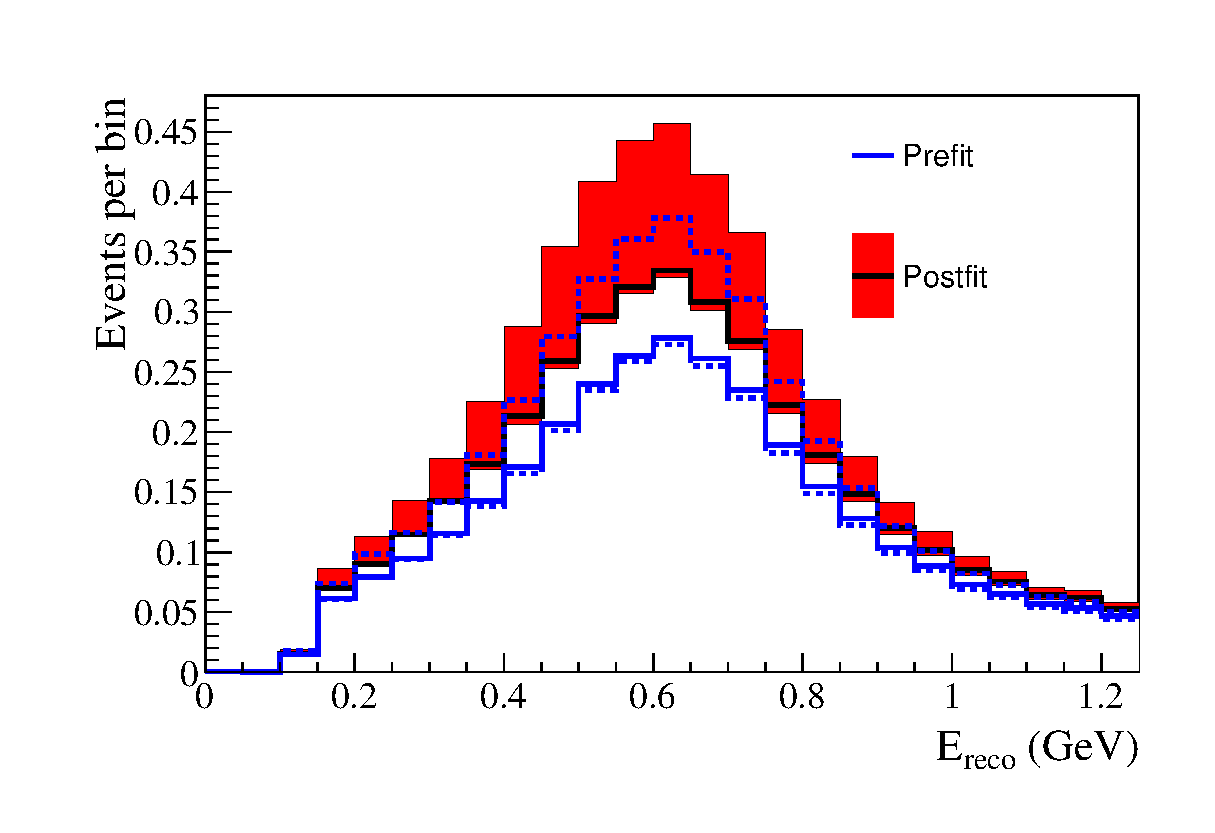
\includegraphics[width=18pc]{./nuebar_plots/spectrum_tweaked/oscillated_Osc_param_envelope.eps} % 1Rmu
%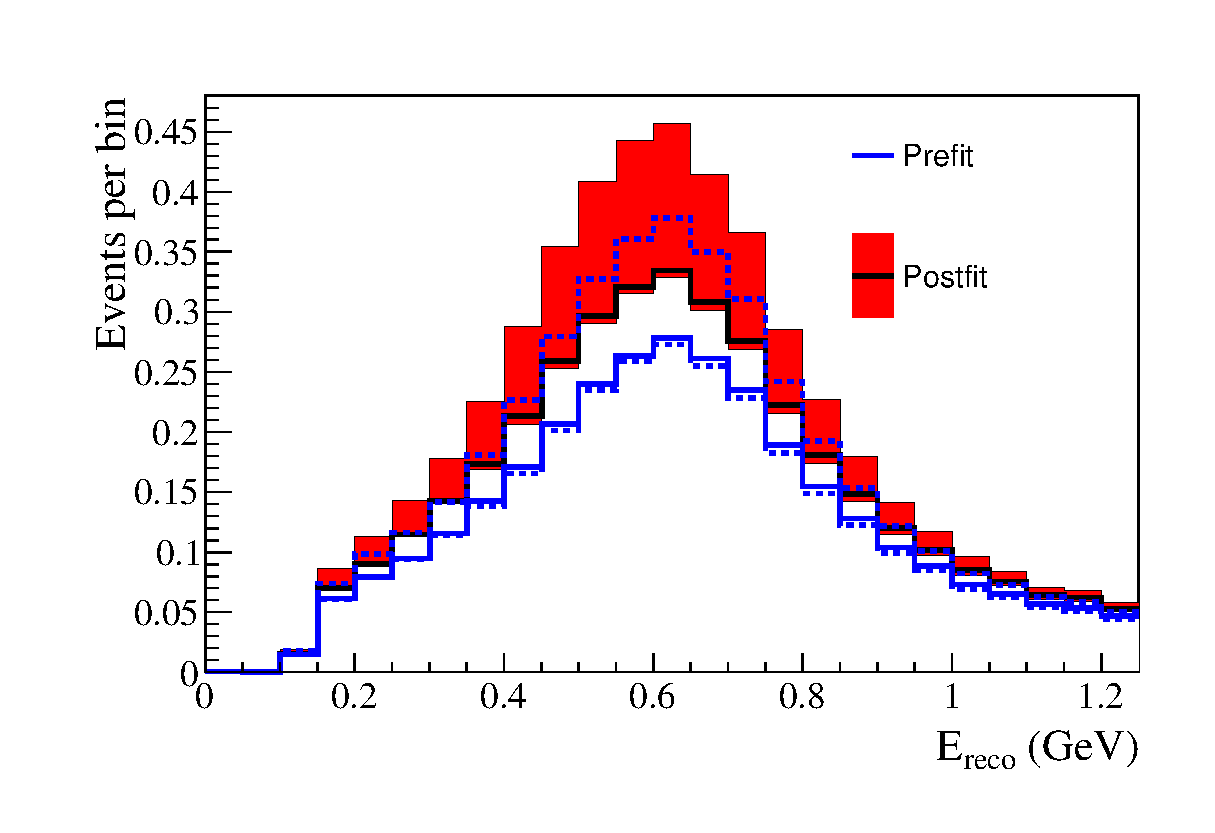
\includegraphics[width=18pc]{./nuebar_plots/spectrum_tweaked/oscillated_Osc_param_envelope.eps}\\ % RHCRmu
%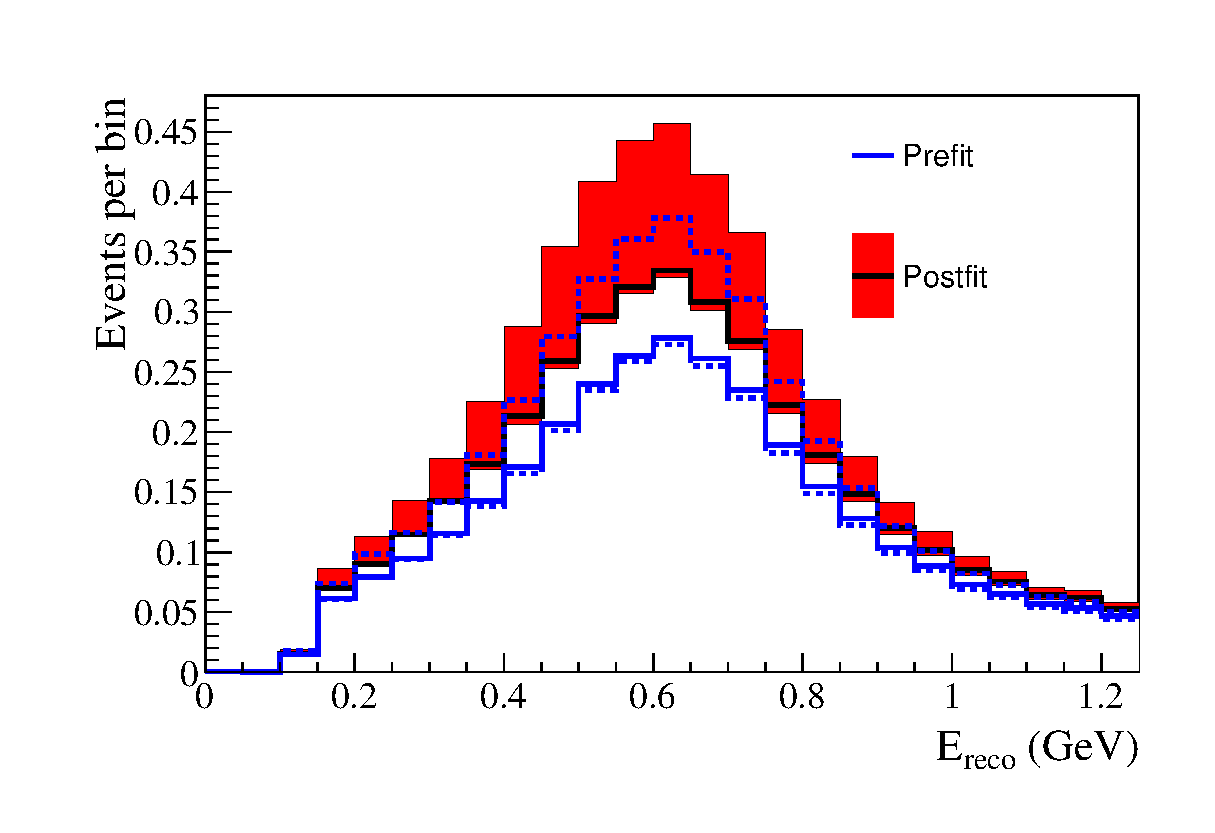
\includegraphics[width=18pc]{./nuebar_plots/spectrum_tweaked/oscillated_Osc_param_envelope.eps} % 1Re
%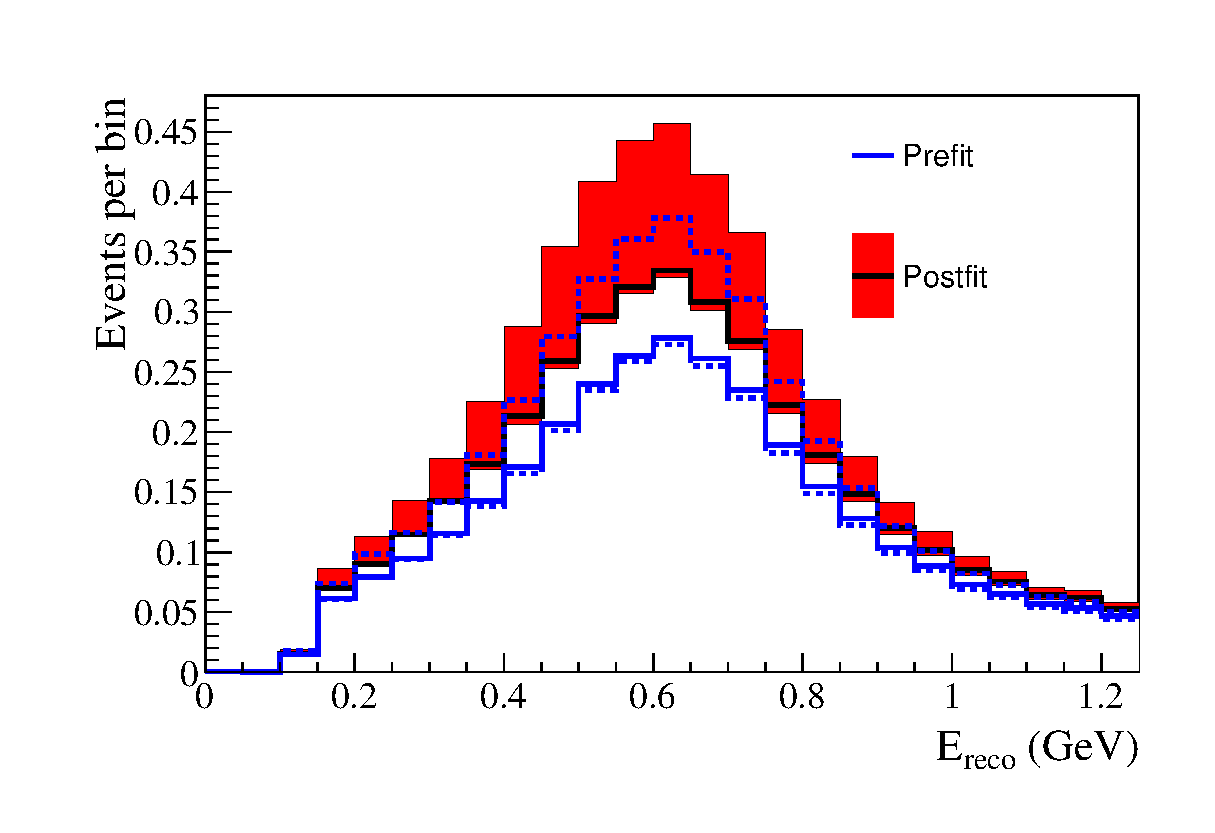
\includegraphics[width=18pc]{./nuebar_plots/spectrum_tweaked/oscillated_Osc_param_envelope.eps}\\ % RHCRe
%\caption {
%    \huge{TO UPDATE} % caption is already ok
%%  Error envelopes for the energy spectrum as a result of oscillation parameters
%%  for an exposure 
%%  of \TotalPotNu POT in neutrino mode
%%  and
%%  of \TotalPotNuBar POT in antineutrino mode.
%%  From top left to bottom right the following samples are shown:
%%  $\mu$-like neutrino mode,
%%  $\mu$-like antineutrino mode,
%%  $e$-like neutrino mode
%%  and 
%%  $e$-like antineutrino mode.
%%  \NumToys toy MC experiments were generated with randomized systematic parameters 
%%  and the 1$\sigma$ spread of bin contents was calculated.
%%  BANFF tuned MC templates were used.
%%  Existing correlations between the systematic parameters were taken into account.
%%  The error envelopes in each bin correspond to the $1\sigma$ error 
%%  obtained from the distribution of the extracted number of events.
%%  First the median is found. 
%%  Then the upper (lower) error corresponds
%%  to the number of events for which the 34\% of toys is contained
%%  in the right (left) side of the median.
%%  The continuos line shows the expected nominal reconstructed energy distribution 
%%  for pre-BANFF (blue) and post-BANFF (black).
%%  The oscillation parameters shown in Tab.~\ref{tab:osc_params_joint} are used.
%}
%\label{fig:Osc_envelope}
%\end{figure*}
%
%
%\begin{figure*}[htb]
%\center
%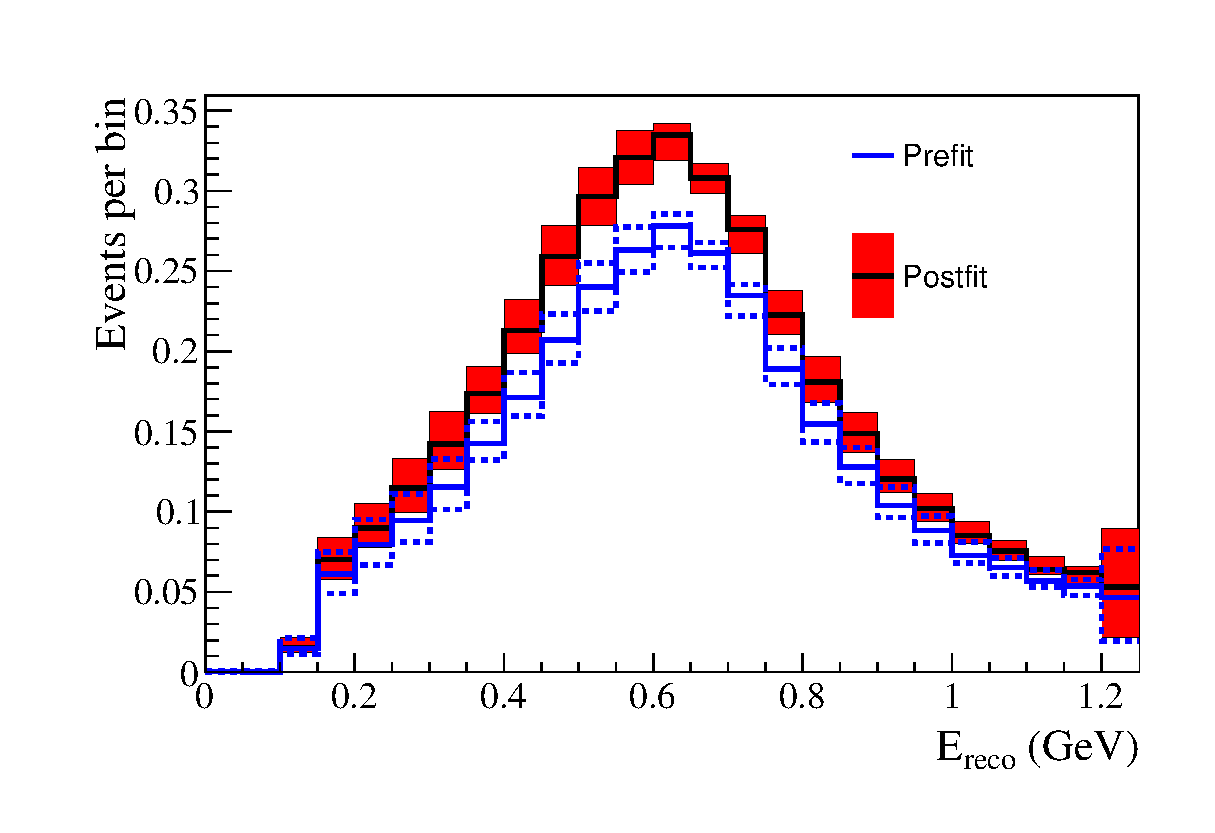
\includegraphics[width=18pc]{./nuebar_plots/spectrum_tweaked/oscillated_SKDet_FSI_envelope.eps} % 1Rmu
%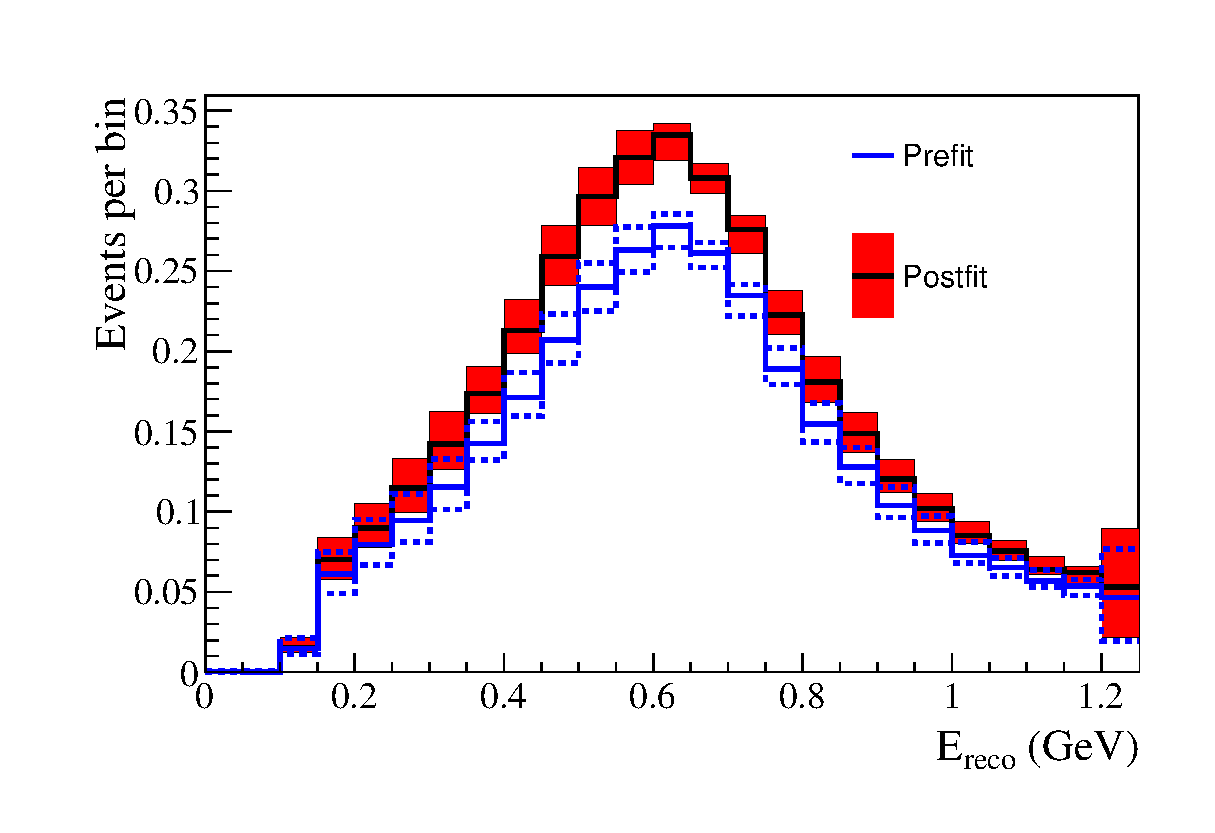
\includegraphics[width=18pc]{./nuebar_plots/spectrum_tweaked/oscillated_SKDet_FSI_envelope.eps}\\ % RHC1Rmu
%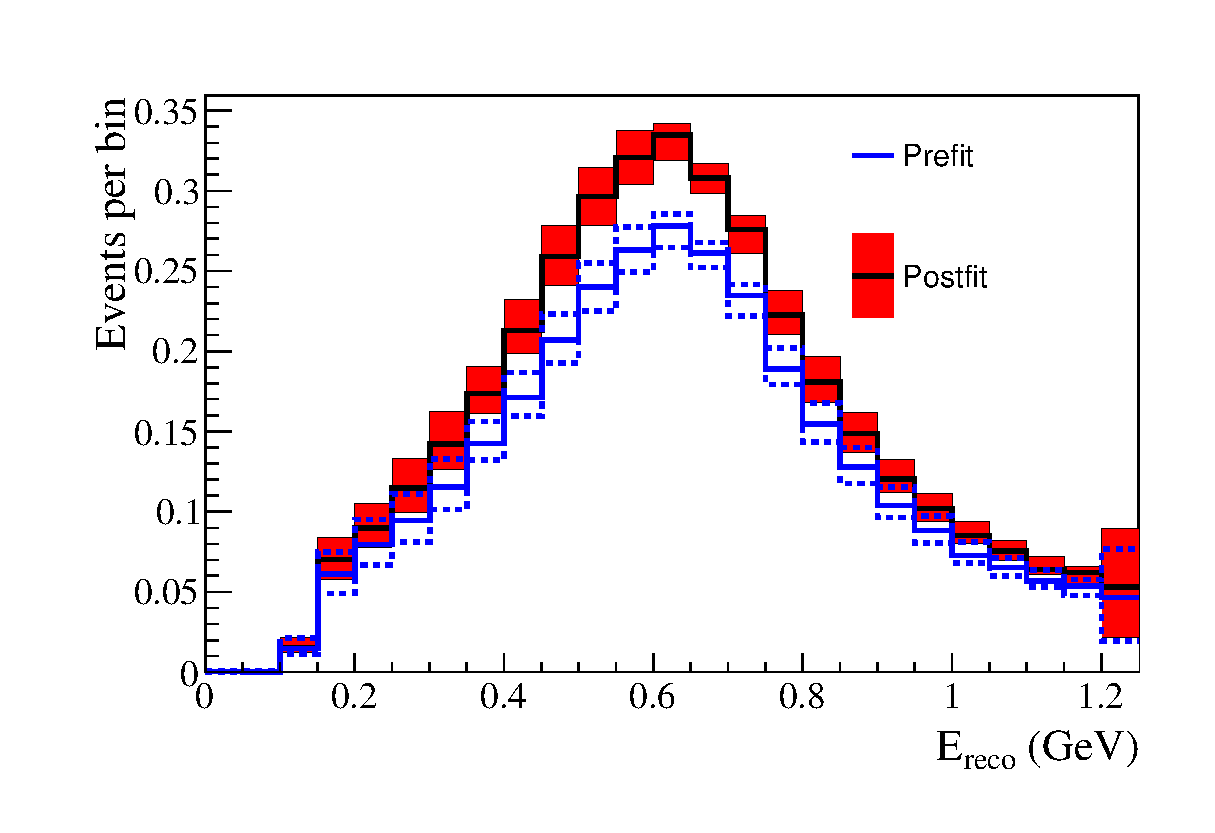
\includegraphics[width=18pc]{./nuebar_plots/spectrum_tweaked/oscillated_SKDet_FSI_envelope.eps} % 1Re
%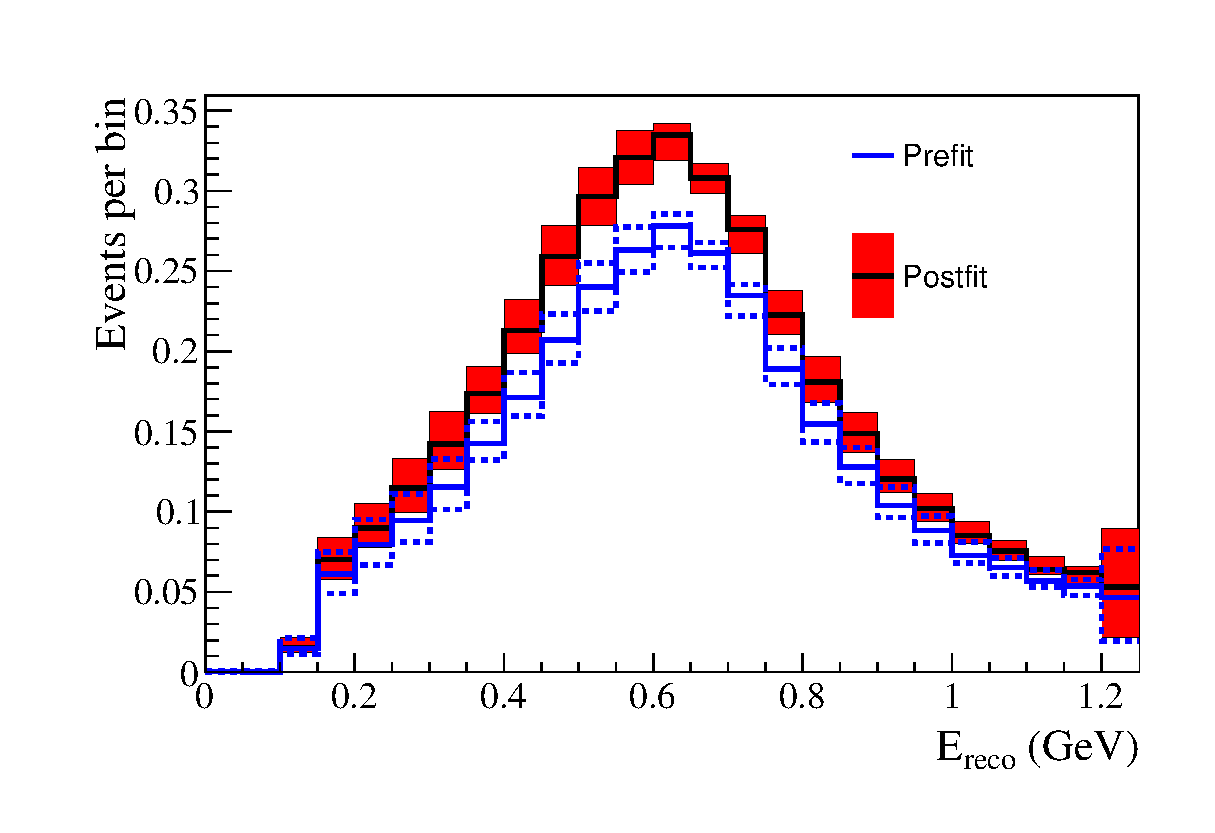
\includegraphics[width=18pc]{./nuebar_plots/spectrum_tweaked/oscillated_SKDet_FSI_envelope.eps}\\ % RHC1Re
%\caption {
%    \huge{TO UPDATE} % caption is already ok
%%  Error envelopes for the energy spectrum as a result of Super-K detector and FSI/SI parameters
%%    for an exposure 
%%  of \TotalPotNu POT in neutrino mode
%%  and
%%  of \TotalPotNuBar POT in antineutrino mode.
%%     From top left to bottom right the following samples are shown:
%%  $\mu$-like neutrino mode,
%%  $\mu$-like antineutrino mode,
%%  $e$-like neutrino mode
%%  and 
%%  $e$-like antineutrino mode.
%%  \NumToys toy MC experiments were generated with randomized systematic parameters and 
%%  the 1$\sigma$ spread of bin contents was calculated.
%%  BANFF tuned MC templates were used.
%%  Existing correlations between the systematic parameters were taken into account.
%%  The error envelopes in each bin correspond to the $1\sigma$ error 
%%  obtained from the distribution of the extracted number of events.
%%  First the median (red line) is found. 
%%  Then the upper (lower) error corresponds
%%  to the number of events for which the 34\% of toys is contained
%%  in the right (left) side of the median.
%%  The continuos line shows the expected nominal reconstructed energy distribution 
%%  for pre-BANFF (blue) and post-BANFF (black).
%%    The oscillation parameters shown in Tab.~\ref{tab:osc_params_joint} are used.
%}
%\label{fig:SKDet_FSI_envelope}
%\end{figure*}
%
%\begin{figure*}[htb]
%\center
%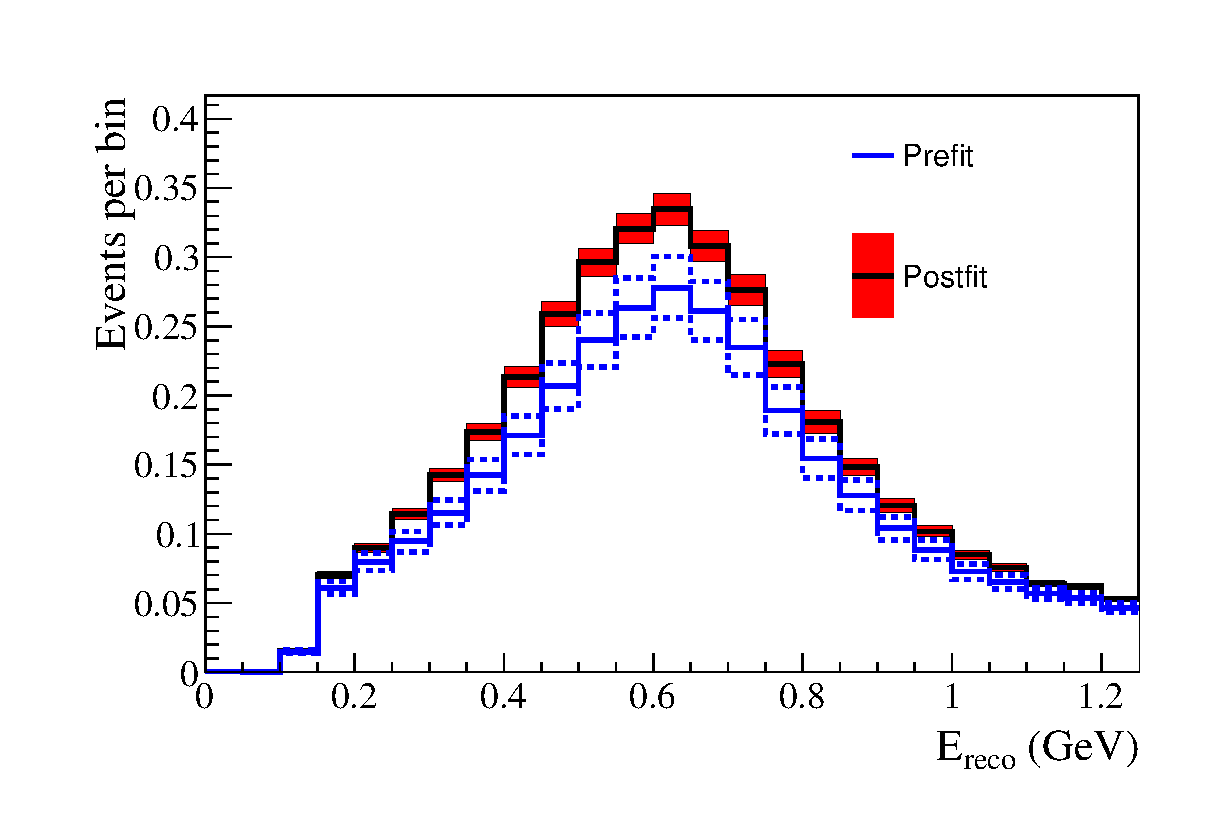
\includegraphics[width=18pc]{./nuebar_plots/spectrum_tweaked/oscillated_BANFF_flux_envelope.eps} % 1Rmu
%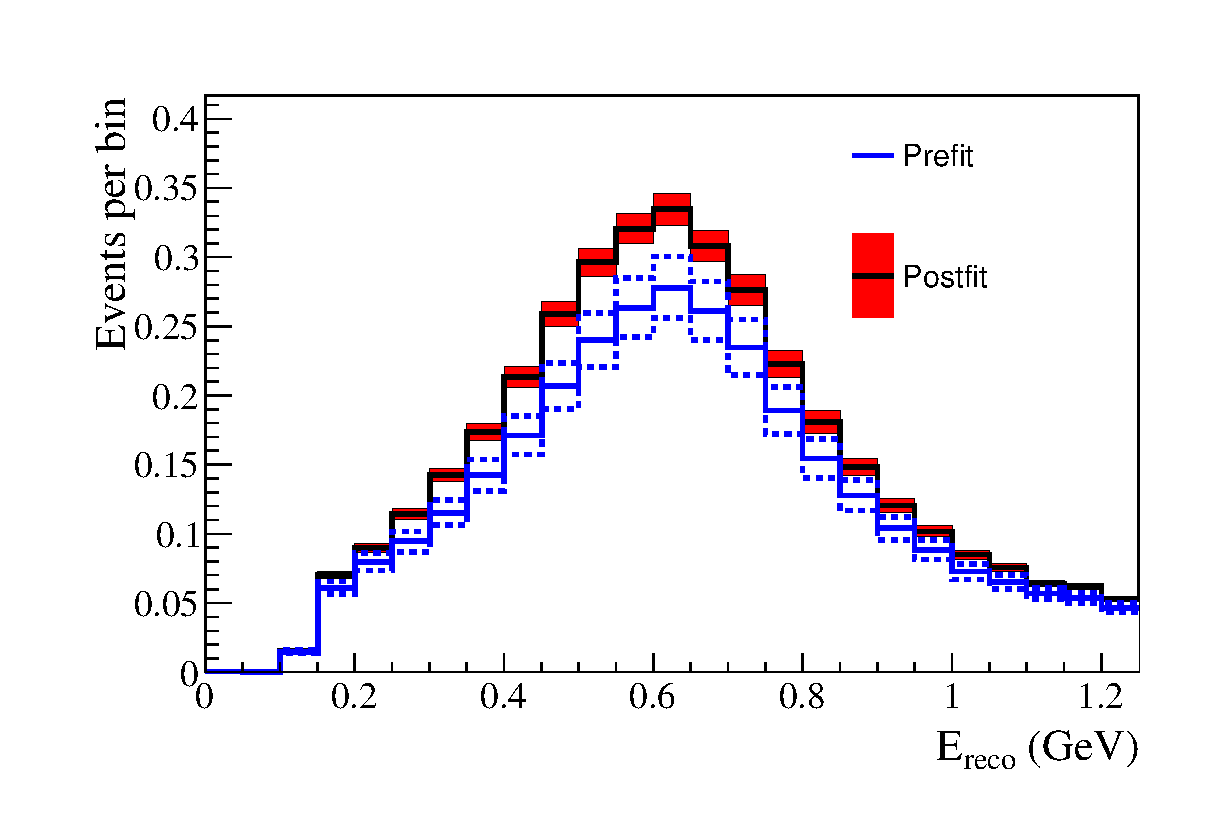
\includegraphics[width=18pc]{./nuebar_plots/spectrum_tweaked/oscillated_BANFF_flux_envelope.eps}\\ % RHC1Rmu
%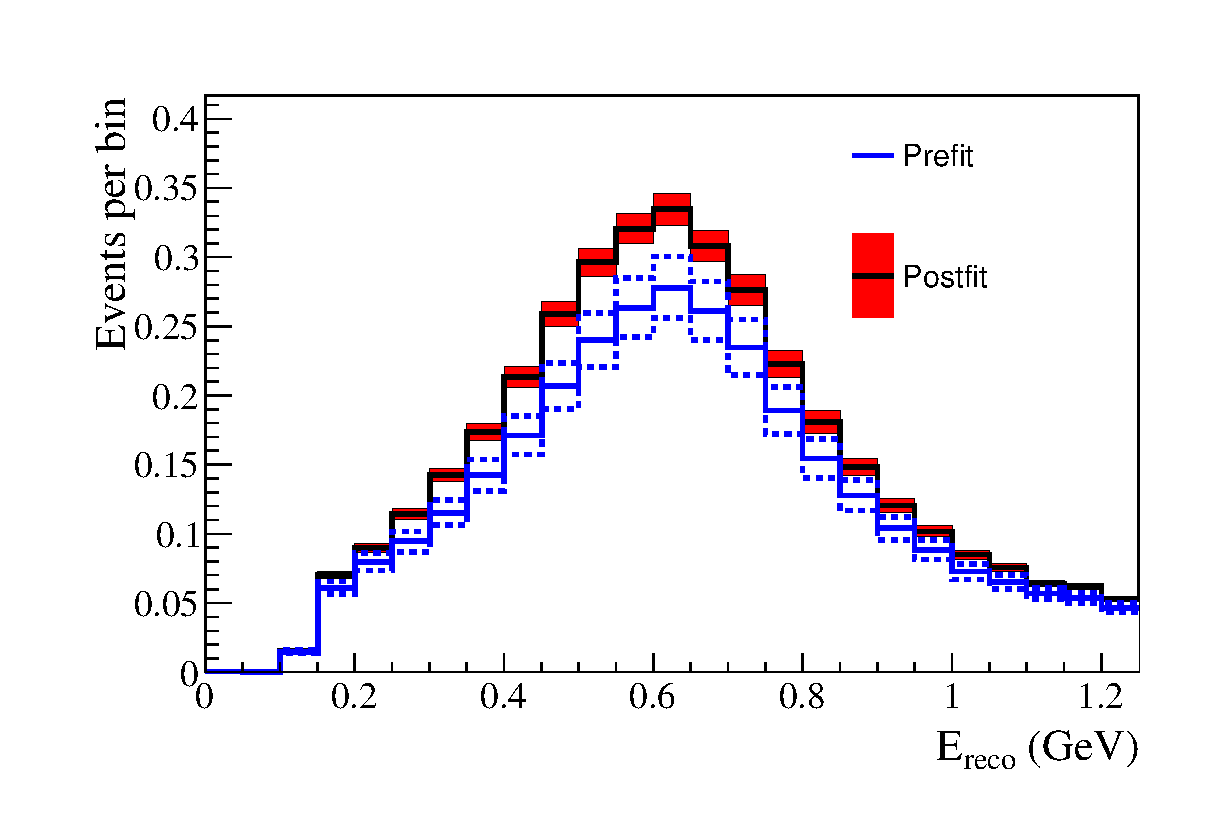
\includegraphics[width=18pc]{./nuebar_plots/spectrum_tweaked/oscillated_BANFF_flux_envelope.eps} % 1Re
%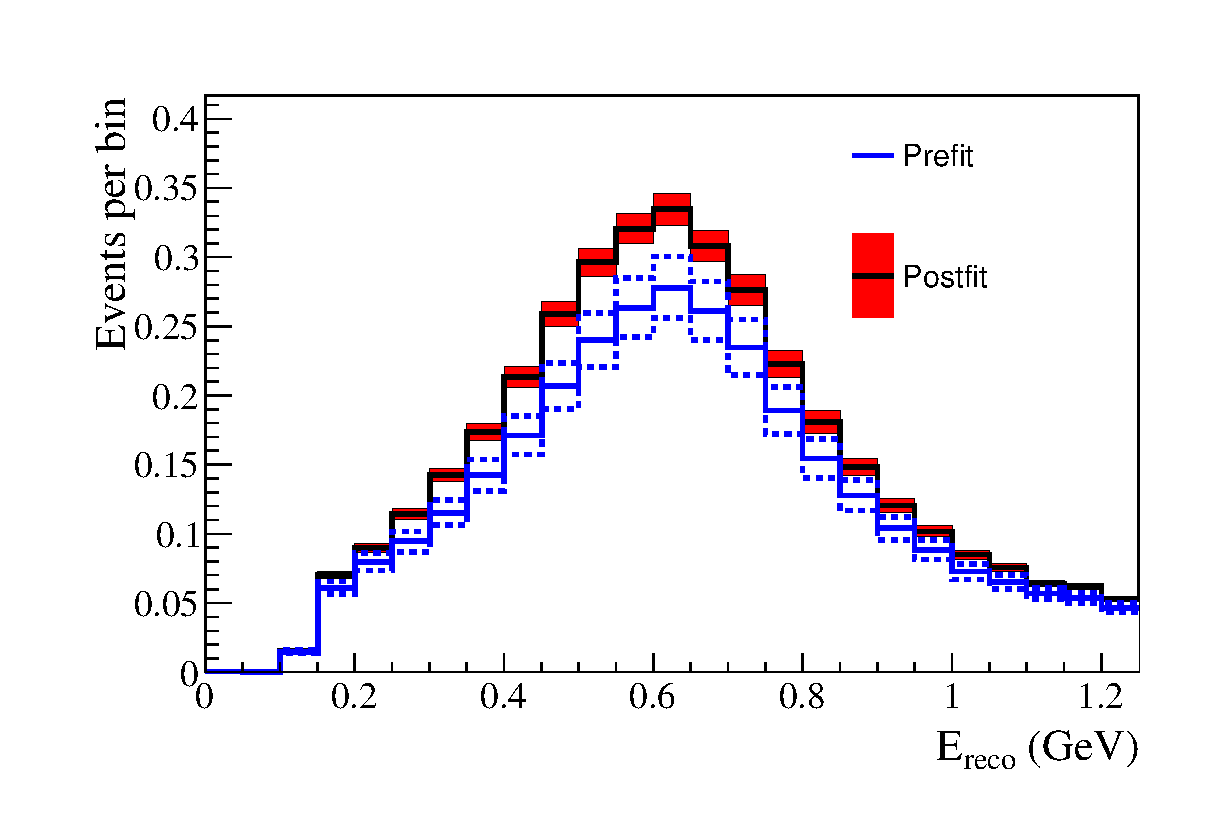
\includegraphics[width=18pc]{./nuebar_plots/spectrum_tweaked/oscillated_BANFF_flux_envelope.eps}\\ % RHC1Re
%\caption {
%    \huge{TO UPDATE} % caption is already ok
%%  Error envelopes for the energy spectrum as a result of flux systematics
%%    for an exposure 
%%  of \TotalPotNu POT in neutrino mode
%%  and
%%  of \TotalPotNuBar POT in antineutrino mode.
%%   From top left to bottom right the following samples are shown:
%%  $\mu$-like neutrino mode,
%%  $\mu$-like antineutrino mode,
%%  $e$-like neutrino mode
%%  and 
%%  $e$-like antineutrino mode.
%%  \NumToys toy MC experiments were generated with randomized systematic parameters and the 1$\sigma$ spread of bin contents was calculated.
%%  BANFF tuned MC templates were used.
%%  Existing correlations between the systematic parameters were taken into account.
%%  The error envelopes in each bin correspond to the $1\sigma$ error 
%%  obtained from the distribution of the extracted number of events.
%%  First the median (red line) is found. 
%%  Then the upper (lower) error corresponds
%%  to the number of events for which the 34\% of toys is contained
%%  in the right (left) side of the median.
%%  The continuos line shows the expected nominal reconstructed energy distribution 
%%  for pre-BANFF (blue) and post-BANFF (black).
%%    The oscillation parameters shown in Tab.~\ref{tab:osc_params_joint} are used.
%}
%\label{fig:flux_envelope}
%\end{figure*}
%
%\begin{figure*}[htb]
%\center
%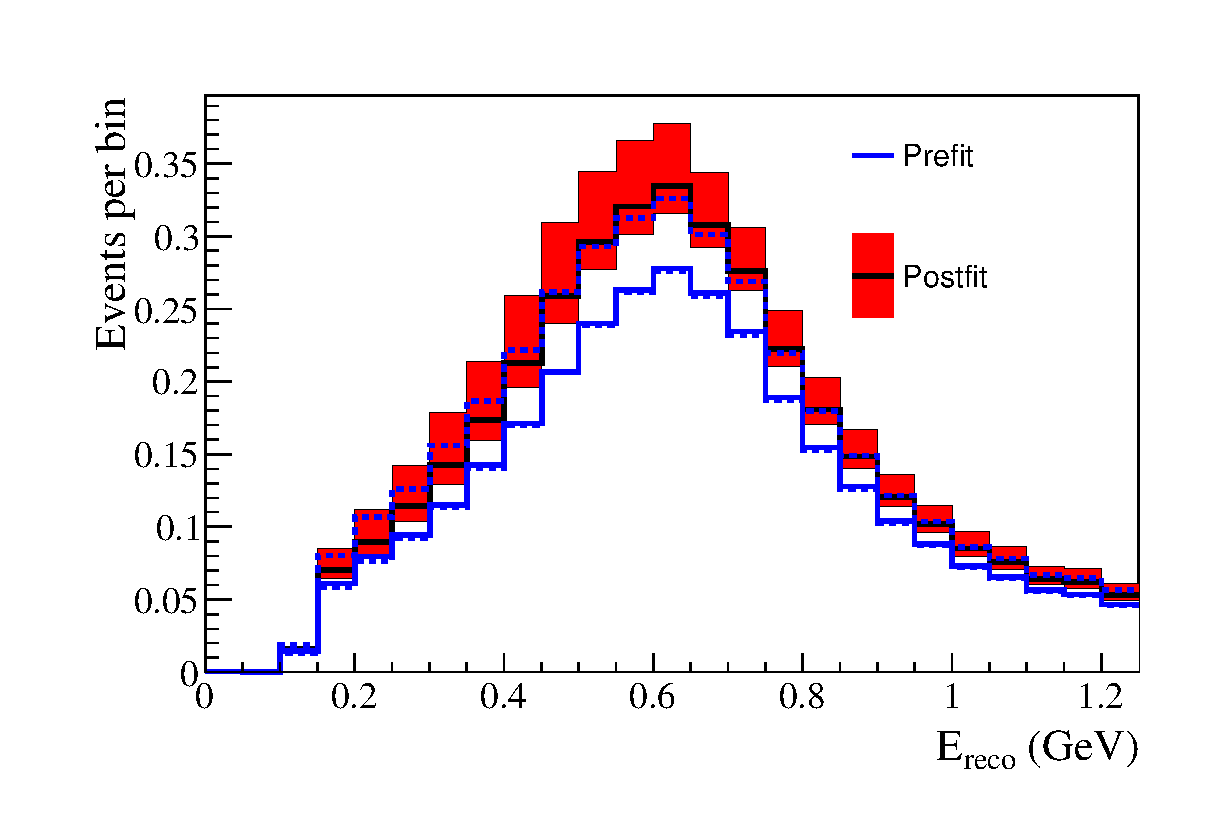
\includegraphics[width=18pc]{./nuebar_plots/spectrum_tweaked/oscillated_BANFF_xsec_envelope.eps} % 1Rmu
%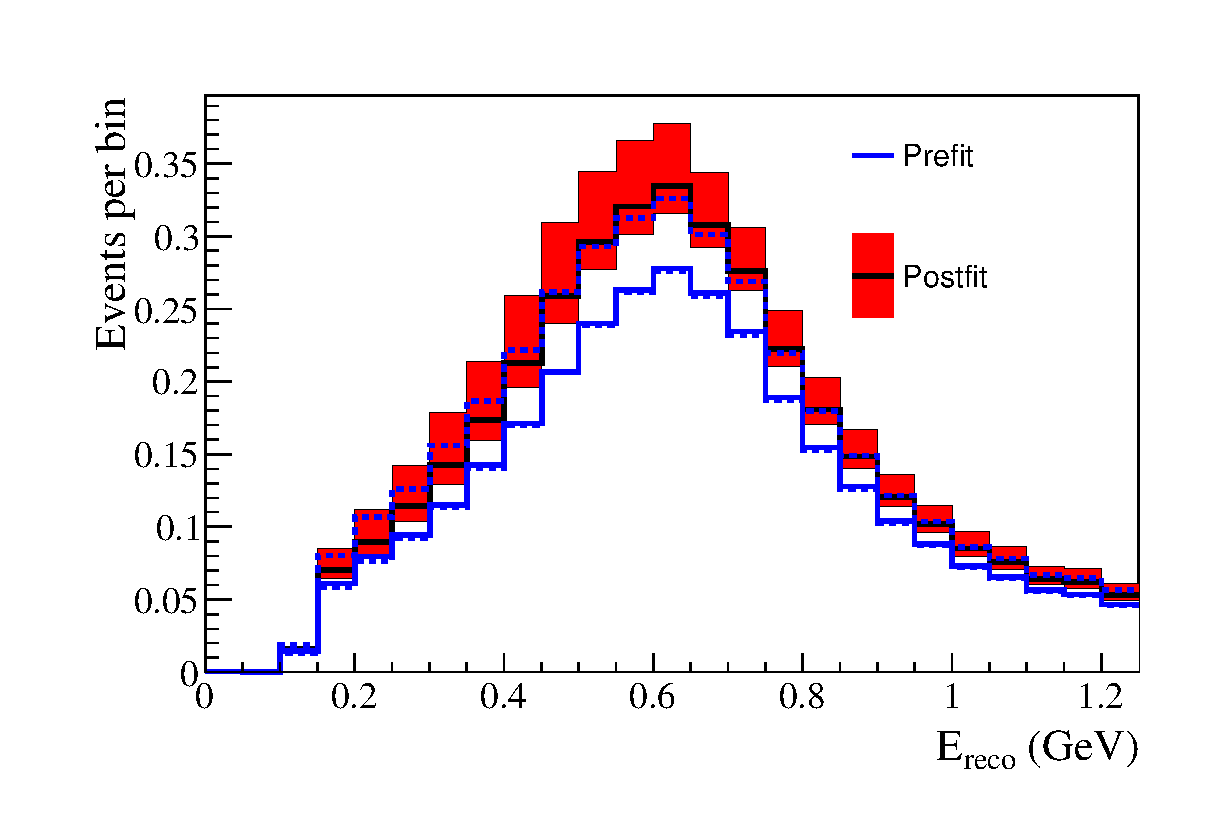
\includegraphics[width=18pc]{./nuebar_plots/spectrum_tweaked/oscillated_BANFF_xsec_envelope.eps}\\ % RHC1Rmu
%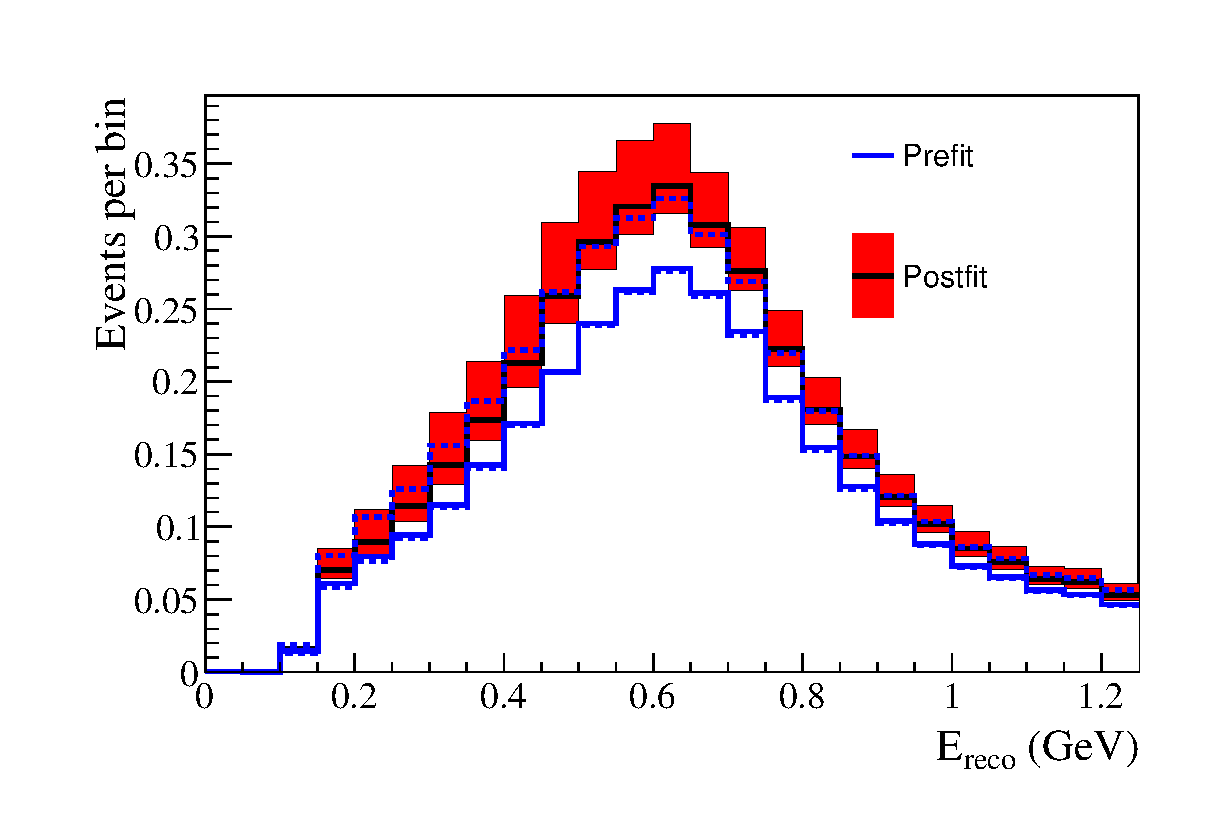
\includegraphics[width=18pc]{./nuebar_plots/spectrum_tweaked/oscillated_BANFF_xsec_envelope.eps} % 1Re
%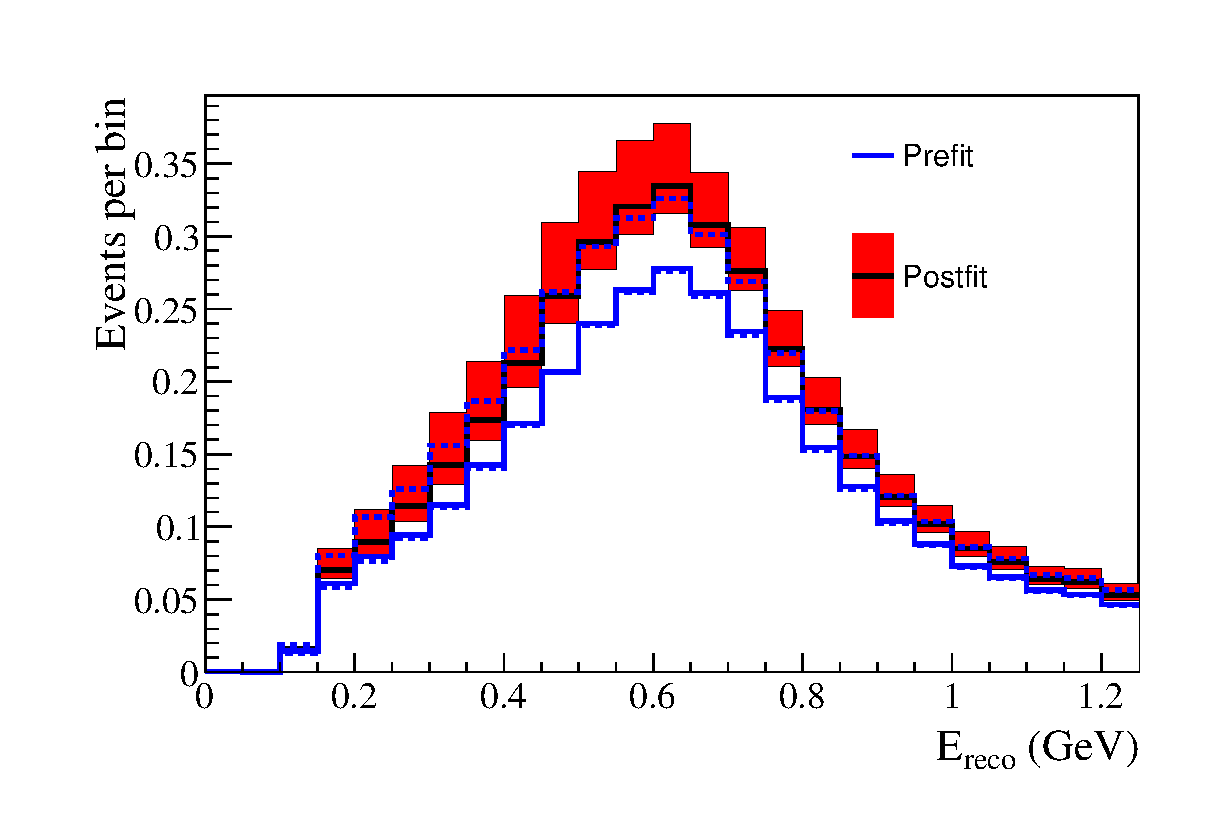
\includegraphics[width=18pc]{./nuebar_plots/spectrum_tweaked/oscillated_BANFF_xsec_envelope.eps}\\ % RHC1Re
%\caption {
%    \huge{TO UPDATE} % caption is already ok
%%  Error envelopes for the energy spectrum as a result of only cross-section parameters
%%    for an exposure 
%%  of \TotalPotNu POT in neutrino mode
%%  and
%%  of \TotalPotNuBar POT in antineutrino mode.
%%    From top left to bottom right the following samples are shown:
%%  $\mu$-like neutrino mode,
%%  $\mu$-like antineutrino mode,
%%  $e$-like neutrino mode
%%  and 
%%  $e$-like antineutrino mode.
%%  \NumToys toy MC experiments were generated with randomized systematic parameters and 
%%  the 1$\sigma$ spread of bin contents was calculated.
%%  BANFF tuned MC templates were used.
%%  Existing correlations between the systematic parameters were taken into account.
%%  The error envelopes in each bin correspond to the $1\sigma$ error 
%%  obtained from the distribution of the extracted number of events.
%%  First the median (red line) is found. 
%%  Then the upper (lower) error corresponds
%%  to the number of events for which the 34\% of toys is contained
%%  in the right (left) side of the median.
%%  The continuos line shows the expected nominal reconstructed energy distribution 
%%  for pre-BANFF (blue) and post-BANFF (black).
%%  The oscillation parameters shown in Tab.~\ref{tab:osc_params_joint} are used.
%}
%\label{fig:xsec_envelope}
%\end{figure*}
%
%\begin{figure*}[htb]
%\center
%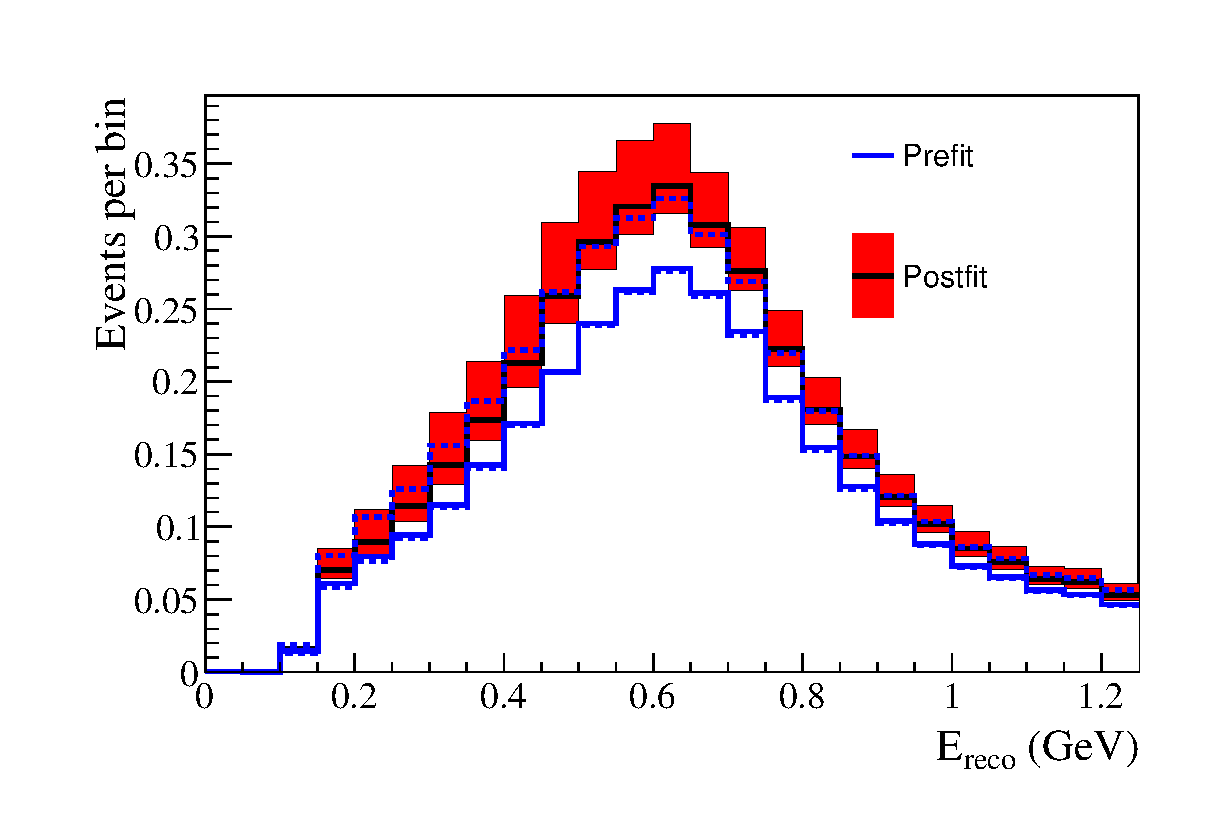
\includegraphics[width=18pc]{./nuebar_plots/spectrum_tweaked/oscillated_BANFF_xsec_envelope.eps} % 1Rmu
%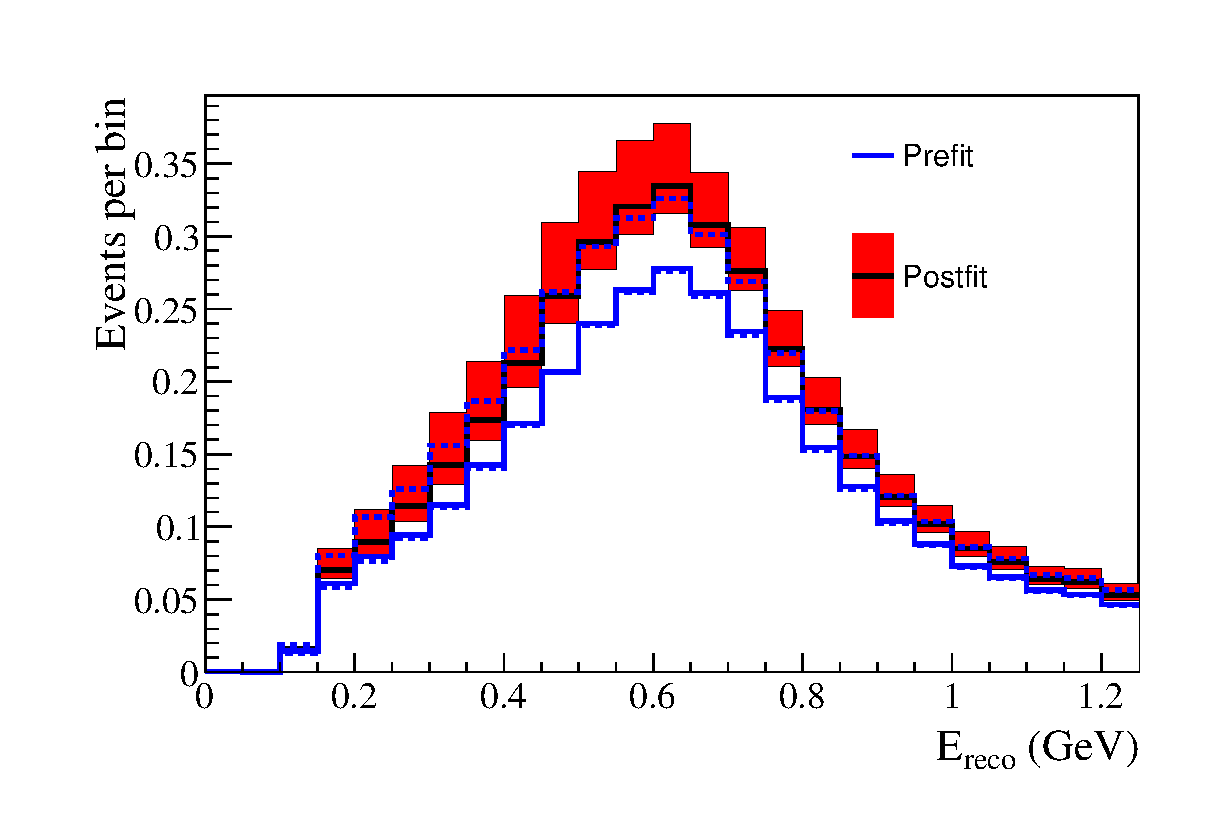
\includegraphics[width=18pc]{./nuebar_plots/spectrum_tweaked/oscillated_BANFF_xsec_envelope.eps}\\ % RHC1Rmu
%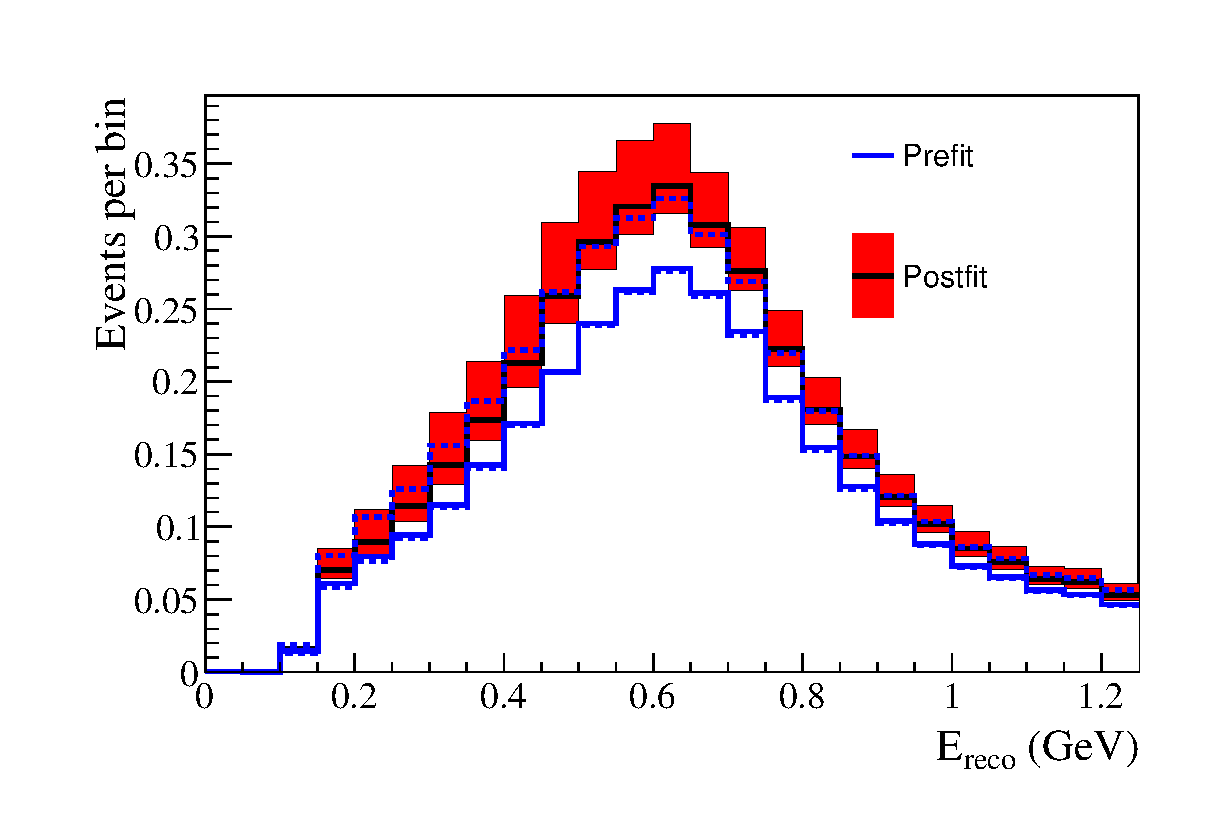
\includegraphics[width=18pc]{./nuebar_plots/spectrum_tweaked/oscillated_BANFF_xsec_envelope.eps} % 1Re
%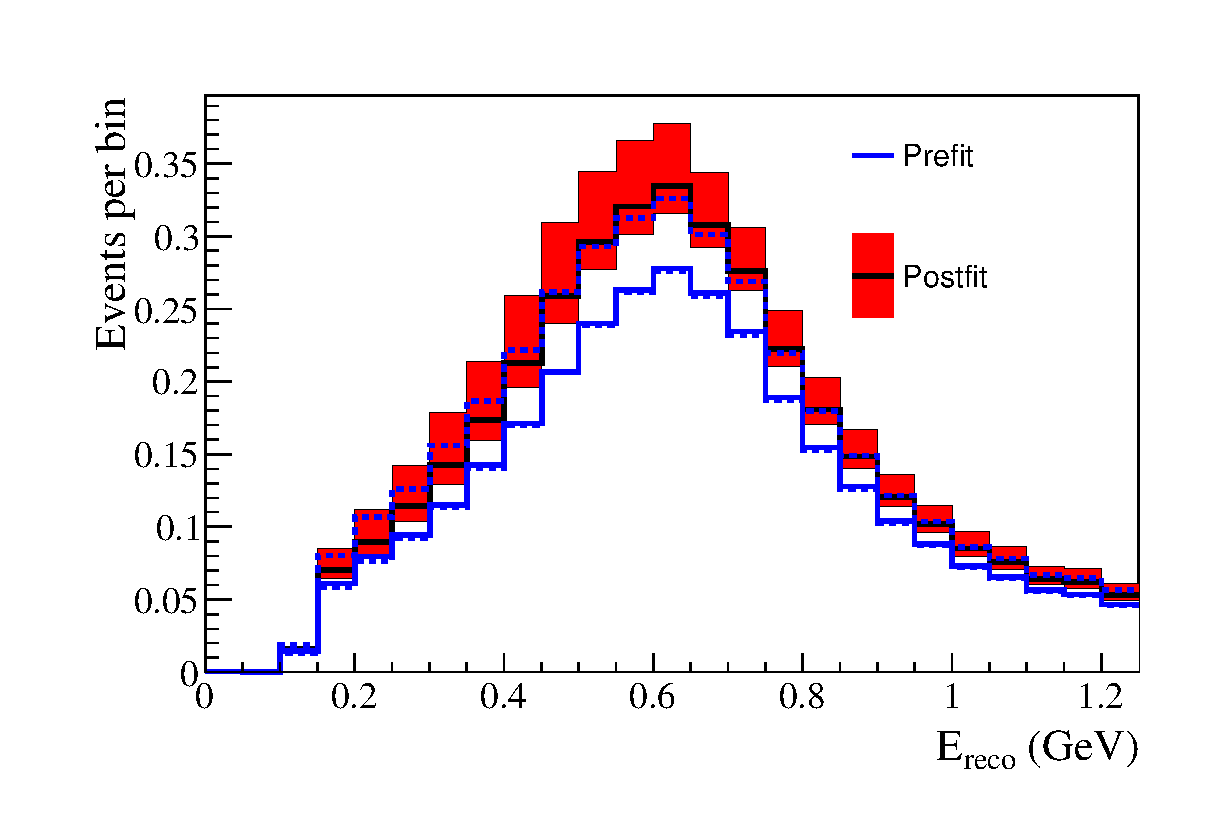
\includegraphics[width=18pc]{./nuebar_plots/spectrum_tweaked/oscillated_BANFF_xsec_envelope.eps}\\ % RHC1Re
%\caption {
%    \huge{TO UPDATE} % caption is already ok
%%  Error envelopes for the energy spectrum as a result of only flux and cross-section parameters
%%    for an exposure 
%%  of \TotalPotNu POT in neutrino mode
%%  and
%%  of \TotalPotNuBar POT in antineutrino mode.
%%    From top left to bottom right the following samples are shown:
%%  $\mu$-like neutrino mode,
%%  $\mu$-like antineutrino mode,
%%  $e$-like neutrino mode
%%  and 
%%  $e$-like antineutrino mode.
%%  \NumToys toy MC experiments were generated with randomized systematic parameters and 
%%  the 1$\sigma$ spread of bin contents was calculated.
%%  BANFF tuned MC templates were used.
%%  Existing correlations between the systematic parameters were taken into account.
%%  The error envelopes in each bin correspond to the $1\sigma$ error 
%%  obtained from the distribution of the extracted number of events.
%%  First the median (red line) is found. 
%%  Then the upper (lower) error corresponds
%%  to the number of events for which the 34\% of toys is contained
%%  in the right (left) side of the median.
%%  The continuos line shows the expected nominal reconstructed energy distribution 
%%  for pre-BANFF (blue) and post-BANFF (black).
%%  The oscillation parameters shown in Tab.~\ref{tab:osc_params_joint} are used.
%}
%\label{fig:flux_xsec_envelope}
%\end{figure*}
%
%\begin{figure*}[htb]
%\center
%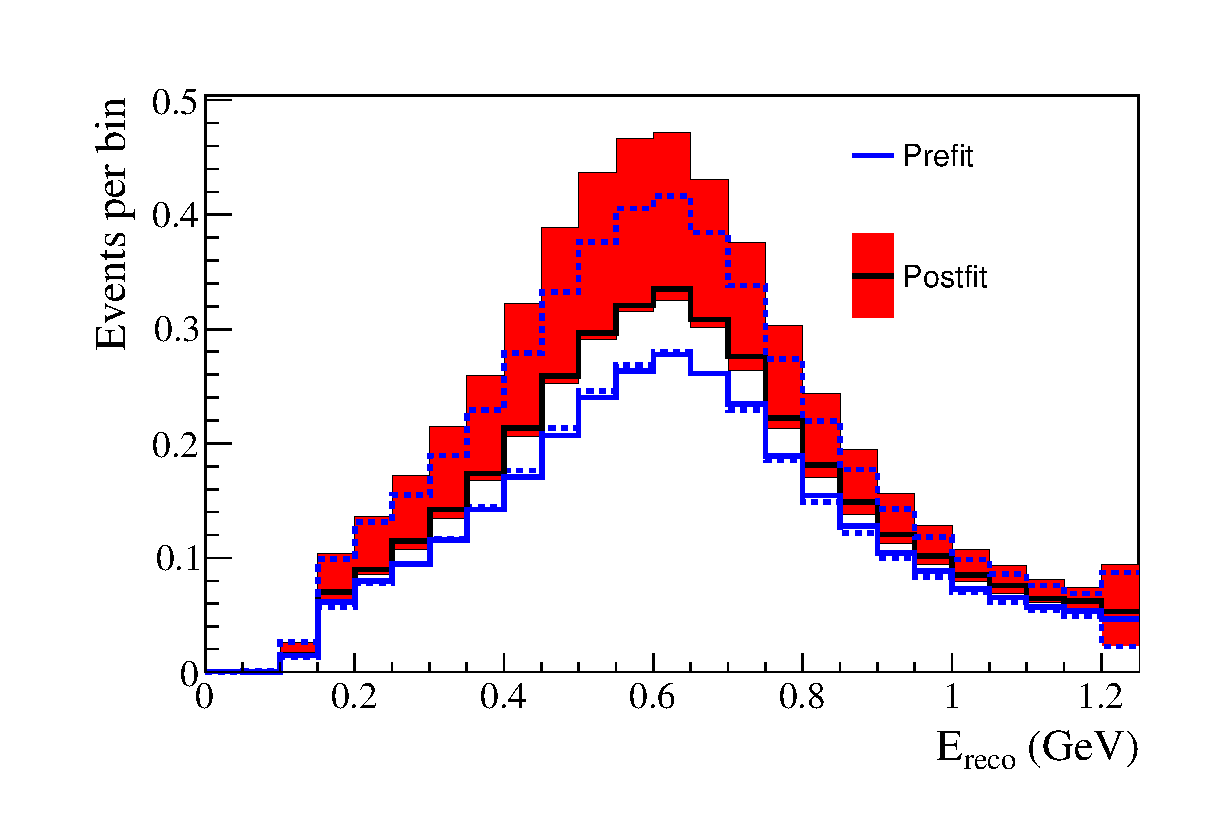
\includegraphics[width=18pc]{./nuebar_plots/spectrum_tweaked/oscillated_all_envelope.eps} % 1Rmu
%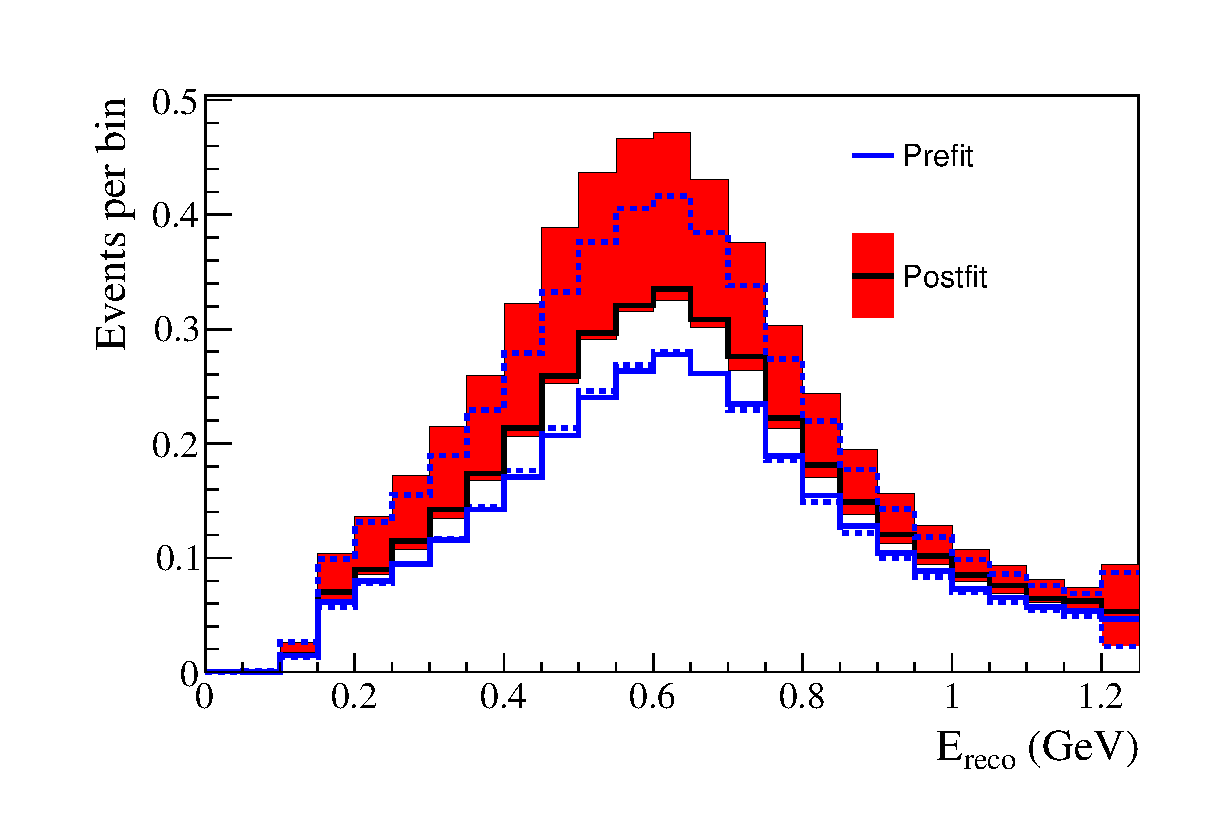
\includegraphics[width=18pc]{./nuebar_plots/spectrum_tweaked/oscillated_all_envelope.eps}\\ % RHC1Rmu
%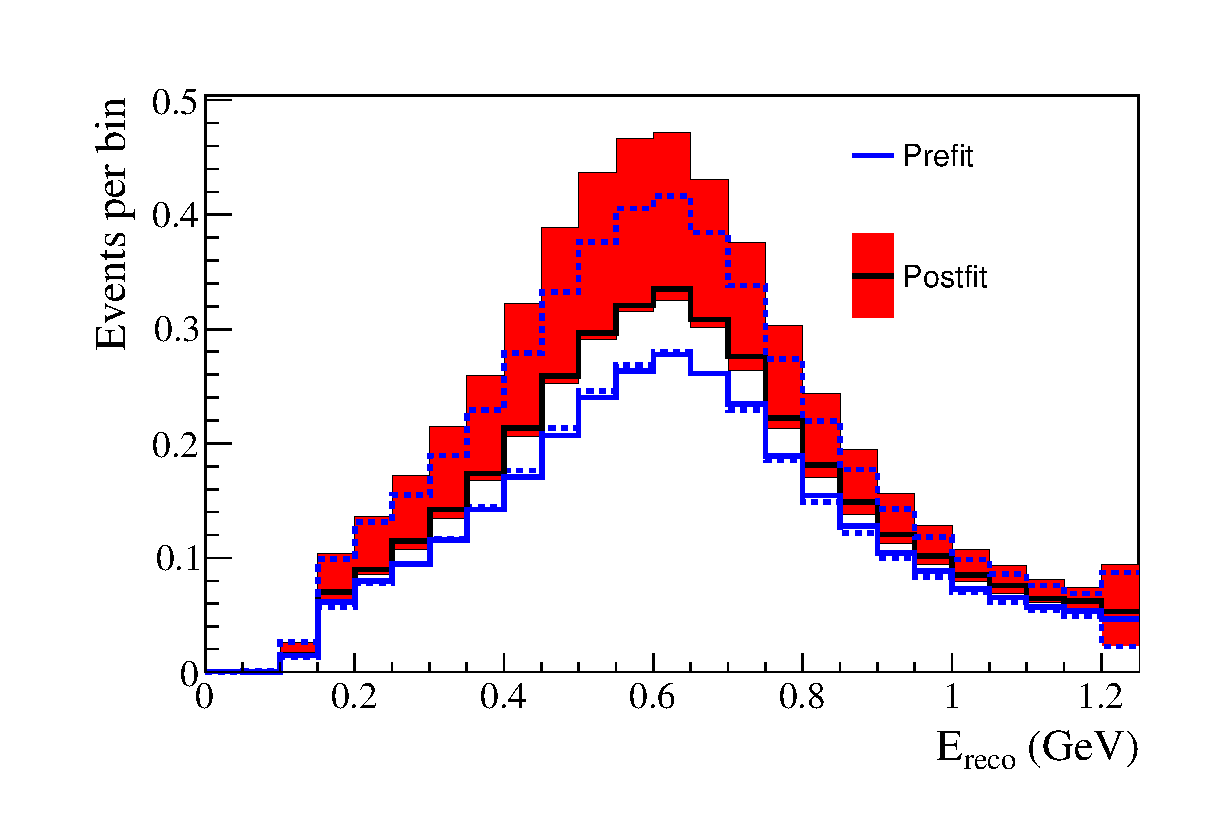
\includegraphics[width=18pc]{./nuebar_plots/spectrum_tweaked/oscillated_all_envelope.eps} % 1Re
%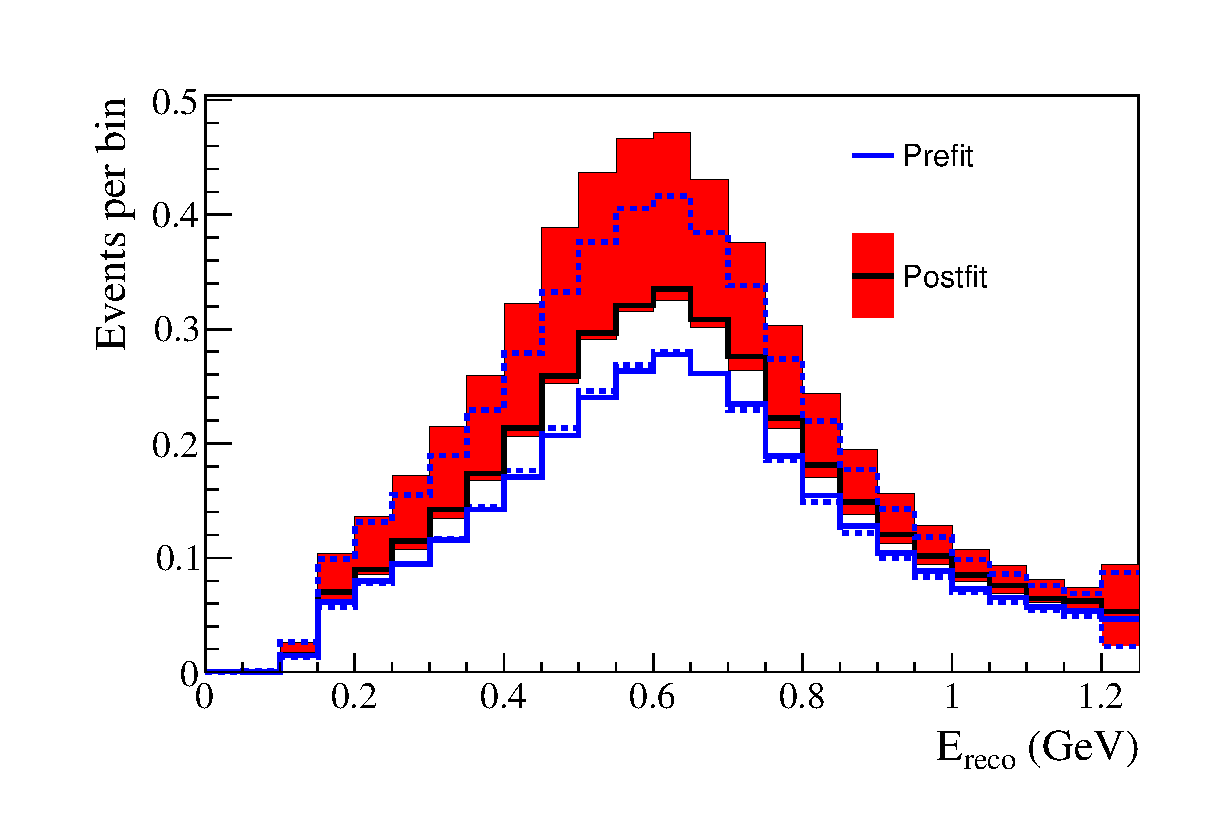
\includegraphics[width=18pc]{./nuebar_plots/spectrum_tweaked/oscillated_all_envelope.eps}\\ % RHC1Re
%\caption {
%    \huge{TO UPDATE} % caption is already ok
%%  Error envelopes for the energy spectrum as a result of all systematic parameters
%%    for an exposure 
%%  of \TotalPotNu POT in neutrino mode
%%  and
%%  of \TotalPotNuBar POT in antineutrino mode.
%%  From top left to bottom right the following samples are shown:
%%  $\mu$-like neutrino mode,
%%  $\mu$-like antineutrino mode,
%%  $e$-like neutrino mode
%%  and 
%%  $e$-like antineutrino mode.
%%  \NumToys toy MC experiments were generated with randomized systematic parameters and the 1$\sigma$ spread of bin contents was calculated.
%%  BANFF tuned MC templates were used.
%%  Existing correlations between the systematic parameters were taken into account.
%%  The error envelopes in each bin correspond to the $1\sigma$ error 
%%  obtained from the distribution of the extracted number of events.
%%  First the median (red line) is found. 
%%  Then the upper (lower) error corresponds
%%  to the number of events for which the 34\% of toys is contained
%%  in the right (left) side of the median.
%%  The continuos line shows the expected nominal reconstructed energy distribution 
%%  for pre-BANFF (blue) and post-BANFF (black).
%%  The oscillation parameters shown in Tab.~\ref{tab:osc_params_joint} are used.
%}
%\label{fig:all_envelope}
%\end{figure*}
%
%
%
%\clearpage
%
%
%
%
%%Ratio oscillated
%
%
%In Fig.~\ref{fig:Osc_envelope_ratio},~\ref{fig:SKDet_FSI_envelope_ratio},~\ref{fig:flux_envelope_ratio},
%\ref{fig:xsec_envelope_ratio},~\ref{fig:flux_xsec_envelope_ratio} and~\ref{fig:all_envelope_ratio}
%the ratio error envelopes of reconstructed energy spectra for all the selected samples,
%given respectively by
%oscillations, Super-K detector + FSI/SI, flux only, cross section only, flux+cross section and all the systematics
%are shown. 
%
%
%\begin{figure*}[htb]
%\center
%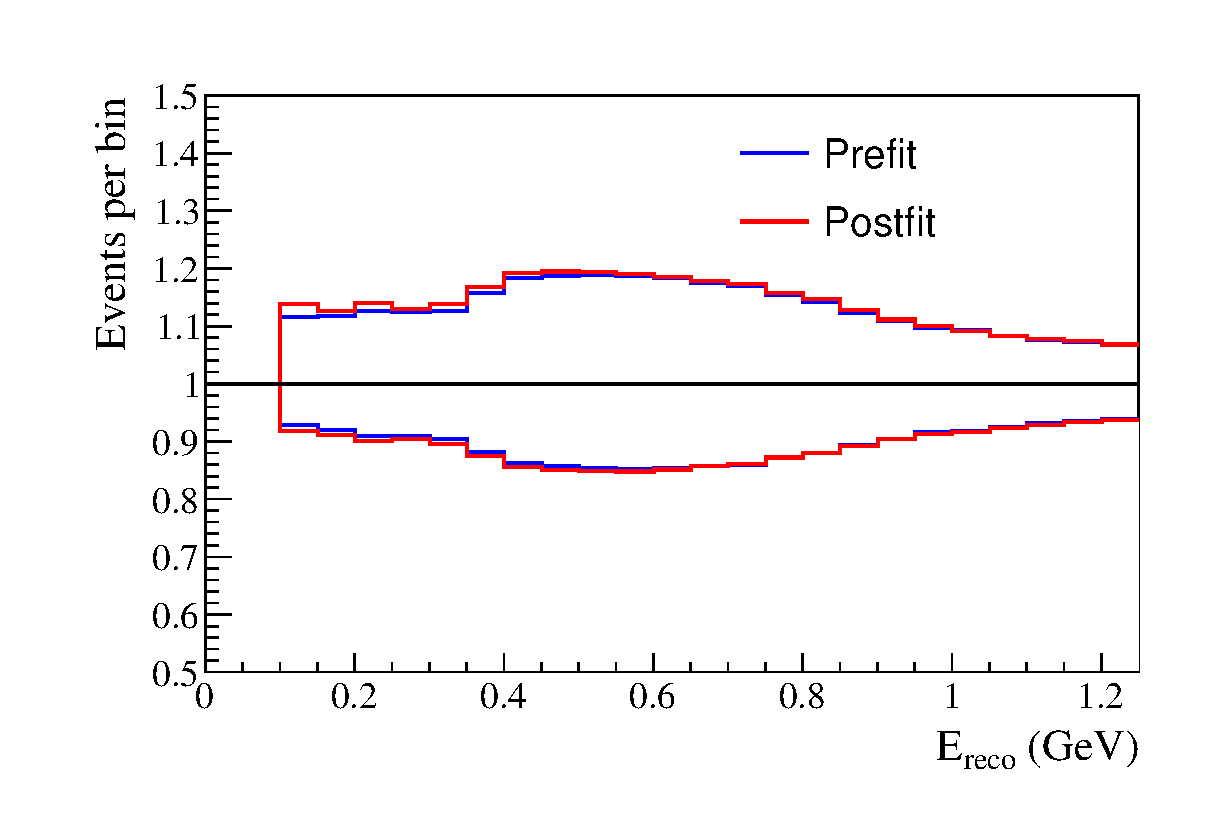
\includegraphics[width=18pc]{./nuebar_plots/spectrum_tweaked/oscillated_Osc_param_envelope_ratio.eps}
%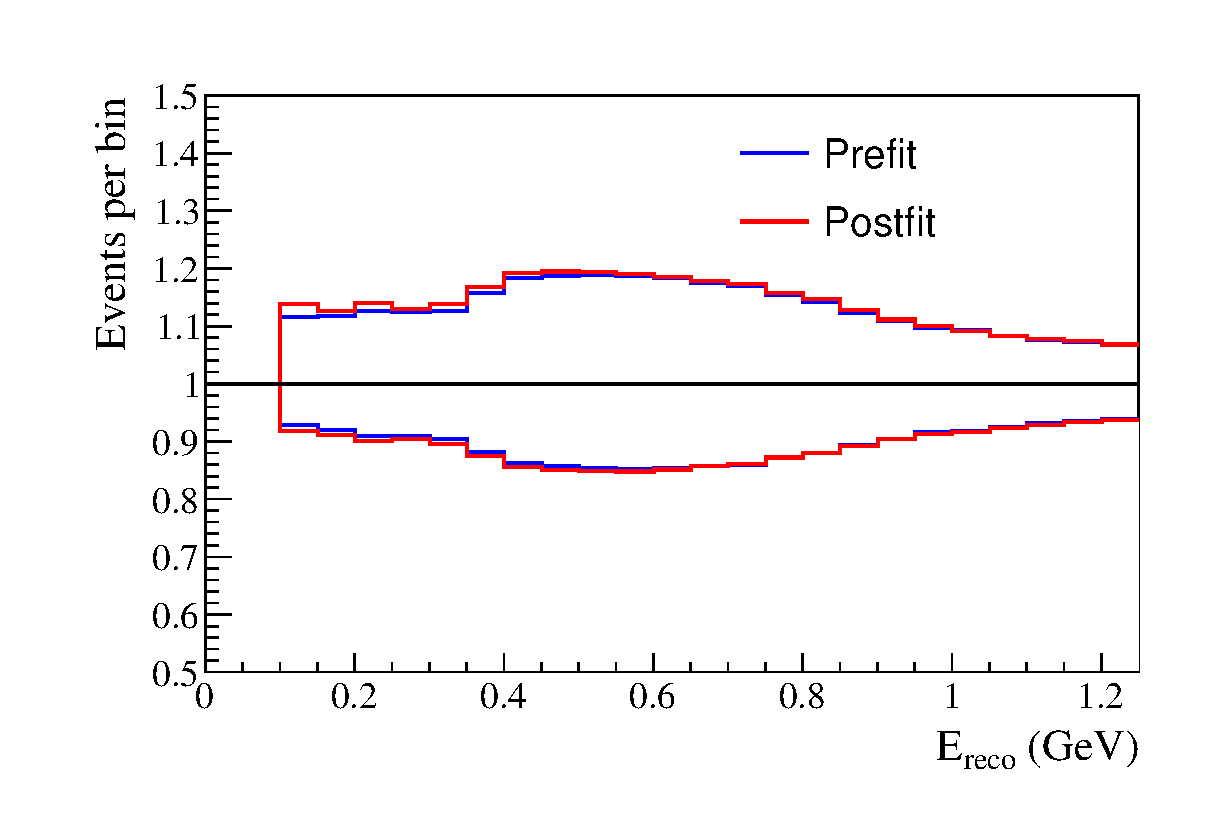
\includegraphics[width=18pc]{./nuebar_plots/spectrum_tweaked/oscillated_Osc_param_envelope_ratio.eps}
%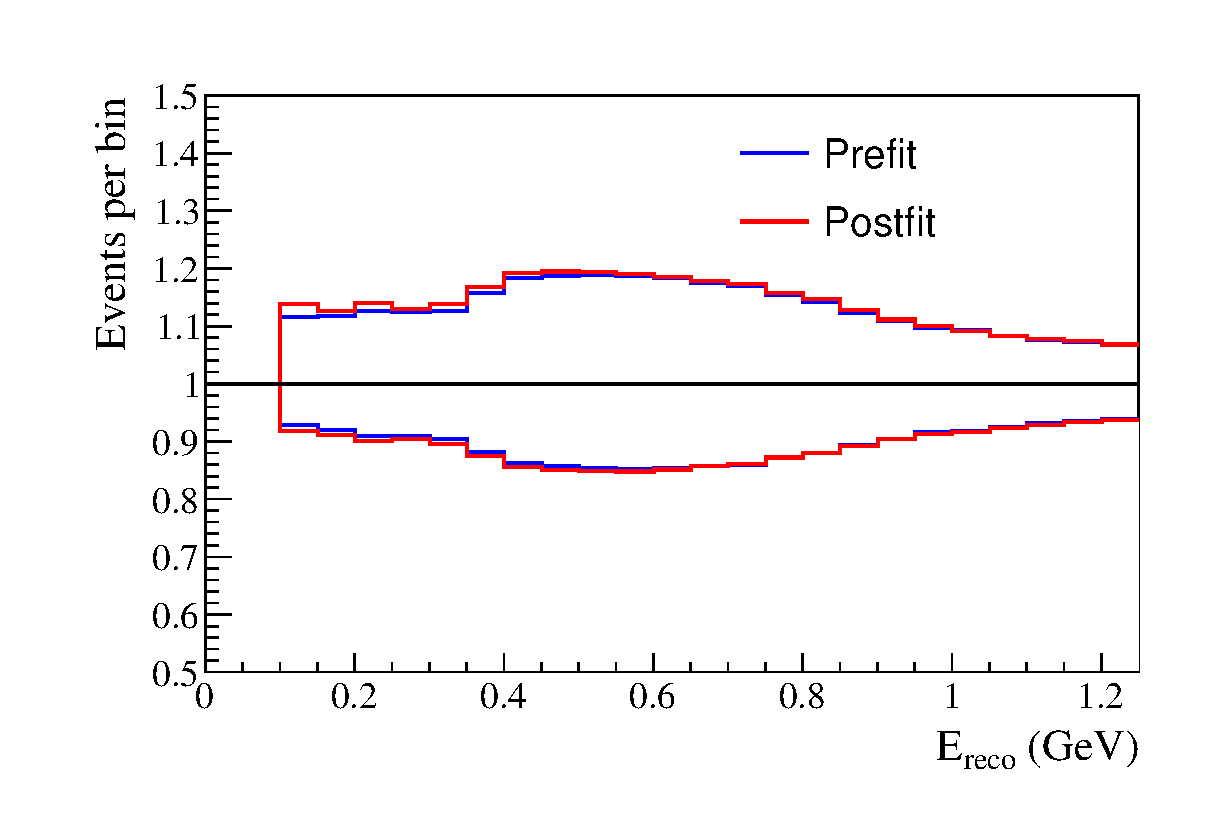
\includegraphics[width=18pc]{./nuebar_plots/spectrum_tweaked/oscillated_Osc_param_envelope_ratio.eps}
%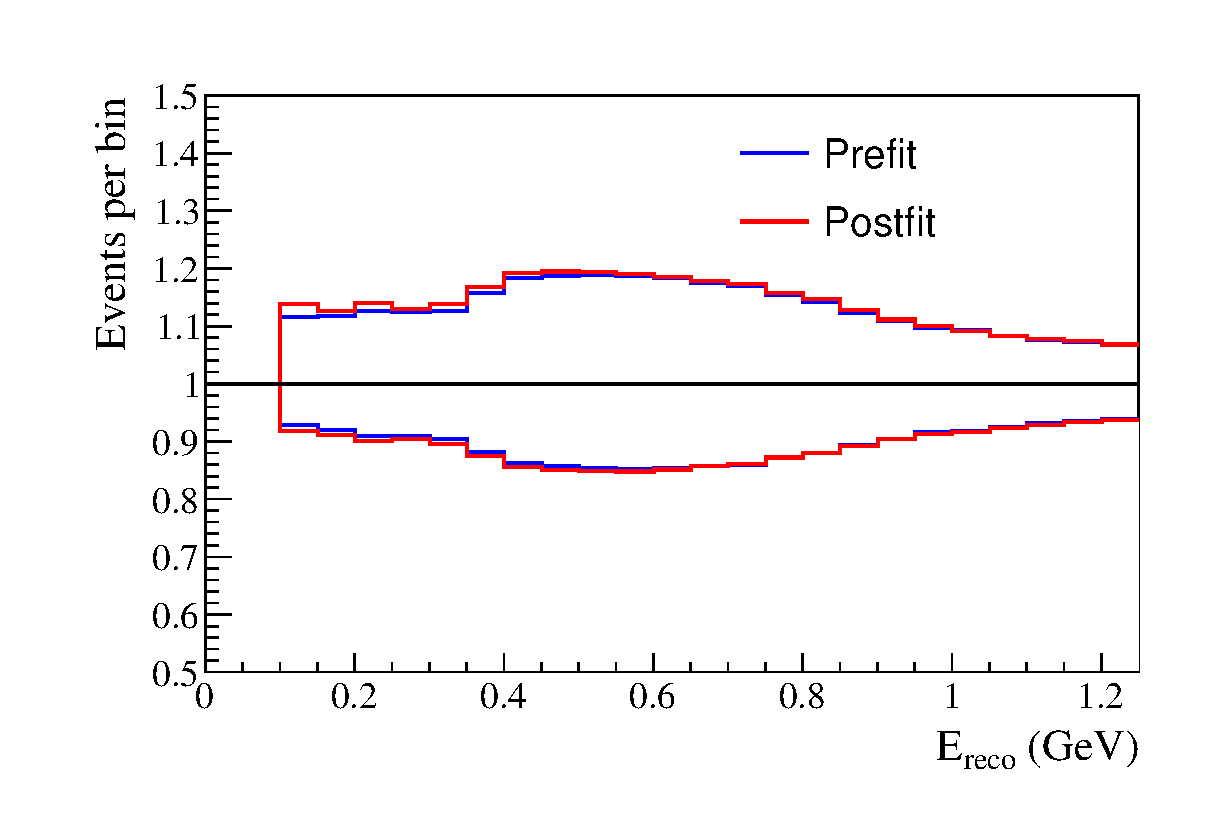
\includegraphics[width=18pc]{./nuebar_plots/spectrum_tweaked/oscillated_Osc_param_envelope_ratio.eps}
%%
\includegraphics[width=20pc]{./images/missing_plot-eps-converted-to.pdf}
%\caption {
%    \huge{TO UPDATE} % caption is already ok
%%  Error envelopes, expressed as a ratio of event count, for the energy spectrum as a result of oscillation parameters
%%    for an exposure 
%%  of \TotalPotNu POT in neutrino mode
%%  and
%%  of \TotalPotNuBar POT in antineutrino mode.
%%  From top left to bottom right the following samples are shown:
%%  $\mu$-like neutrino mode,
%%  $\mu$-like antineutrino mode,
%%  $e$-like neutrino mode
%%  and 
%%  $e$-like antineutrino mode.
%%  \NumToys toy MC experiments were generated with randomized systematic parameters and the 1$\sigma$ spread of bin contents was calculated.
%%  BANFF tuned MC templates were used.
%%  All systematic parameters were considered and their correlations were taken into account.
%%  The fractional error in each bin corresponds to the $1\sigma$ error 
%%  obtained from the distribution of the extracted number of events.
%%  First the median is found. 
%%  Then the upper (lower) error corresponds
%%  to the number of events for which the 34\% of toys is contained
%%  in the right (left) side of the median.
%%  The continuos line shows the pre-BANFF (blue) and post-BANFF (red) ratios.
%%   The oscillation parameters shown in Tab.~\ref{tab:osc_params_joint} are used.
%}
%\label{fig:Osc_envelope_ratio}
%\end{figure*}
%
%
%\begin{figure*}[htb]
%\center
%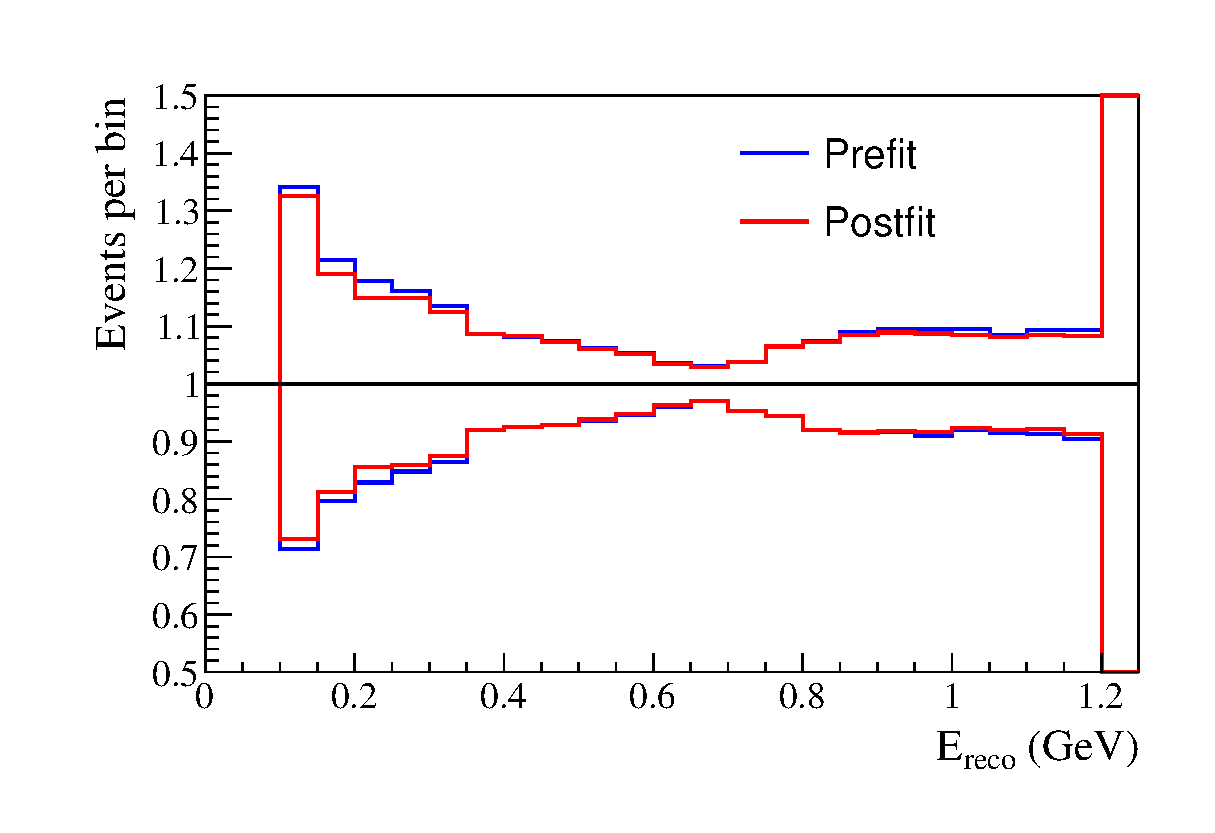
\includegraphics[width=18pc]{./nuebar_plots/spectrum_tweaked/oscillated_SKDet_FSI_envelope_ratio.eps}
%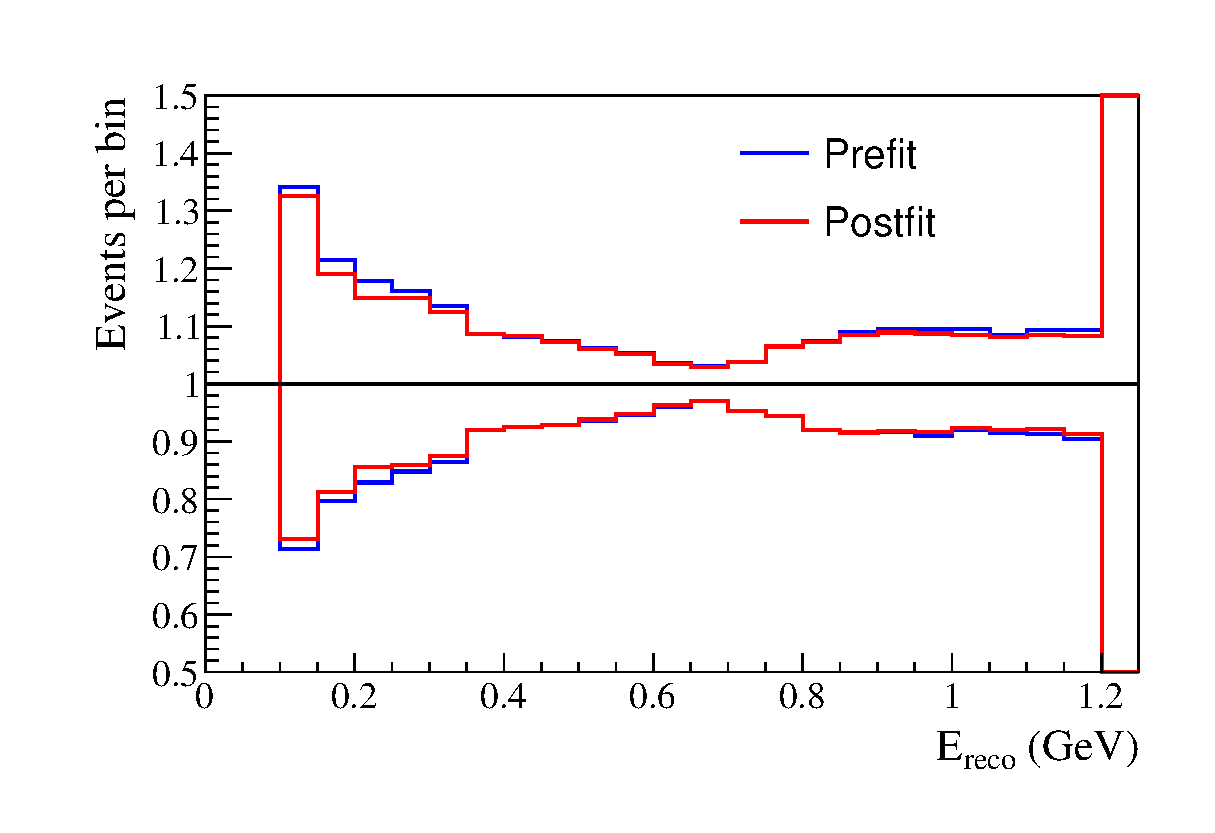
\includegraphics[width=18pc]{./nuebar_plots/spectrum_tweaked/oscillated_SKDet_FSI_envelope_ratio.eps}
%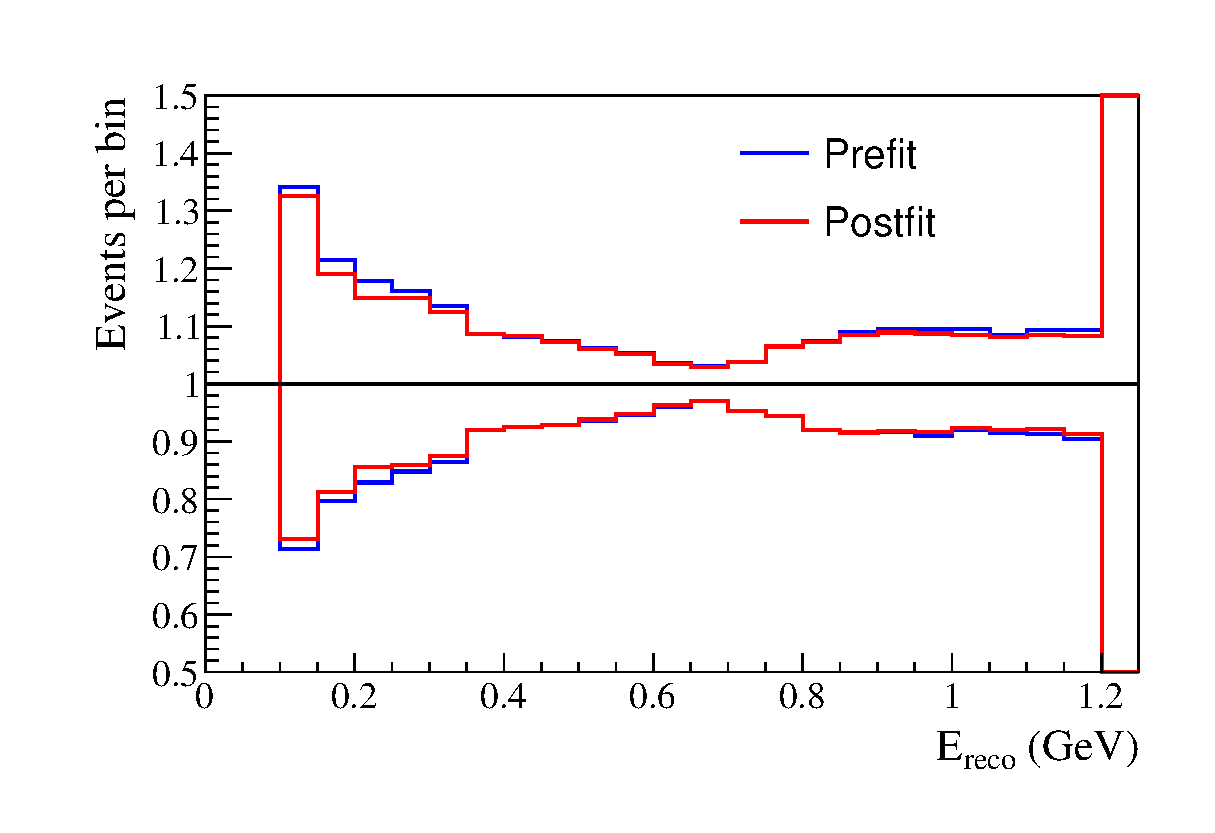
\includegraphics[width=18pc]{./nuebar_plots/spectrum_tweaked/oscillated_SKDet_FSI_envelope_ratio.eps}
%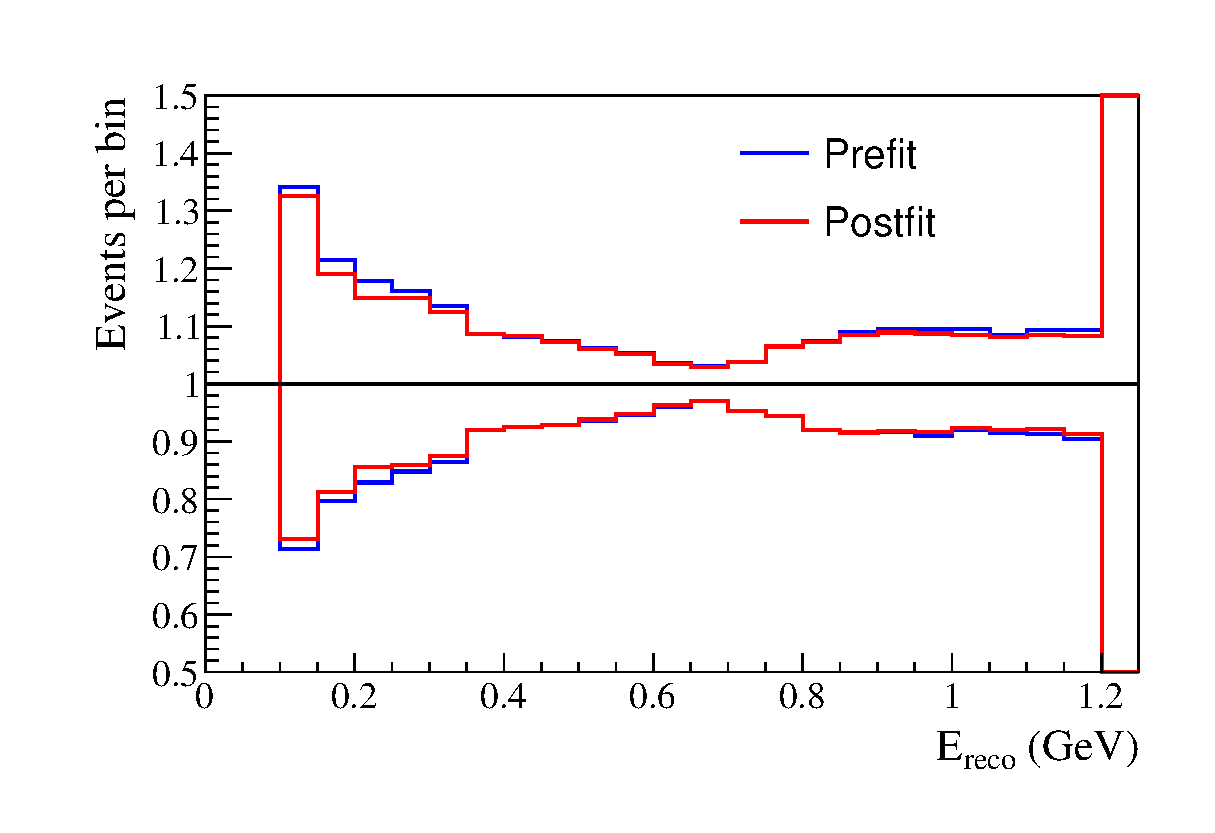
\includegraphics[width=18pc]{./nuebar_plots/spectrum_tweaked/oscillated_SKDet_FSI_envelope_ratio.eps}
%%
\includegraphics[width=20pc]{./images/missing_plot-eps-converted-to.pdf}
%\caption {
%    \huge{TO UPDATE} % caption is already ok
%%  Error envelopes, expressed as a ratio of event count, for the energy spectrum as a result of Super-K detector and FSI/SI parameters
%%    for an exposure 
%%  of \TotalPotNu POT in neutrino mode
%%  and
%%  of \TotalPotNuBar POT in antineutrino mode.
%%  From top left to bottom right the following samples are shown:
%%  $\mu$-like neutrino mode,
%%  $\mu$-like antineutrino mode,
%%  $e$-like neutrino mode
%%  and 
%%  $e$-like antineutrino mode.
%%  \NumToys toy MC experiments were generated with randomized systematic parameters and the 1$\sigma$ spread of bin contents was calculated.
%%  BANFF tuned MC templates were used.
%%  All systematic parameters were considered and their correlations were taken into account.
%%  The fractional error in each bin corresponds to the $1\sigma$ error 
%%  obtained from the distribution of the extracted number of events.
%%  First the median (red line) is found. 
%%  Then the upper (lower) error corresponds
%%  to the number of events for which the 34\% of toys is contained
%%  in the right (left) side of the median.
%%  The continuos line shows the pre-BANFF (blue) and post-BANFF (red) ratios.
%%     The oscillation parameters shown in Tab.~\ref{tab:osc_params_joint} are used.
%}
%\label{fig:SKDet_FSI_envelope_ratio}
%\end{figure*}
%
%\begin{figure*}[htb]
%\center
%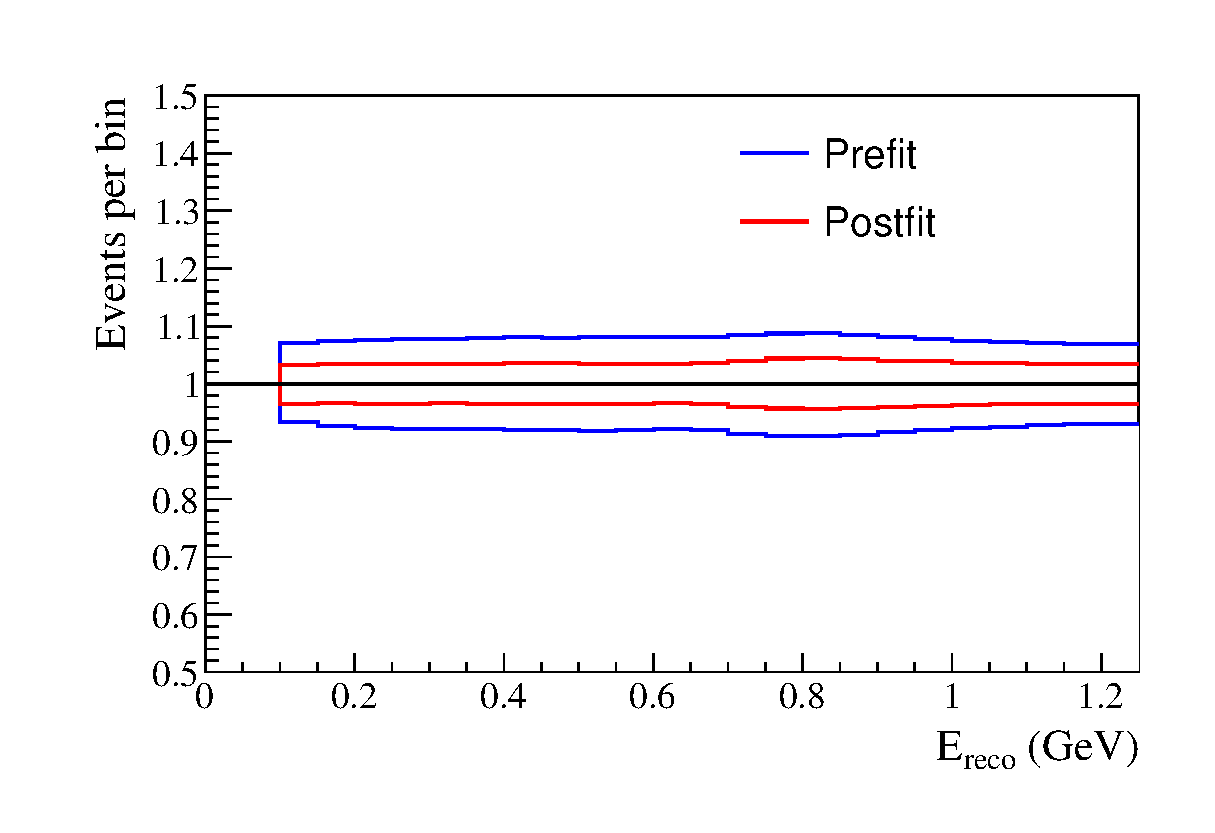
\includegraphics[width=18pc]{./nuebar_plots/spectrum_tweaked/oscillated_BANFF_flux_envelope_ratio.eps}
%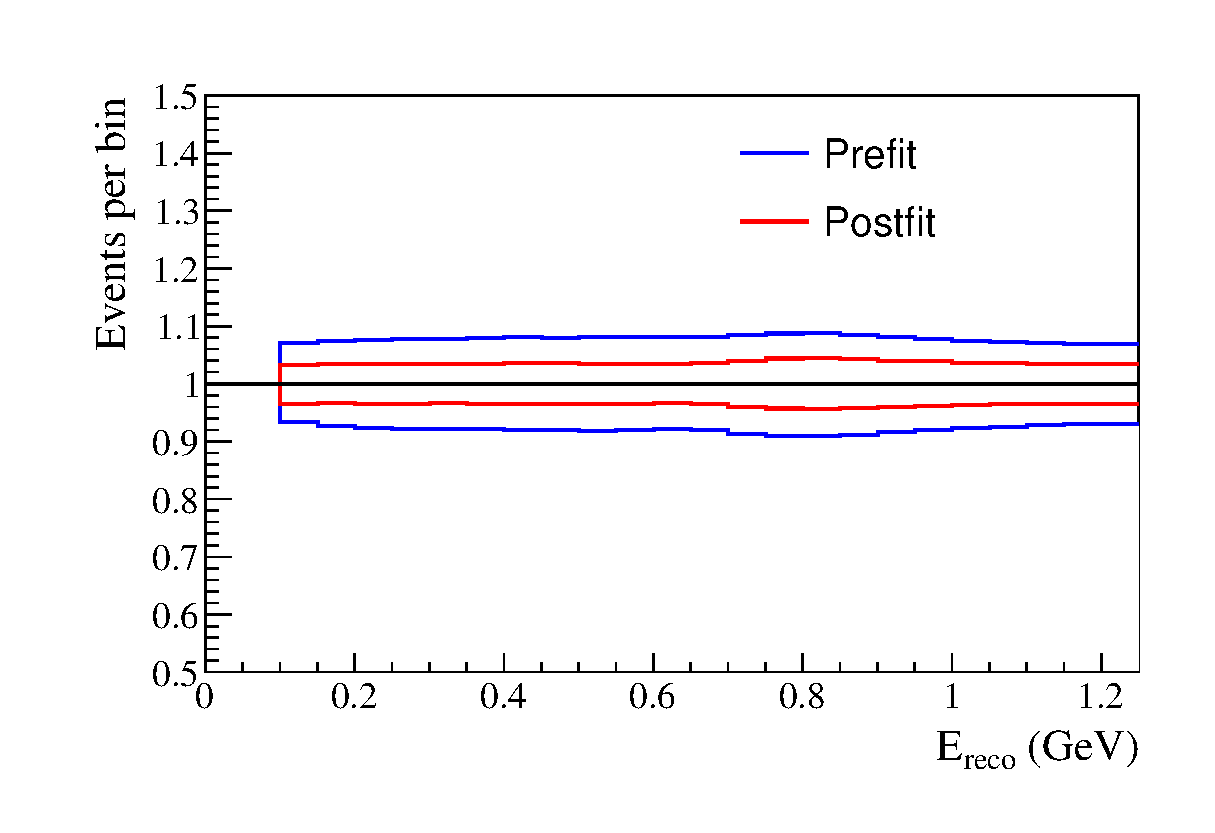
\includegraphics[width=18pc]{./nuebar_plots/spectrum_tweaked/oscillated_BANFF_flux_envelope_ratio.eps}
%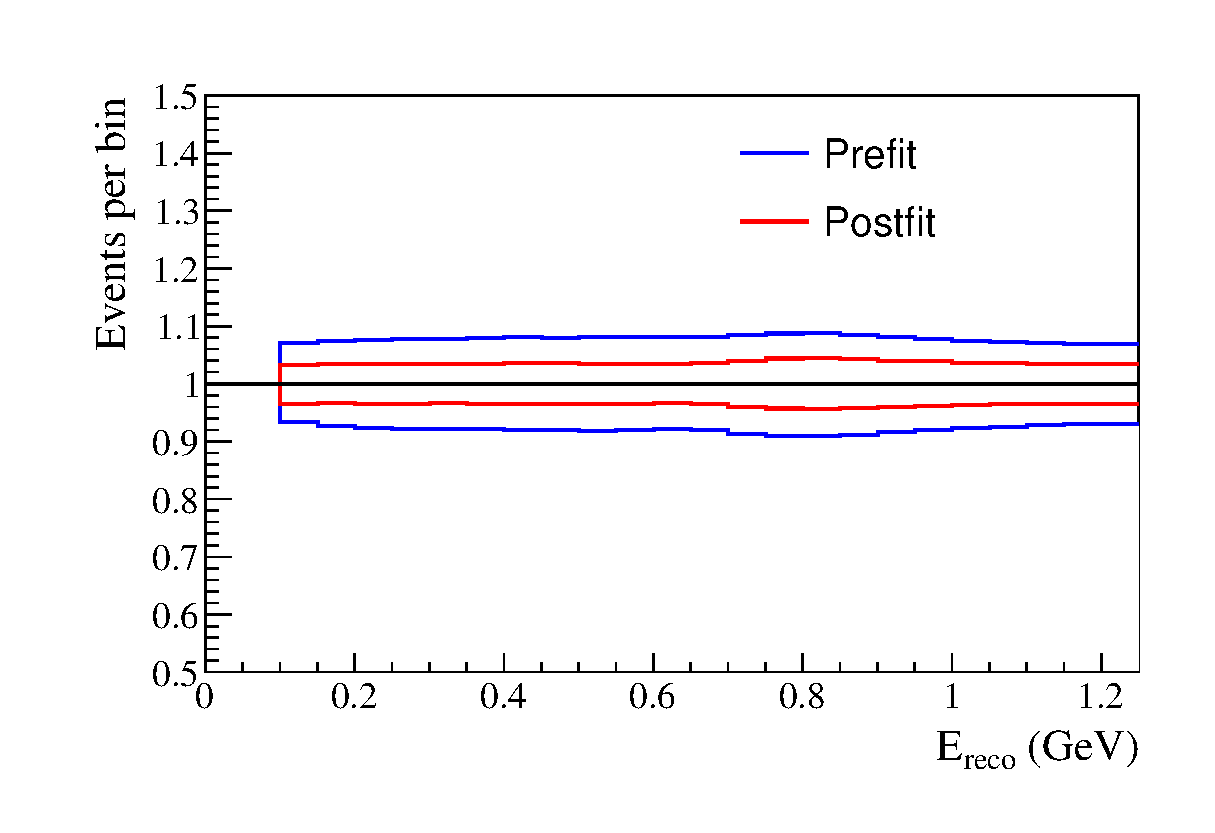
\includegraphics[width=18pc]{./nuebar_plots/spectrum_tweaked/oscillated_BANFF_flux_envelope_ratio.eps}
%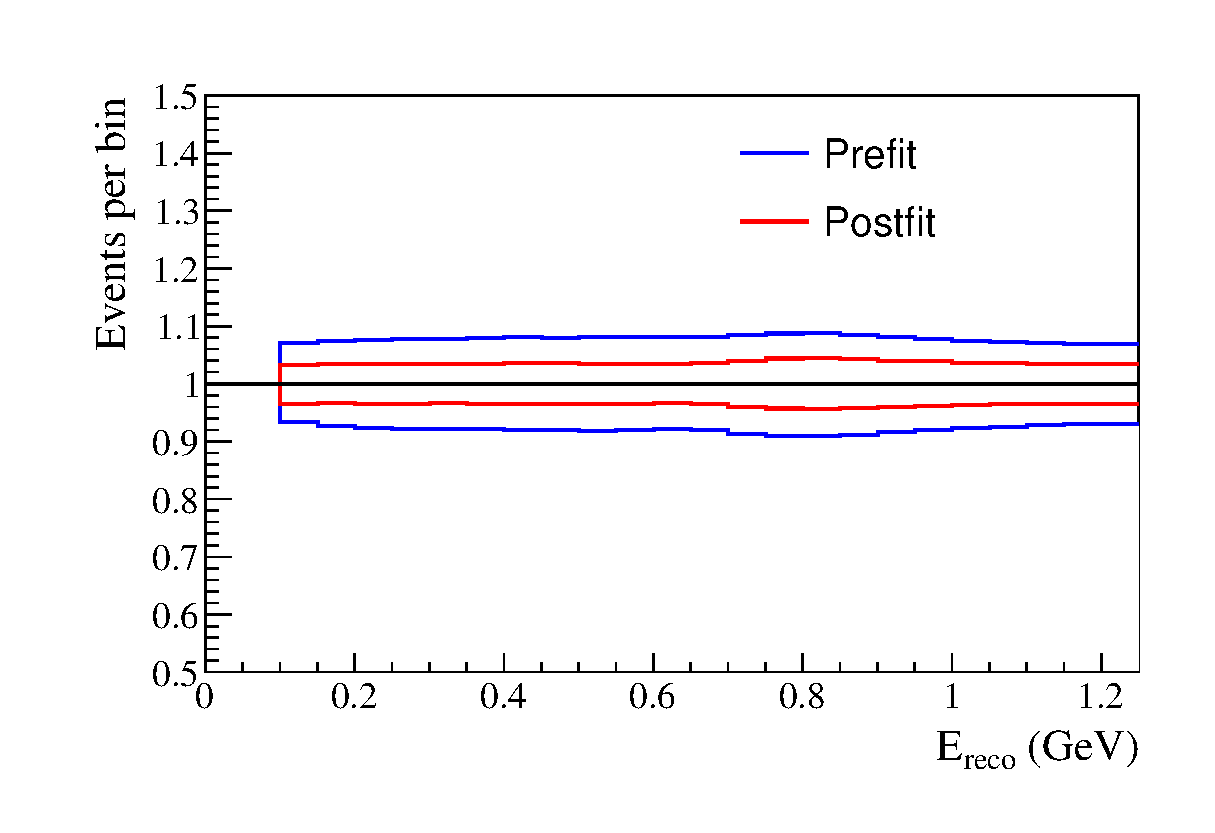
\includegraphics[width=18pc]{./nuebar_plots/spectrum_tweaked/oscillated_BANFF_flux_envelope_ratio.eps}
%%
\includegraphics[width=20pc]{./images/missing_plot-eps-converted-to.pdf}
%\caption {
%    \huge{TO UPDATE} % caption is already ok
%%  Error envelopes, expressed as a ratio of event count, for the energy spectrum as a result of flux systematics
%%    for an exposure 
%%  of \TotalPotNu POT in neutrino mode
%%  and
%%  of \TotalPotNuBar POT in antineutrino mode.
%%  From top left to bottom right the following samples are shown:
%%  $\mu$-like neutrino mode,
%%  $\mu$-like antineutrino mode,
%%  $e$-like neutrino mode
%%  and 
%%  $e$-like antineutrino mode.
%%  \NumToys toy MC experiments were generated with randomized systematic parameters and the 1$\sigma$ spread of bin contents was calculated.
%%  BANFF tuned MC templates were used.
%%  All systematic parameters were considered and their correlations were taken into account.
%%  The fractional error in each bin corresponds to the $1\sigma$ error 
%%  obtained from the distribution of the extracted number of events.
%%  First the median (red line) is found. 
%%  Then the upper (lower) error corresponds
%%  to the number of events for which the 34\% of toys is contained
%%  in the right (left) side of the median.
%%  The continuos line shows the pre-BANFF (blue) and post-BANFF (red) ratios.
%%   The oscillation parameters shown in Tab.~\ref{tab:osc_params_joint} are used.
%}
%\label{fig:flux_envelope_ratio}
%\end{figure*}
%
%
%\begin{figure*}[htb]
%\center
%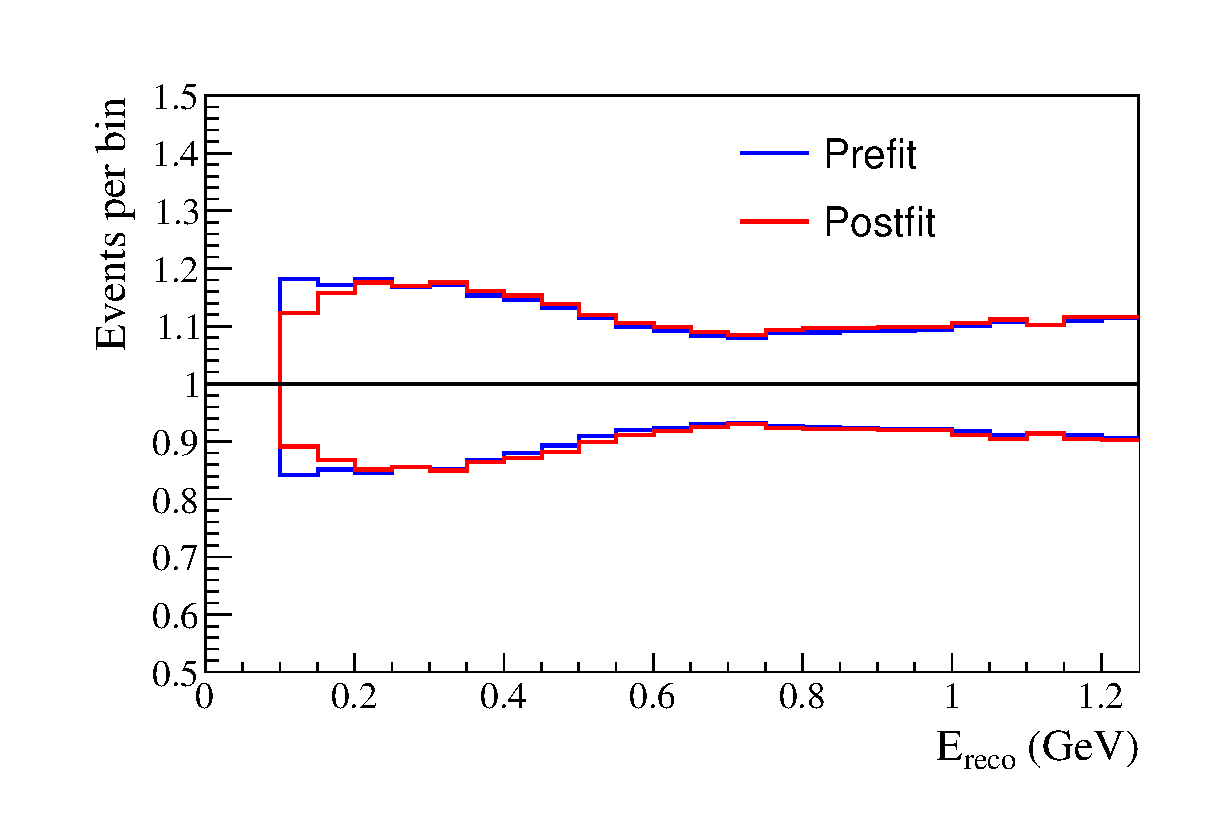
\includegraphics[width=18pc]{./nuebar_plots/spectrum_tweaked/oscillated_BANFF_xsec_envelope_ratio.eps}
%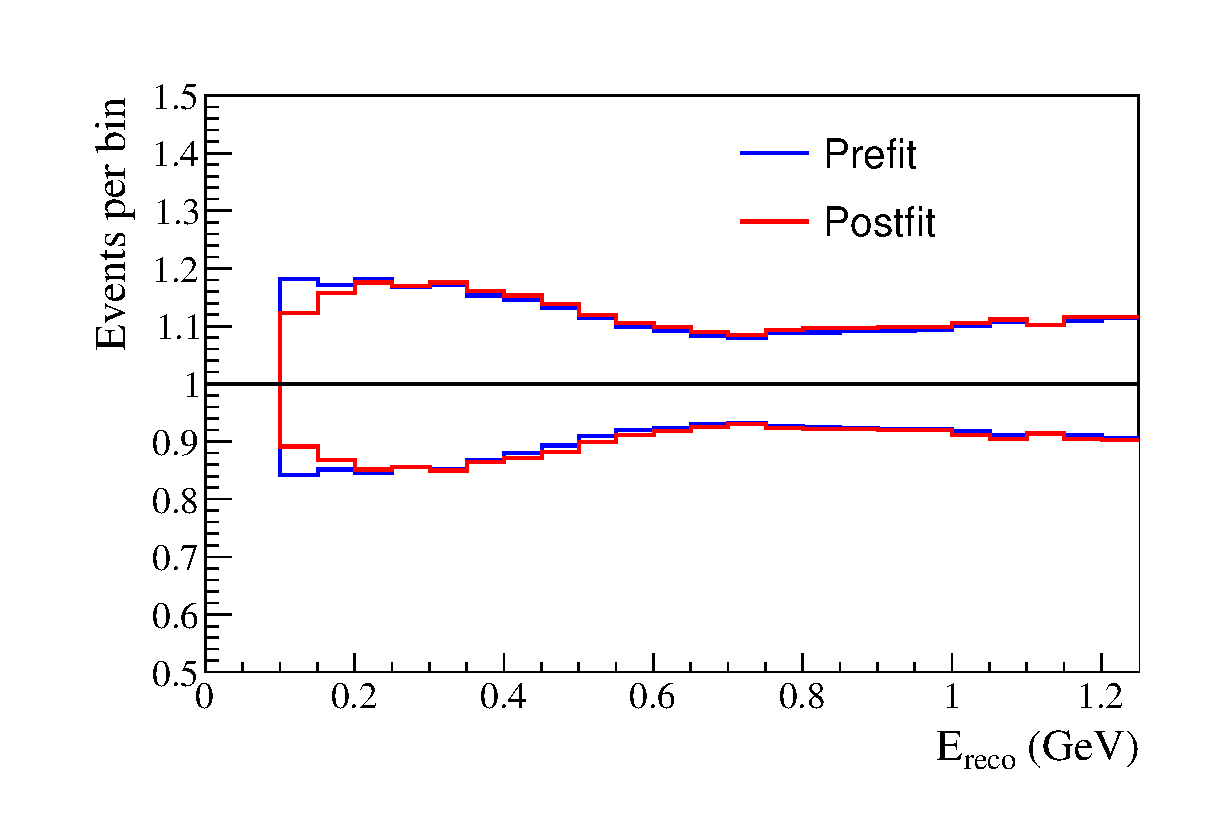
\includegraphics[width=18pc]{./nuebar_plots/spectrum_tweaked/oscillated_BANFF_xsec_envelope_ratio.eps}
%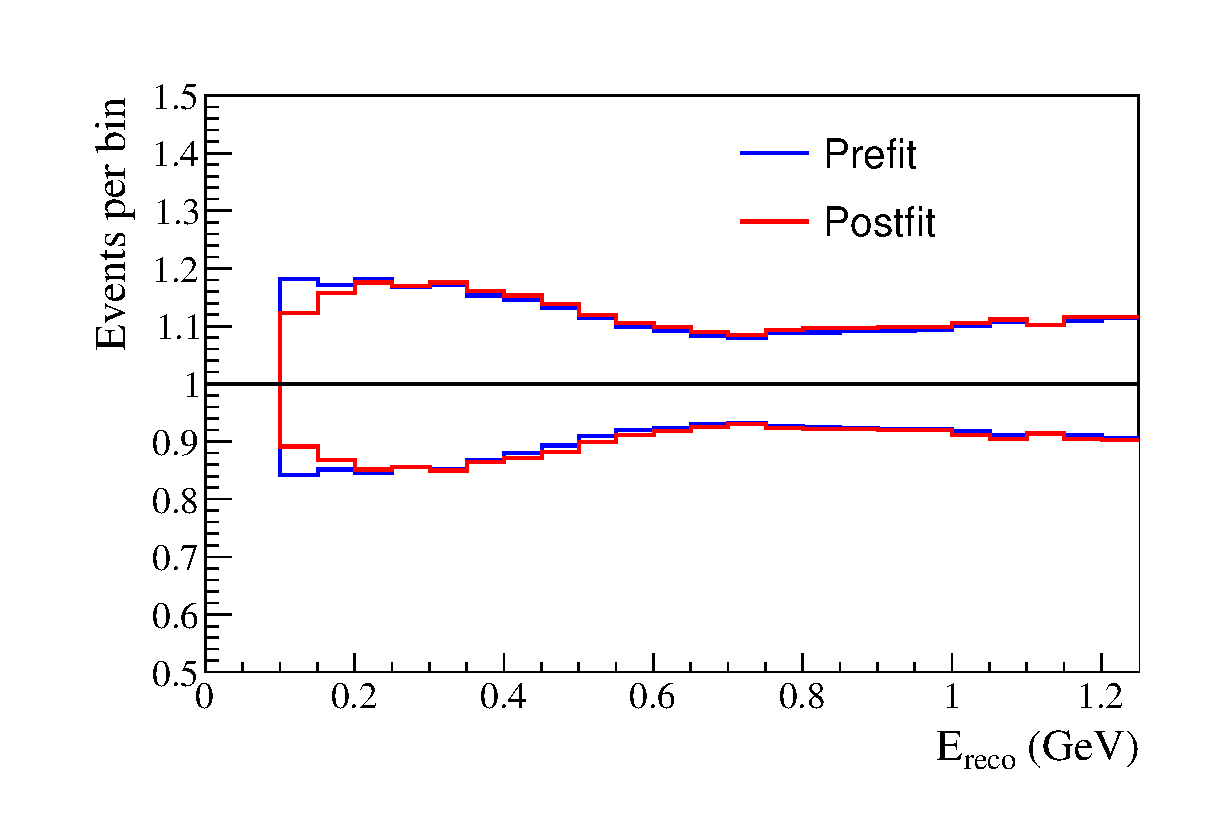
\includegraphics[width=18pc]{./nuebar_plots/spectrum_tweaked/oscillated_BANFF_xsec_envelope_ratio.eps}
%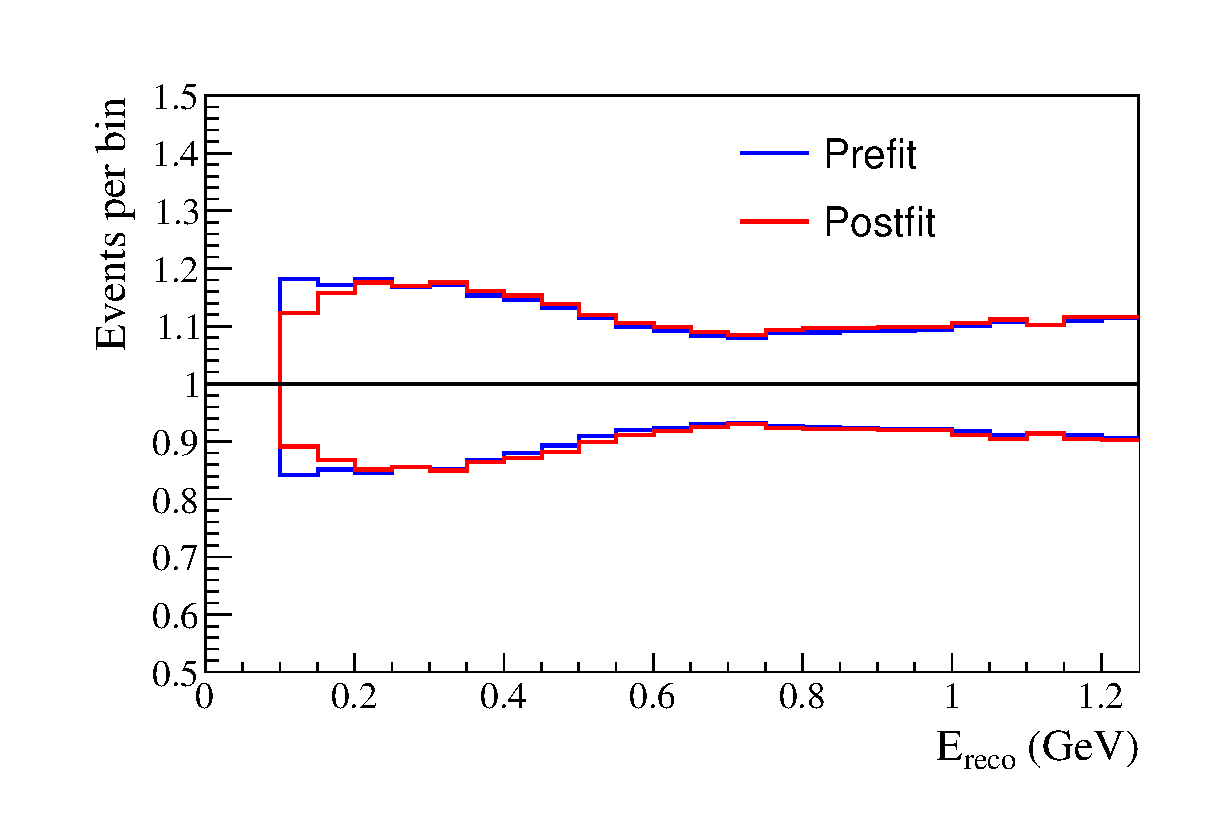
\includegraphics[width=18pc]{./nuebar_plots/spectrum_tweaked/oscillated_BANFF_xsec_envelope_ratio.eps}
%%
\includegraphics[width=20pc]{./images/missing_plot-eps-converted-to.pdf}
%\caption {
%    \huge{TO UPDATE} % caption is already ok
%%  Error envelopes, expressed as a ratio of event count, for the energy spectrum as a result of only cross-section parameters
%%    for an exposure 
%%  of \TotalPotNu POT in neutrino mode
%%  and
%%  of \TotalPotNuBar POT in antineutrino mode.
%%  From top left to bottom right the following samples are shown:
%%  $\mu$-like neutrino mode,
%%  $\mu$-like antineutrino mode,
%%  $e$-like neutrino mode
%%  and 
%%  $e$-like antineutrino mode.
%%  \NumToys toy MC experiments were generated with randomized systematic parameters and the 1$\sigma$ spread of bin contents was calculated.
%%  BANFF tuned MC templates were used.
%%  All systematic parameters were considered and their correlations were taken into account.
%%  The fractional error in each bin corresponds to the $1\sigma$ error 
%%  obtained from the distribution of the extracted number of events.
%%  First the median (red line) is found. 
%%  Then the upper (lower) error corresponds
%%  to the number of events for which the 34\% of toys is contained
%%  in the right (left) side of the median.
%%  The continuos line shows the pre-BANFF (blue) and post-BANFF (red) ratios.
%%     The oscillation parameters shown in Tab.~\ref{tab:osc_params_joint} are used.
%}
%\label{fig:xsec_envelope_ratio}
%\end{figure*}
%
%\begin{figure*}[htb]
%\center
%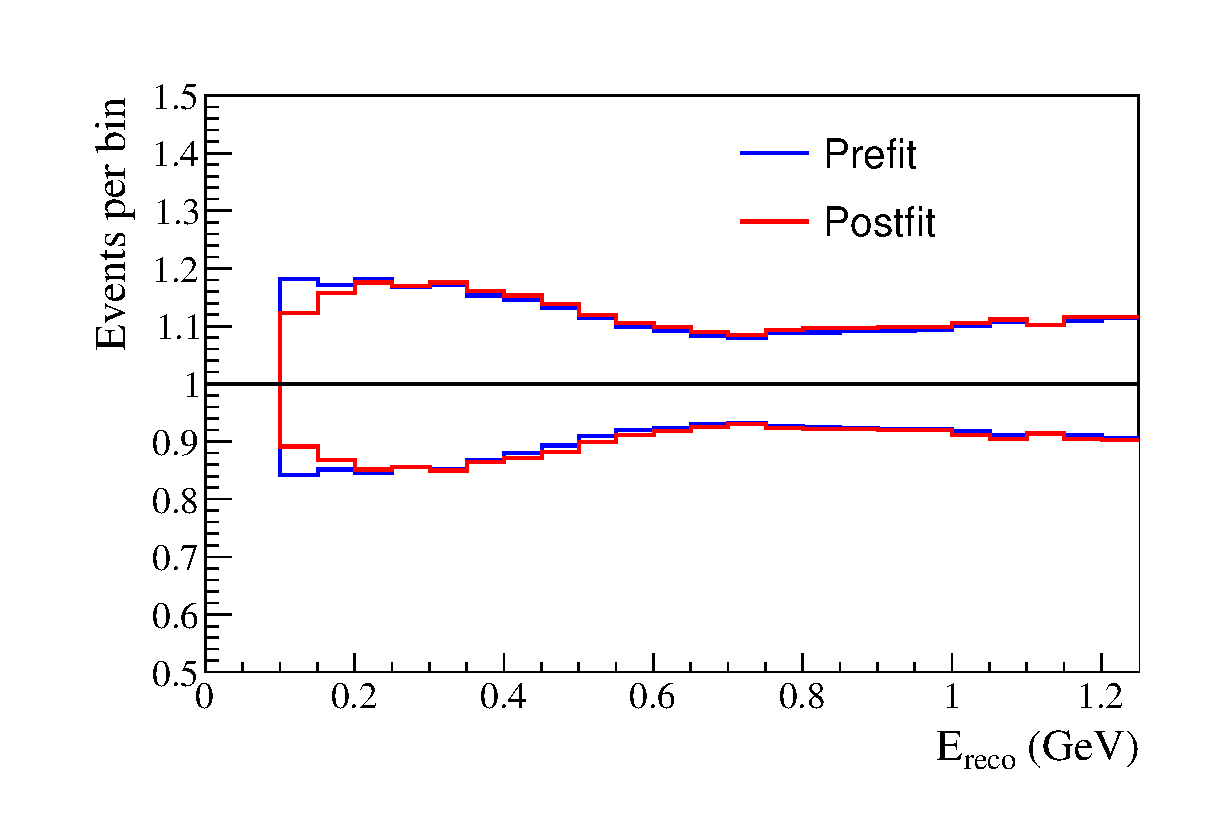
\includegraphics[width=18pc]{./nuebar_plots/spectrum_tweaked/oscillated_BANFF_xsec_envelope_ratio.eps}
%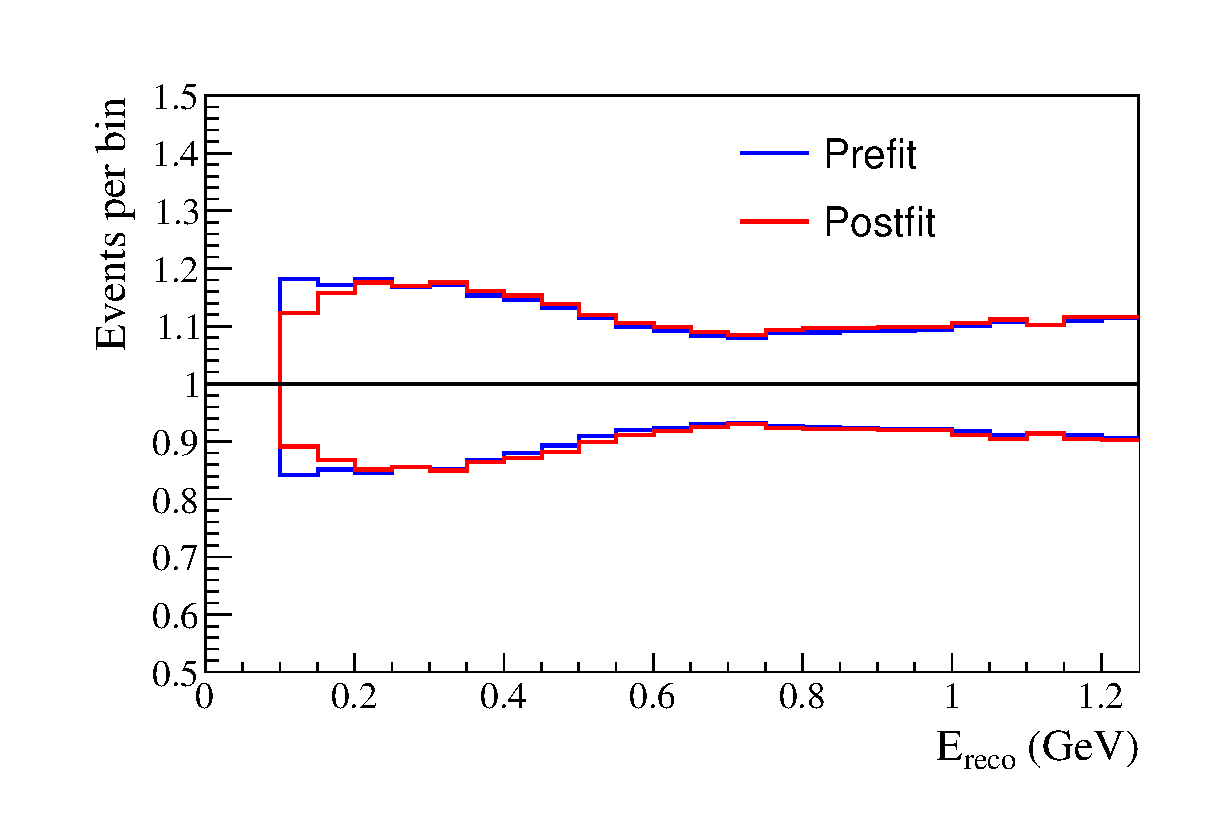
\includegraphics[width=18pc]{./nuebar_plots/spectrum_tweaked/oscillated_BANFF_xsec_envelope_ratio.eps}
%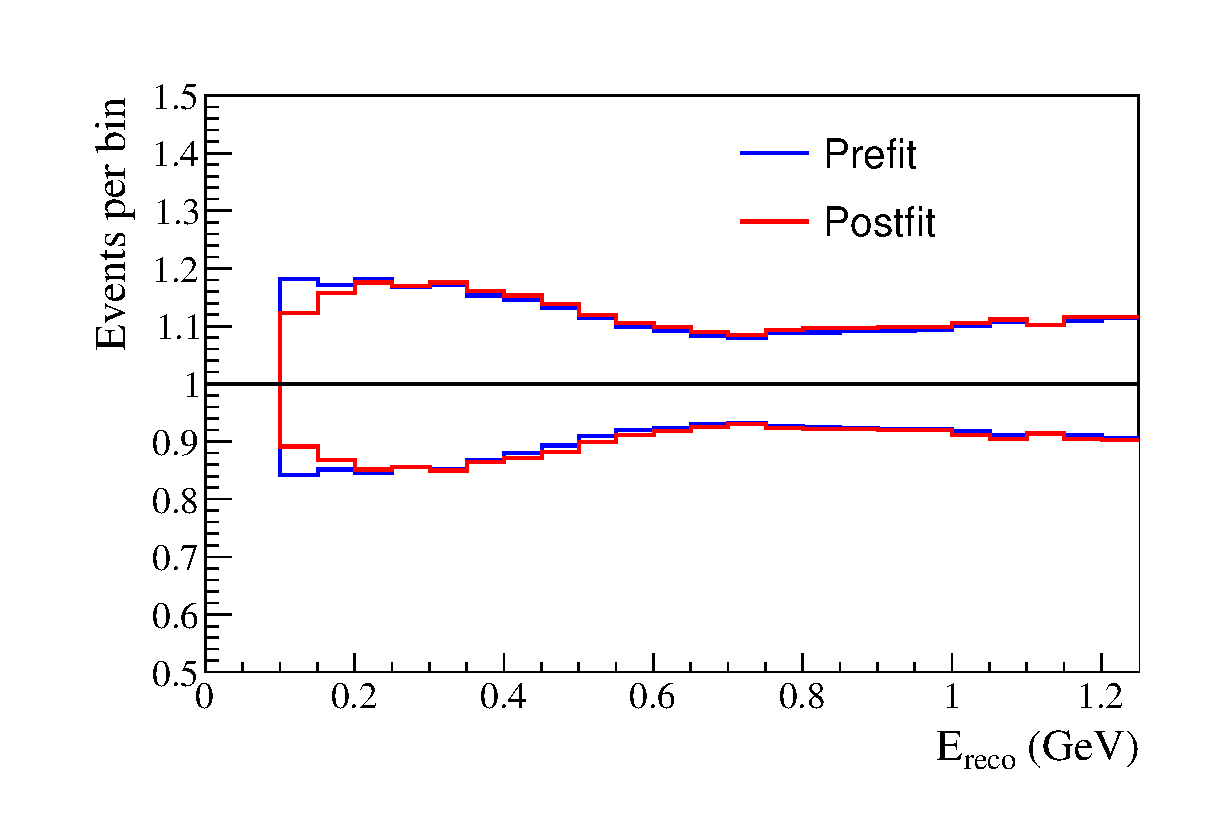
\includegraphics[width=18pc]{./nuebar_plots/spectrum_tweaked/oscillated_BANFF_xsec_envelope_ratio.eps}
%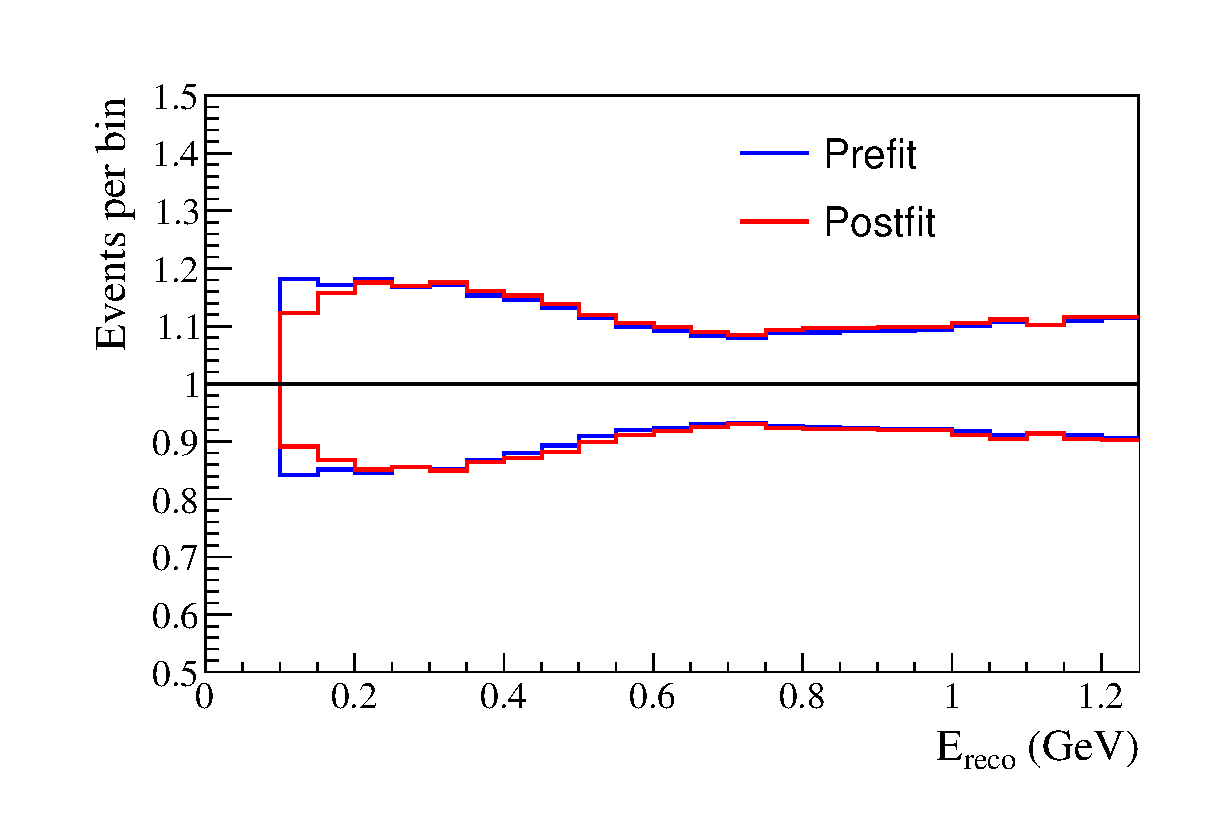
\includegraphics[width=18pc]{./nuebar_plots/spectrum_tweaked/oscillated_BANFF_xsec_envelope_ratio.eps}
%%
\includegraphics[width=20pc]{./images/missing_plot-eps-converted-to.pdf}
%\caption {
%    \huge{TO UPDATE} % caption is already ok
%%  Error envelopes, expressed as a ratio of event count, for the energy spectrum as a result of flux and cross-section parameters
%%    for an exposure 
%%  of \TotalPotNu POT in neutrino mode
%%  and
%%  of \TotalPotNuBar POT in antineutrino mode.
%%  From top left to bottom right the following samples are shown:
%%  $\mu$-like neutrino mode,
%%  $\mu$-like antineutrino mode,
%%  $e$-like neutrino mode
%%  and 
%%  $e$-like antineutrino mode.
%%  \NumToys toy MC experiments were generated with randomized systematic parameters and the 1$\sigma$ spread of bin contents was calculated.
%%  BANFF tuned MC templates were used.
%%  All systematic parameters were considered and their correlations were taken into account.
%%  The fractional error in each bin corresponds to the $1\sigma$ error 
%%  obtained from the distribution of the extracted number of events.
%%  First the median (red line) is found. 
%%  Then the upper (lower) error corresponds
%%  to the number of events for which the 34\% of toys is contained
%%  in the right (left) side of the median.
%%  The continuos line shows the pre-BANFF (blue) and post-BANFF (red) ratios.
%%     The oscillation parameters shown in Tab.~\ref{tab:osc_params_joint} are used.
%}
%\label{fig:flux_xsec_envelope_ratio}
%\end{figure*}
%
%\begin{figure*}[htb]
%\center
%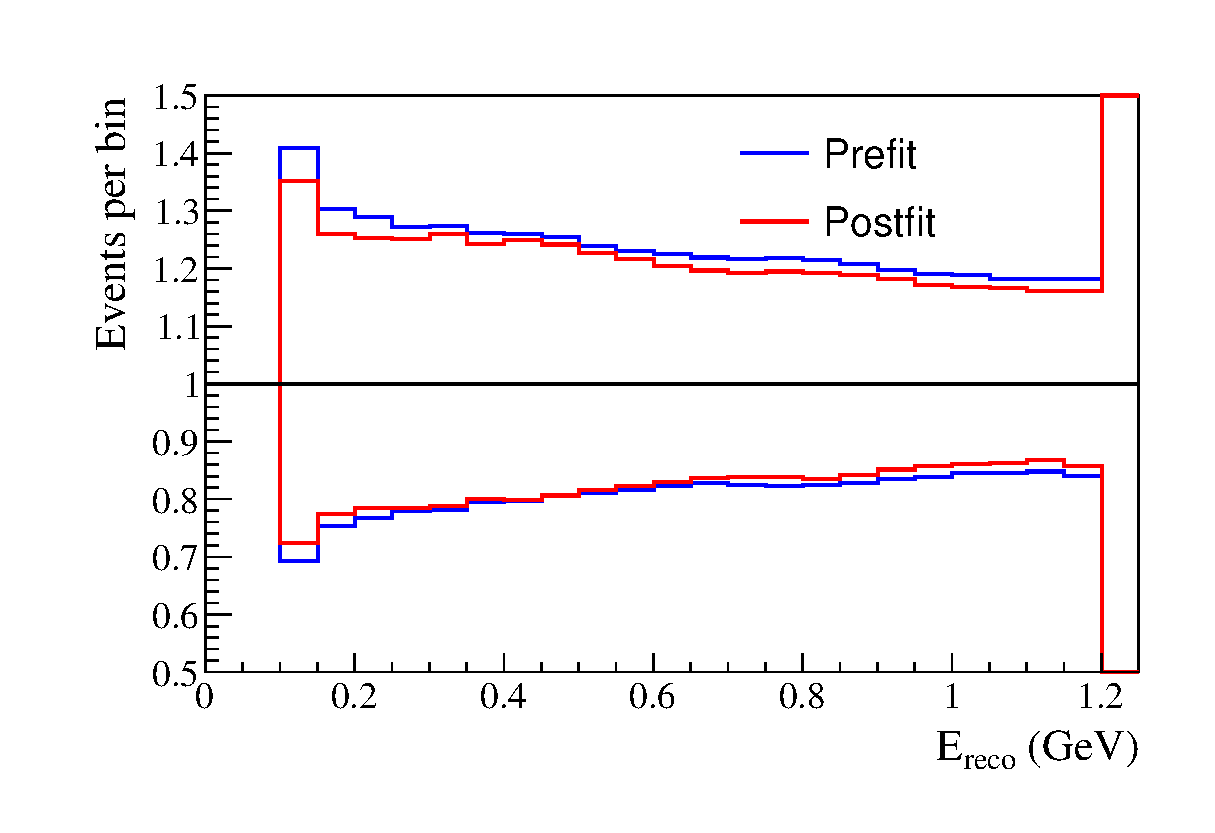
\includegraphics[width=18pc]{./nuebar_plots/spectrum_tweaked/oscillated_all_envelope_ratio.eps}
%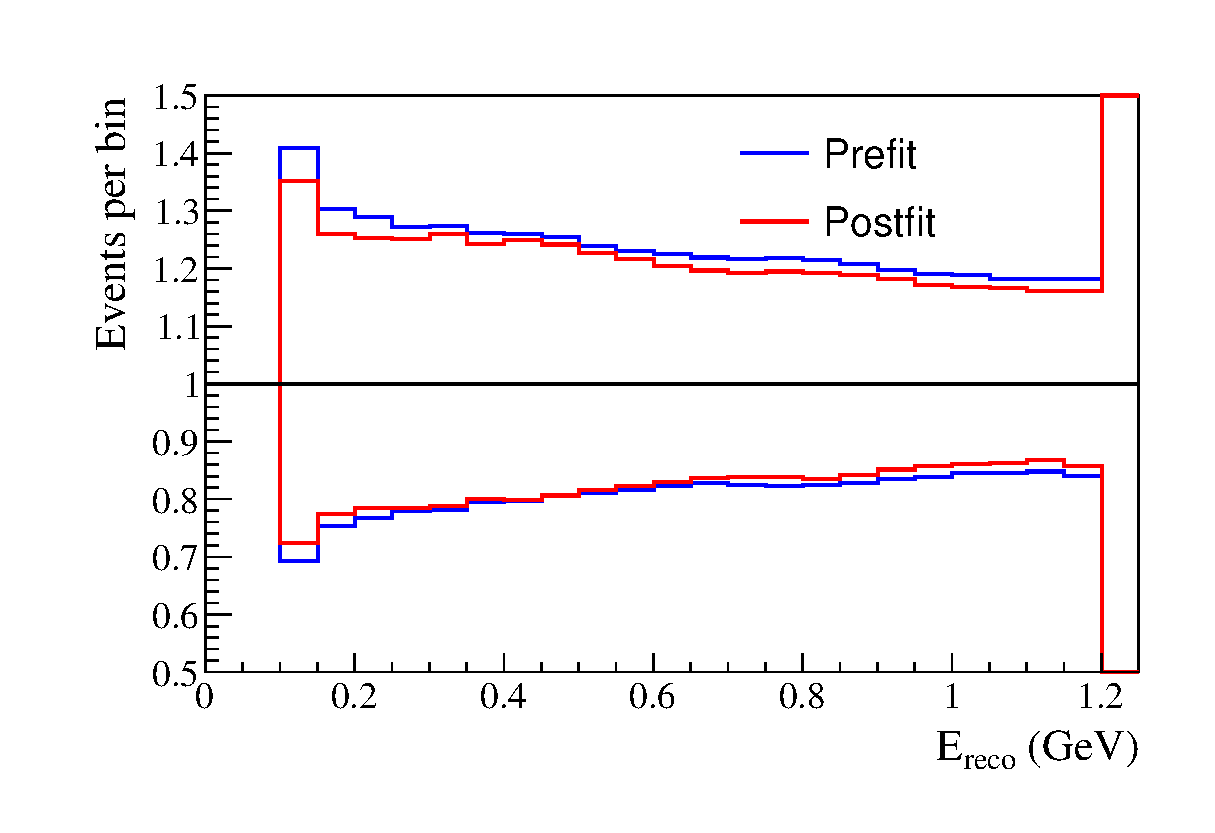
\includegraphics[width=18pc]{./nuebar_plots/spectrum_tweaked/oscillated_all_envelope_ratio.eps}
%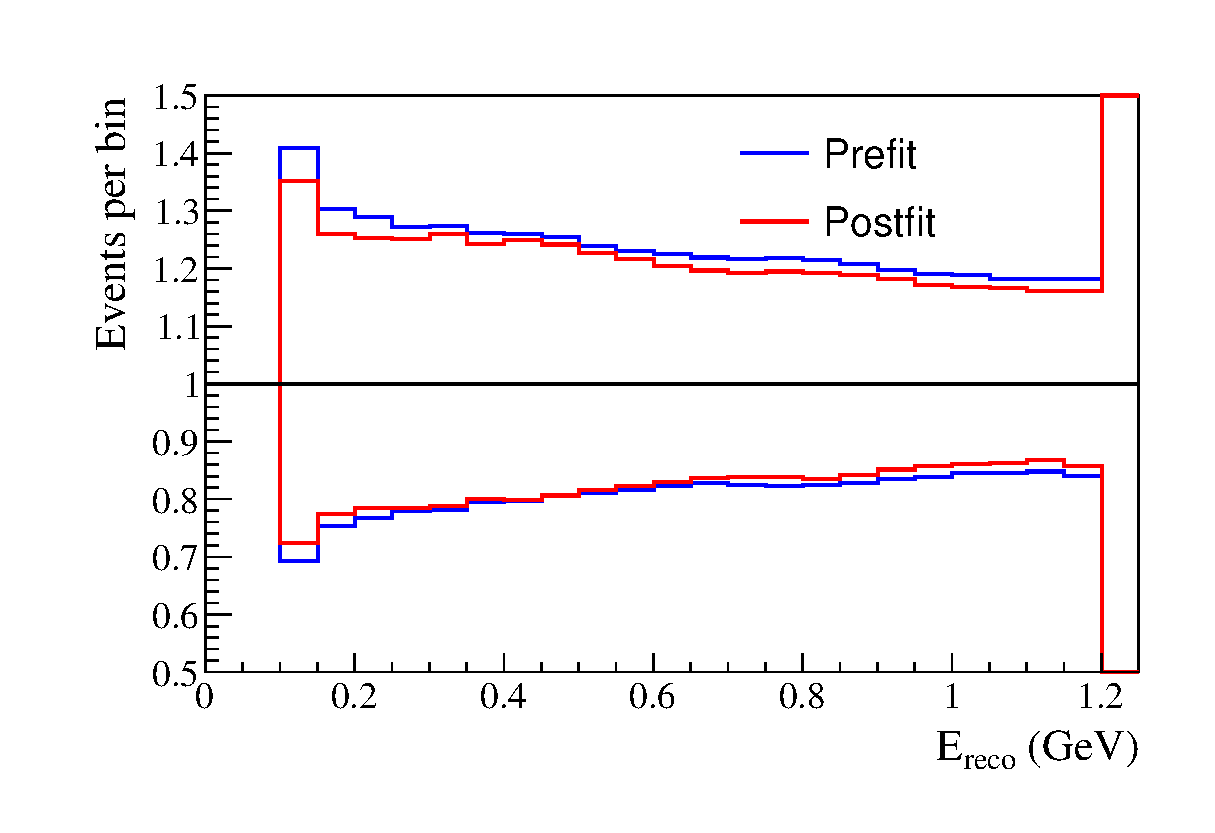
\includegraphics[width=18pc]{./nuebar_plots/spectrum_tweaked/oscillated_all_envelope_ratio.eps}
%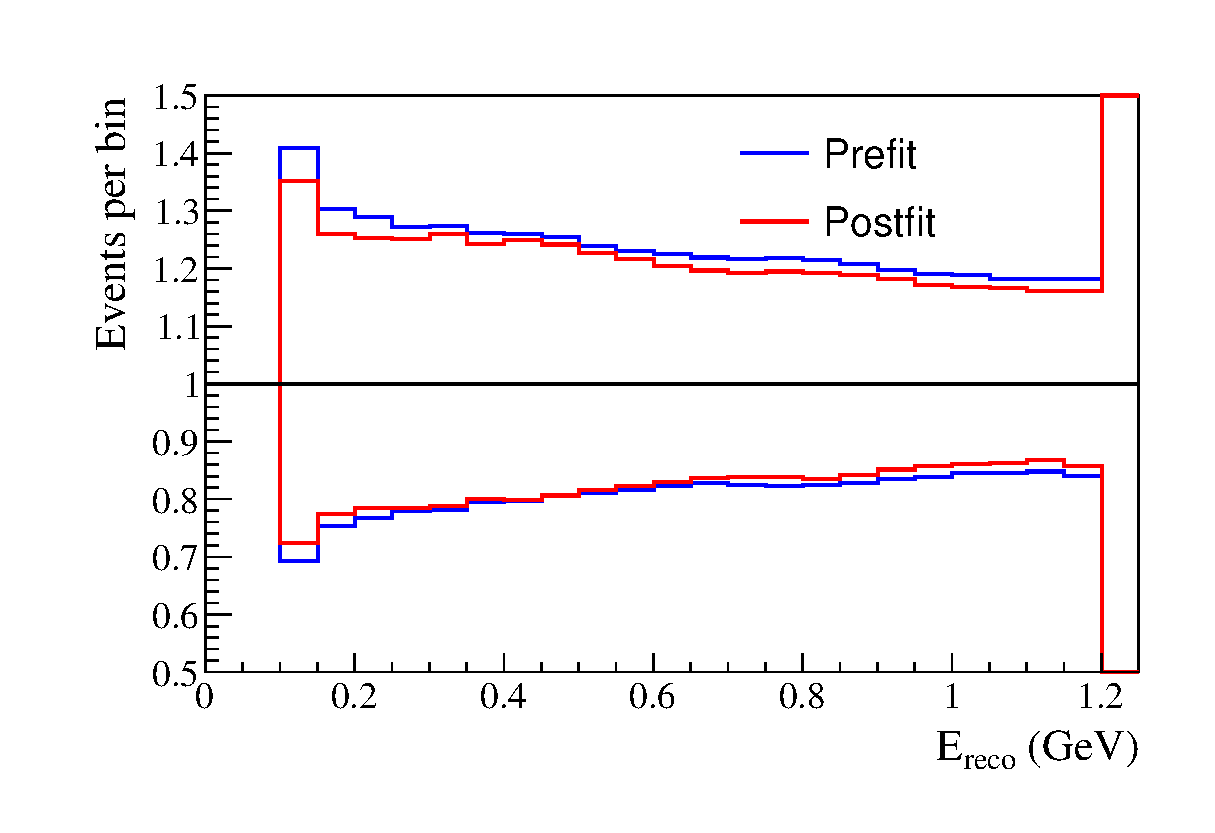
\includegraphics[width=18pc]{./nuebar_plots/spectrum_tweaked/oscillated_all_envelope_ratio.eps}
%%
\includegraphics[width=20pc]{./images/missing_plot-eps-converted-to.pdf}
%\caption {
%    \huge{TO UPDATE} % caption is already ok
%%  Error envelopes, expressed as a ratio of event count, for the energy spectrum as a result of all systematic parameters
%%    for an exposure 
%%  of \TotalPotNu POT in neutrino mode
%%  and
%%  of \TotalPotNuBar POT in antineutrino mode.
%%  From top left to bottom right the following samples are shown:
%%  $\mu$-like neutrino mode,
%%  $\mu$-like antineutrino mode,
%%  $e$-like neutrino mode
%%  and 
%%  $e$-like antineutrino mode.
%%  \NumToys toy MC experiments were generated with randomized systematic parameters and the 1$\sigma$ spread of bin contents was calculated.
%%  BANFF tuned MC templates were used.
%%  All systematic parameters were considered and their correlations were taken into account.
%%  The fractional error in each bin corresponds to the $1\sigma$ error 
%%  obtained from the distribution of the extracted number of events.
%%  First the median (red line) is found. 
%%  Then the upper (lower) error corresponds
%%  to the number of events for which the 34\% of toys is contained
%%  in the right (left) side of the median.
%%  The continuos line shows the pre-BANFF (blue) and post-BANFF (red) ratios.
%%   The oscillation parameters shown in Tab.~\ref{tab:osc_params_joint} are used.
%}
%\label{fig:all_envelope_ratio}
%\end{figure*}
%
%
%\clearpage
%
%







% Asimov A w/o flux bias

In tab.~\ref{tab:nsk_systematic_table_summary_joint_asimov_A_fhc_mulike_NoFluxBias},
\ref{tab:nsk_systematic_table_summary_joint_asimov_A_fhc_elike_NoFluxBias},
\ref{tab:nsk_systematic_table_summary_joint_asimov_A_rhc_mulike_NoFluxBias}
and
\ref{tab:nsk_systematic_table_summary_joint_asimov_A_rhc_elike_NoFluxBias}
%\ref{tab:ratio_systematic_table_summary_asimov_B}
the effect of each group of systematic uncertainties 
on the total number of events and on the ratio 
between neutrino and antineutrino mode is shown for the Asimov data set A,
but without taking into account the correction of the post-fit BANFF systematic
parameters as well the additional covariance matrix that take into account
the bias in the flux parameters of the BANFF fit.
The impact of the uncertainty due to the bias of the BANFF fit is small
and has a small impact compared to the other systematic uncertainties.


%%% fhc mu-like

\begin{table}[htb]
\centering
\begin{tabular}{| c | c | c |}
\hline
  {\bf Source of uncertainty}    & \multicolumn{1}{c|}{{\bf ${\delta}N_{SK}$/$N_{SK}$}}\\
                                 & \multicolumn{1}{c|}{(Asimov A)}\\

\hline
\hline  SKDet+FSI+SI                   & 4.11\%                        \\
\hline
\hline
  Flux                           & 3.26\%                        \\
\hline
\hline
  2p-2h (corr)                     & 3.53\%                        \\
  2p-2h-bar (corr)                  & 0.20\%                        \\
  NC other (uncorr)              & 0.79\%                        \\
  NC 1gamma (uncorr)             & 0.00\%                        \\
  XSec nue/numu (uncorr)                 & 0.01\%                        \\
\hline
  XSec Tot (corr)                  & 3.96\%                        \\
  XSec Tot                       & 4.04\%                        \\
\hline
\hline
  Flux+XSec                      & 2.75\%                        \\
\hline
\hline
  Flux+XSec+SKDet+FSI+SI         & 5.03\%                        \\
\hline
\hline
  Oscillations                   & 0.03\%                        \\
\hline
\hline
  All                            & 5.00\%                        \\
\hline
\hline

\end{tabular}
\caption{
 Effect of 1$\sigma$ variations of the groups of systematics parameters on total number of
 1-ring muon-like events for neutrino mode obtained by performing 10k toys MC.
The systematic parameter values measured with the ND280 data 
shown in 
\cref{tab:banff_uncertainties_flux_fhc},
~\ref{tab:banff_uncertainties_flux_rhc}
~\ref{tab:banff_uncertainties_xsec}
and
~\ref{tab:banff_uncertainties_skdetfsi}
and the oscillation parameters of the Asimov data set A shown in \cref{tab:osc_params_joint_asimov}
are used.
Since the parameters $\theta_{23}$ and $\Delta m^2_{32}$ ($\Delta m^2_{13}$)
will be measured,
only the uncertainty on the parameters 
$\sin^2 \theta_{13}$,
$\sin^2 \theta_{12}$
and 
$\Delta m^2_{21}$ 
are taken into account.
The correction of the post-fit BANFF parameters as well as the additional covariance matrix 
used to take account for bias in the BANFF fit is not applied.
}                                                                                                                                                                                          
\label{tab:nsk_systematic_table_summary_joint_asimov_A_fhc_mulike_NoFluxBias}
\end{table}




%%%%% fhc e-like


\begin{table}[htb]
\centering
\begin{tabular}{| c | c | c |}
\hline
  {\bf Source of uncertainty}    & \multicolumn{1}{c|}{{\bf ${\delta}N_{SK}$/$N_{SK}$}}\\
                                 & \multicolumn{1}{c|}{(Asimov A)}\\

\hline
\hline  SKDet+FSI+SI                   & 3.47\%                        \\
\hline
  Flux                           & 3.40\%                        \\
\hline
\hline
  2p-2h (corr)                     & 3.95\%                        \\
  2p-2h-bar (corr)                  & 0.05\%                        \\
  NC other (uncorr)              & 0.16\%                        \\
  NC 1gamma (uncorr)             & 1.49\%                        \\
  XSec nue/numu (uncorr)                 & 2.63\%                        \\
\hline
  XSec Tot (corr)                  & 4.17\%                        \\
  XSec Tot                       & 5.15\%                        \\
\hline
\hline
  Flux+XSec                      & 4.08\%                        \\
\hline
  Flux+XSec+SKDet+FSI+SI         & 5.51\%                        \\
\hline
\hline
  Oscillations                   & 4.19\%                        \\
\hline
\hline
  All                            & 6.93\%                        \\
\hline
\hline

\end{tabular}
\caption{
 Effect of 1$\sigma$ variations of the groups of systematics parameters on total number of
 1-ring electron-like events for neutrino mode obtained by performing 10k toys MC.
The systematic parameter values measured with the ND280 data 
shown in 
\cref{tab:banff_uncertainties_flux_fhc},
~\ref{tab:banff_uncertainties_flux_rhc}
~\ref{tab:banff_uncertainties_xsec}
and
~\ref{tab:banff_uncertainties_skdetfsi}
and the oscillation parameters of the Asimov data set A shown in \cref{tab:osc_params_joint_asimov}
are used.
Since the parameters $\theta_{23}$ and $\Delta m^2_{32}$ ($\Delta m^2_{13}$)
will be measured,
only the uncertainty on the parameters 
$\sin^2 \theta_{13}$,
$\sin^2 \theta_{12}$
and 
$\Delta m^2_{21}$ 
are taken into account.
The correction of the post-fit BANFF parameters as well as the additional covariance matrix 
used to take account for bias in the BANFF fit is not applied.
}                                                                                                                                                                                          
\label{tab:nsk_systematic_table_summary_joint_asimov_A_fhc_elike_NoFluxBias}
\end{table}



%%%%%% rhc mu-like


\begin{table}[htb]
\centering
\begin{tabular}{| c | c | c |}
\hline
  {\bf Source of uncertainty}    & \multicolumn{1}{c|}{{\bf ${\delta}N_{SK}$/$N_{SK}$}}\\
                                 & \multicolumn{1}{c|}{(Asimov A)}\\

\hline
\hline  SKDet+FSI+SI                   & 3.94\%                        \\
\hline
\hline
  Flux                           & 3.40\%                        \\
\hline
\hline
  2p-2h (corr)                     & 3.00\%                        \\
  2p-2h-bar (corr)                  & 1.76\%                        \\
  NC other (uncorr)              & 0.76\%                        \\
  NC 1gamma (uncorr)             & 0.00\%                        \\
  XSec nue/numu (uncorr)                 & 0.00\%                        \\
\hline  
  XSec Tot (corr)                  & 4.20\%                        \\
  XSec Tot                       & 4.27\%                        \\
\hline
\hline
  Flux+XSec                      & 2.90\%                        \\
\hline
\hline
  Flux+XSec+SKDet+FSI+SI         & 4.90\%                        \\
\hline
\hline
  Oscillations                   & 0.03\%                        \\
\hline
\hline
  All                            & 4.91\%                        \\
\hline
\hline

\end{tabular}

\caption{
 Effect of 1$\sigma$ variations of the groups of systematics parameters on total number of
 1-ring muon-like events for antineutrino mode obtained by performing 10k toys MC.
The systematic parameter values measured with the ND280 data 
shown in 
\cref{tab:banff_uncertainties_flux_fhc},
~\ref{tab:banff_uncertainties_flux_rhc}
~\ref{tab:banff_uncertainties_xsec}
and
~\ref{tab:banff_uncertainties_skdetfsi}
and the oscillation parameters of the Asimov data set A shown in \cref{tab:osc_params_joint_asimov}
are used.
Since the parameters $\theta_{23}$ and $\Delta m^2_{32}$ ($\Delta m^2_{13}$)
will be measured,
only the uncertainty on the parameters 
$\sin^2 \theta_{13}$,
$\sin^2 \theta_{12}$
and 
$\Delta m^2_{21}$ 
are taken into account.
The correction of the post-fit BANFF parameters as well as the additional covariance matrix 
used to take account for bias in the BANFF fit is not applied.
}                                                                                                                                                                                          
\label{tab:nsk_systematic_table_summary_joint_asimov_A_rhc_mulike_NoFluxBias}
\end{table}



%%%%%% rhc e-like

\begin{table}[htb]
\centering
\begin{tabular}{| c | c | c |}
\hline
  {\bf Source of uncertainty}    & \multicolumn{1}{c|}{{\bf ${\delta}N_{SK}$/$N_{SK}$}}\\
                                 & \multicolumn{1}{c|}{(Asimov A)}\\

\hline
\hline  SKDet+FSI+SI                   & 3.94\%                        \\
\hline
\hline
  Flux                           & 3.53\%                        \\
\hline
\hline
  2p-2h (corr)                     & 3.11\%                        \\
  2p-2h-bar (corr)                  & 2.24\%                        \\
  NC other (uncorr)              & 0.33\%                        \\
  NC 1gamma (uncorr)             & 2.98\%                        \\
  XSec nue/numu (uncorr)                 & 1.52\%                        \\
\hline  
  XSec Tot (corr)                  & 4.44\%                        \\
  XSec Tot                       & 5.57\%                        \\
\hline
\hline
  Flux+XSec                      & 4.39\%                        \\
\hline
\hline
  Flux+XSec+SKDet+FSI+SI         & 6.11\%                        \\
\hline
\hline
  Oscillations                   & 3.98\%                        \\
\hline
\hline
  All                            & 7.24\%                        \\
\hline
\hline

\end{tabular}
\caption{
 Effect of 1$\sigma$ variations of the groups of systematics parameters on total number of
 1-ring electron-like events for antineutrino mode obtained by performing 10k toys MC.
The systematic parameter values measured with the ND280 data 
shown in 
\cref{tab:banff_uncertainties_flux_fhc},
~\ref{tab:banff_uncertainties_flux_rhc}
~\ref{tab:banff_uncertainties_xsec}
and
~\ref{tab:banff_uncertainties_skdetfsi}
and the oscillation parameters of the Asimov data set A shown in \cref{tab:osc_params_joint_asimov}
are used.
Since the parameters $\theta_{23}$ and $\Delta m^2_{32}$ ($\Delta m^2_{13}$)
will be measured,
only the uncertainty on the parameters 
$\sin^2 \theta_{13}$,
$\sin^2 \theta_{12}$
and 
$\Delta m^2_{21}$ 
are taken into account.
The correction of the post-fit BANFF parameters as well as the additional covariance matrix 
used to take account for bias in the BANFF fit is not applied.
}                                                                                                                                                                                          
\label{tab:nsk_systematic_table_summary_joint_asimov_A_rhc_elike_NoFluxBias}
\end{table}


















%% \begin{table}
%% \center
%% \begin{tabular}{| c || c | c || c | c |}
%% \hline
%% Source of uncertainty & $\mu$-like RMS/Mean &e-like RMS/Mean \\
%% \hline
%% SKDet & 0.007 & 0.016 \\ \hline
%% FSI+SI & 0.026 & 0.035 \\ \hline
%% SKDet+FSI+SI & 0.026 & 0.038 \\ \hline
%% \hline
%% Flux & 0.017 & 0.017 \\ \hline
%% XSec NC other (uncorr) & 0.000 & 0.002 \\ \hline
%% XSec NC $1\gamma$ (uncorr)  & 0.000  & 0.015 \\ \hline
%% XSec $\nu_e$ / $\nu_{\mu}$ (uncorr)  & 0.000  & 0.031 \\ \hline
%% XSec Tot  & 0.017  & 0.042 \\ \hline
%%  \hline
%% Flux+XSec  & 0.018  & 0.041 \\ \hline
%%  \hline
%% Flux+XSec+SDet+FSI+SI  & 0.032  & 0.057 \\ \hline
%%  \hline
%% Oscillations  & 0.000  & 0.008 \\ \hline
%%  \hline
%% All  & 0.032  & 0.058 \\ \hline
%% \end{tabular}
%% \caption{
%%  Effect of 1$\sigma$ variations of the several source of systematic uncertainties 
%%  on the ratio between the
%%  total number of events in neutrino and antineutrino modes
%%  for 1-ring electron- and muon-like samples
%%  obtained by performing 10k toys MC.
%%  The systematic parameter values measured with the ND280 data 
%% shown in 
%% tab.~\ref{tab:banff_uncertainties_flux_fhc},
%% ~\ref{tab:banff_uncertainties_flux_rhc}
%% ~\ref{tab:banff_uncertainties_xsec}
%% and
%% ~\ref{tab:banff_uncertainties_skdetfsi}
%% and the oscillation parameters of the Asimov data set A shown in tab.~\ref{tab:osc_params_joint_asimov}
%% are used.
%% Since the parameters $\theta_{23}$ and $\Delta m^2_{32}$ ($\Delta m^2_{13}$)
%% will be measured,
%% only the uncertainty on the parameters 
%% $\sin^2 \theta_{13}$,
%% $\sin^2 \theta_{12}$
%% and 
%% $\Delta m^2_{21}$ 
%% are taken into account.
%% }             
%% \label{tab:ratio_systematic_table_summary_asimov_A}               
%% \end{table}









